%=======================================================================
%  Informe de Actividad de Graduación
%  Magíster en Inteligencia Artificial — Pontificia Universidad Católica de Chile
%
%  Compilación:  latexmk -pdf main.tex
%  o bien:       pdflatex main / bibtex main / pdflatex main / pdflatex main
%=======================================================================

% "oneside" evita las páginas en blanco que el supervisor pidió eliminar.
\documentclass[12pt, letterpaper, oneside]{report}

%=======================================================================
% preambulo.tex — Configuración general del documento
%=======================================================================

%----------------------- Idioma y codificación -------------------------
\usepackage[utf8]{inputenc}
\usepackage[T1]{fontenc}
% En TeX Live/MiKTeX completos y en Overleaf se usa babel-spanish (spanish.ldf).
% El bloque alternativo permite compilar también en instalaciones mínimas.
\IfFileExists{spanish.ldf}
  {\usepackage[spanish,es-tabla,es-nodecimaldot,es-lcroman]{babel}}
  {\usepackage[provide=*,spanish]{babel}}
\usepackage{csquotes}

%----------------------- Tipografía (Times New Roman) ------------------
% mathptmx = Times New Roman en texto Y en matemáticas (es el paquete
% que normalmente se busca cuando se pide "math Times New Roman").
% Funciona en cualquier distribución sin instalar nada extra.
\usepackage{mathptmx}
\usepackage[scaled=0.90]{helvet}   % sans serif compañera (Helvetica/Arial)
\usepackage{courier}               % monoespaciada

% ALTERNATIVA (recomendada si compilas en Overleaf o tienes TeX Live full):
% newtx da un Times de mejor calidad, sobre todo en matemáticas.
% Comenta las tres líneas de arriba y descomenta estas dos:
% \usepackage{newtxtext}
% \usepackage{newtxmath}

\usepackage{microtype}             % micro-ajustes de justificación

%----------------------- Geometría de página ---------------------------
\usepackage[letterpaper,
            top=4cm, bottom=2.5cm,      % guía de normalización UC: 4 cm superior e izquierdo,
            left=4cm, right=2.5cm,      % 2,5 cm derecho e inferior
            headheight=15pt]{geometry}

\usepackage{setspace}
\onehalfspacing                    % interlineado 1.5 (usa \setstretch{1.15} si prefieres)
\setlength{\parskip}{6pt}
\setlength{\parindent}{0pt}        % párrafos separados por espacio, sin sangría (como el PDF)

%----------------------- Paquetes generales ----------------------------
\usepackage{graphicx}
\usepackage{float}
\usepackage[section]{placeins}   % las figuras no cruzan la sección en que se citan
\usepackage{booktabs}
\usepackage{tabularx}
\usepackage{multirow}
\usepackage{longtable}
\usepackage{enumitem}
\usepackage{xcolor}
\usepackage{amsmath,amssymb,amsfonts}
\usepackage{siunitx}
\sisetup{output-decimal-marker={,}, group-separator={.}}
\usepackage{subcaption}
\usepackage[font=small,labelfont=bf]{caption}
\usepackage{tikz}
\usetikzlibrary{arrows.meta, positioning, shapes.geometric, fit, calc,
                decorations.pathreplacing, backgrounds, matrix, chains}

%----------------------- Colores institucionales -----------------------
\definecolor{pucazul}{HTML}{5B9BD5}
\definecolor{pucgris}{HTML}{404040}
\definecolor{miaamarillo}{HTML}{FFC000}

%----------------------- Encabezados y pies ----------------------------
\usepackage{fancyhdr}

% En fancyhdr v4 conviene definir cada estilo con \fancypagestyle para poder
% alternar entre ellos sin perder la configuración.
\fancypagestyle{principal}{%
  \fancyhf{}%
  \fancyhead[L]{\footnotesize\nouppercase{\leftmark}}%
  \fancyhead[R]{\footnotesize\thepage}%
  \renewcommand{\headrulewidth}{0.4pt}%
  \renewcommand{\footrulewidth}{0pt}%
}

% Estilo de las páginas que abren capítulo y de las páginas preliminares
\fancypagestyle{plain}{%
  \fancyhf{}%
  \fancyfoot[C]{\footnotesize\thepage}%
  \renewcommand{\headrulewidth}{0pt}%
  \renewcommand{\footrulewidth}{0pt}%
}

\renewcommand{\chaptermark}[1]{\markboth{#1}{}}
\pagestyle{principal}

%----------------------- Títulos de capítulo y sección -----------------
% Formato "1 Introducción" en una sola línea, como en el PDF original
% (sin la palabra "Capítulo" y sin salto de línea).
\usepackage{titlesec}
\titleformat{\chapter}[hang]
  {\normalfont\LARGE\bfseries\color{pucgris}}
  {\thechapter}{0.6em}{}
\titlespacing*{\chapter}{0pt}{-10pt}{20pt}

\titleformat{\section}[hang]
  {\normalfont\large\bfseries\color{pucgris}}
  {\thesection}{0.6em}{}
\titlespacing*{\section}{0pt}{14pt}{6pt}

\titleformat{\subsection}[hang]
  {\normalfont\normalsize\bfseries\color{pucgris}}
  {\thesubsection}{0.6em}{}
\titlespacing*{\subsection}{0pt}{12pt}{4pt}

%----------------------- Índice ----------------------------------------
% babel redefine estos nombres al inicio del documento, por eso se
% sobrescriben con \AtBeginDocument.
\AtBeginDocument{%
  \renewcommand{\contentsname}{Tabla de contenido}%
  \renewcommand{\bibname}{Referencias}%
  \renewcommand{\listfigurename}{Índice de figuras}%
  \renewcommand{\listtablename}{Índice de tablas}%
  \renewcommand{\tablename}{Tabla}%
}
\setcounter{tocdepth}{2}     % muestra hasta subsecciones (x.y)
% Entradas de los índices con margen derecho elástico (evita líneas desbordadas en el índice de figuras)
\makeatletter\renewcommand{\@tocrmarg}{2.55em plus 1fil}\makeatother
\setlength{\emergencystretch}{1.5em}   % tolerancia extra de justificación con el ancho de texto de 15 cm
\setcounter{secnumdepth}{3}

%----------------------- Bibliografía (APA vía natbib) -----------------
\usepackage[round,authoryear]{natbib}
\bibliographystyle{apalike-es}   % apalike con "y" entre autores
\setlength{\bibsep}{6pt}
% Uso:  \citep{kahl2021birdnet} -> (Kahl et al., 2021)
%       \citet{kahl2021birdnet} -> Kahl et al. (2021)
%
% ALTERNATIVA APA 7 estricta (requiere biber, disponible en Overleaf):
% \usepackage[style=apa,backend=biber]{biblatex}
% \addbibresource{referencias.bib}
% ...y reemplazar \bibliography{referencias} por \printbibliography

%----------------------- Hipervínculos ---------------------------------
\usepackage[
  bookmarks=true, bookmarksnumbered=true,
  colorlinks=true,
  linkcolor=black, citecolor=black,
  urlcolor=pucazul,
  linktocpage=true, pdfstartview=FitH
]{hyperref}
\usepackage{url}
\urlstyle{same}

%=======================================================================
% MARCAS DE REVISIÓN
% Comentarios del profesor supervisor y pendientes propios.
% Para la entrega final basta con cambiar \revisiontrue por \revisionfalse:
% todas las marcas desaparecen sin tocar el texto.
%=======================================================================
\newif\ifrevision
\revisionfalse         % versión limpia (poner \revisiontrue para ver marcas \pendiente/\profe)

\usepackage[textsize=footnotesize]{todonotes}
\setuptodonotes{inline}

% Comentario del profesor (caja amarilla en el texto)
\newcommand{\profe}[1]{\ifrevision%
  \todo[inline,color=yellow!35,bordercolor=orange]{\textbf{Supervisor:} #1}\fi}

% Pendiente propio (caja azul)
\newcommand{\pendiente}[1]{\ifrevision%
  \todo[inline,color=pucazul!25,bordercolor=pucazul]{\textbf{Pendiente:} #1}\fi}

% Marca ligera en línea para "aquí falta una referencia"
\newcommand{\faltacita}{\ifrevision%
  \textsuperscript{\textcolor{red}{\,[cita]}}\fi}

%----------------------- Figuras TikZ anchas ---------------------------
% Encoge el contenido solo si es más ancho que la línea (no agranda los pequeños).
\newsavebox{\fitwidthbox}
\newcommand{\fitwidth}[1]{%
  \sbox{\fitwidthbox}{#1}%
  \ifdim\wd\fitwidthbox>\linewidth
    \resizebox{\linewidth}{!}{\usebox{\fitwidthbox}}%
  \else
    \usebox{\fitwidthbox}%
  \fi}

%----------------------- Atajos útiles ---------------------------------
\newcommand{\etal}{\textit{et al.}}
\newcommand{\ie}{\textit{i.e.}}
\newcommand{\eg}{\textit{e.g.}}
\DeclareMathOperator*{\argmax}{arg\,max}
\DeclareMathOperator*{\argmin}{arg\,min}

% Evita "Capítulo" en referencias cruzadas mal formateadas
\newcommand{\capref}[1]{Capítulo~\ref{#1}}
\newcommand{\secref}[1]{Sección~\ref{#1}}
\newcommand{\figref}[1]{Figura~\ref{#1}}
\newcommand{\tabref}[1]{Tabla~\ref{#1}}

%----------------------- Ruta de figuras -------------------------------
\graphicspath{{figuras/}}


%----------------------- Datos del trabajo -----------------------------
\newcommand{\tituloTesis}{Sistema Inteligente de Monitoreo de Biodiversidad
  Aviar en Chile: Identificación Multimodal y Modelado de Distribución
  Espaciotemporal}
\newcommand{\autorTesis}{Sebastián Vidal}
\newcommand{\supervisorTesis}{Marcelo Mendoza}
\newcommand{\fechaTesis}{Noviembre 2026}
\newcommand{\repoURL}{https://github.com/sebastianvidal92/biomonitor-aviar}  % cuenta personal (confirmar usuario)

\hypersetup{
  pdftitle  = {\tituloTesis},
  pdfauthor = {\autorTesis},
  pdfsubject= {Informe de Actividad de Graduación — Magíster en Inteligencia Artificial}
}

%=======================================================================
\begin{document}
%=======================================================================

%------------------------- Páginas preliminares ------------------------
\pagenumbering{roman}
%=======================================================================
% portada.tex — Portada institucional MIA UC
%=======================================================================
\begingroup
\pagestyle{empty}
\setstretch{1.0}

%------------------------ Encabezado con logo --------------------------
\newcommand{\encabezadoMIA}{%
  \noindent
  \begin{minipage}[c]{0.28\textwidth}
    \IfFileExists{figuras/logo-mia.png}
      {\includegraphics[width=\linewidth]{figuras/logo-mia.png}}
      {% Sin logo: encabezado solo de texto (agregar figuras/logo-mia.png para reemplazarlo)
       \parbox[c][2.2cm][c]{0.95\linewidth}{\footnotesize\sffamily\bfseries
         Magíster en\\Inteligencia Artificial}}
  \end{minipage}%
  \hfill
  \begin{minipage}[c]{0.68\textwidth}
    \footnotesize\sffamily
    PONTIFICIA UNIVERSIDAD CATÓLICA DE CHILE\\
    ESCUELA DE INGENIERÍA
  \end{minipage}
}

%------------------------ Pie institucional ----------------------------
\newcommand{\pieMIA}{%
  \noindent\rule{\textwidth}{0.4pt}\\[2pt]
  {\centering\footnotesize
   Vicuña Mackenna 4860, Edificio San Agustín, 4º piso. Campus San Joaquín. Macul, Santiago\\
   (56-2) 354 7676 -- (56-2) 354 4443 / \url{https://mia.uc.cl}\par}
}

%=========================== PÁGINA 1 ==================================
\encabezadoMIA

\vspace{4.5cm}

\begin{center}
  {\Huge\bfseries \tituloTesis \par}
  \vspace{6pt}
  {\color{pucazul}\rule{0.8\textwidth}{1.2pt}}
\end{center}

\vfill
\pieMIA
\clearpage

%=========================== PÁGINA 2 ==================================
\noindent
\begin{minipage}[c]{\textwidth}
  \footnotesize\sffamily
  PONTIFICIA UNIVERSIDAD CATÓLICA DE CHILE\\
  ESCUELA DE INGENIERÍA\\
  DEPARTAMENTO DE CIENCIA DE LA COMPUTACIÓN
\end{minipage}

\vspace{3.5cm}

\begin{center}
  {\LARGE\bfseries \tituloTesis \par}

  \vspace{2.5cm}

  {\Large \autorTesis \par}
  \vspace{4pt}
  {\large \fechaTesis \par}

  \vspace{2.5cm}

  \normalsize
  Informe de Actividad de Graduación para optar al Grado de\\
  Magíster en Inteligencia Artificial.

  \vspace{2cm}

  \textbf{Profesor Supervisor}\\[2pt]
  \supervisorTesis
\end{center}

\vfill
\pieMIA
\clearpage
\endgroup

\pagestyle{plain}

\tableofcontents
\clearpage
\listoffigures
\addcontentsline{toc}{chapter}{Índice de figuras}
\clearpage
\listoftables
\addcontentsline{toc}{chapter}{Índice de tablas}
\clearpage

\chapter*{Ficha del proyecto}
\addcontentsline{toc}{chapter}{Ficha del proyecto}
%=======================================================================
% ficha.tex — Ficha del proyecto
%=======================================================================

\begin{center}
  {\large\bfseries FICHA DEL PROYECTO}
\end{center}

\vspace{0.8cm}

\begin{description}[leftmargin=0pt, labelindent=0pt, labelwidth=0pt, labelsep=0pt, style=nextline, itemsep=10pt]

  \item[Título]
    Sistema Inteligente de Monitoreo de Biodiversidad Aviar en Chile:
    Identificación Multimodal y Modelado de Distribución Espaciotemporal.

  \item[Autor]
    Sebastián Vidal --- \href{mailto:svidals@estudiante.uc.cl}{svidals@estudiante.uc.cl}

  \item[Profesor Supervisor]
    Marcelo Mendoza

  \item[Temáticas (palabras clave)]
    Aprendizaje profundo; bioacústica; clasificación multimodal; visión por
    computador; modelos de distribución de especies; monitoreo de biodiversidad.

\end{description}

\clearpage

\chapter*{Resumen}
\addcontentsline{toc}{chapter}{Resumen}
%=======================================================================
% resumen.tex
%=======================================================================
Chile alberga 528 especies de aves nativas, 12 de ellas endémicas, y 71 de
las 147 clasificadas por el Reglamento de Clasificación de Especies están
amenazadas \citep{mma2026rce}. Su monitoreo depende de especialistas y de
trabajo de campo costoso, mientras la ciencia ciudadana y los satélites
acumulan datos que apenas se aprovechan. Este trabajo desarrolla y evalúa un
sistema de aprendizaje profundo que identifica especies de aves chilenas a
partir de audio y/o imagen mediante fusión multimodal, y que modela su
distribución espaciotemporal a partir de avistamientos, clima e índices de
vegetación.

Se integraron en un repositorio reproducible grabaciones de Xeno-canto
(\num{2508}), fotografías de iNaturalist vía GBIF (\num{7060}),
\num{100270} avistamientos de eBird e iNaturalist y covariables ambientales
de Google Earth Engine, para 55 especies de Chile continental con foco en
las amenazadas y endémicas. En audio se ajustan una CNN (EfficientNet-B0) y
el \textit{Audio Spectrogram Transformer} sobre espectrogramas log-mel; en
imagen, EfficientNet-B3 con aumentación en tiempo de prueba. Ambas ramas se
combinan por \textit{late fusion} y se contrastan con clasificadores
unimodales, con \textit{frozen embeddings} y con un modelo de IA generativa
multimodal. En distribución se comparan MaxEnt, Random Forest, gradient
boosting y una red neuronal multiespecie, con partición aleatoria y
validación espacial por bloques.

La fusión identifica 53 especies con 0,945 de \textit{accuracy} (intervalo
de confianza al \SI{95}{\percent} de 0,924 a 0,959), por sobre el audio solo
(0,865), la imagen sola (0,816), el modelo generativo (0,817) y la meta del
\SI{85}{\percent}. Random Forest supera a MaxEnt en AUC-ROC con partición
aleatoria (0,884 frente a 0,863, $p < 0{,}001$), pero bajo validación
espacial todos los modelos convergen a 0,80--0,82; la red neuronal no supera
a MaxEnt y los \textit{embeddings} satelitales no aportan.

El sistema cumple sus objetivos y deja tres aportes: la evidencia de que la
fusión audio-imagen con datos no emparejados de ciencia ciudadana supera a
cada modalidad; un resultado negativo bien fundamentado sobre el aprendizaje
profundo en modelos de distribución tabulares; y un repositorio reproducible
con un prototipo integrado, extensible a otras especies y regiones.

\clearpage

%---------------------------- Cuerpo -----------------------------------
\pagenumbering{arabic}
\pagestyle{principal}

\chapter{Introducción}\label{cap:intro}
%=======================================================================
% cap1_introduccion.tex
%=======================================================================

\section{Motivación y contexto}\label{sec:motivacion}

La biodiversidad sostiene los procesos que hacen posible la vida humana:
regula el clima, mantiene el equilibrio de los ecosistemas y sustenta las
actividades productivas. La pérdida de diversidad biológica reduce la
productividad y la estabilidad de los ecosistemas y compromete los servicios
que estos proveen a la sociedad. A escala global, la Plataforma
Intergubernamental sobre Biodiversidad y Servicios Ecosistémicos estima que
cerca de un millón de especies se encuentran en riesgo de extinción como
consecuencia de actividades humanas, con tasas de declive sin precedentes en
la historia reciente \citep{ipbes2019}.

Chile no es ajeno a esta crisis. El listado oficial del Reglamento de
Clasificación de Especies (RCE), actualizado a marzo de 2026 tras su
vigésimo proceso, registra \num{1591} especies clasificadas, de las cuales
208 se encuentran En Peligro Crítico, 446 En Peligro y 340 Vulnerables. A
ellas se suman 20 especies Extintas o Extintas en Estado Silvestre
\citep{mma2026rce}. El \SI{62,5}{\percent} de las especies clasificadas
está en alguna categoría de amenaza, proporción que ya superaba el
\SI{60}{\percent} en el Reporte del Estado del Medio Ambiente de 2021
\citep{mma2021rema}. Es una señal de alerta para la conservación del
patrimonio natural. La zona central del país forma parte del
\textit{hotspot} de biodiversidad ``Chile central'' (bosques lluviosos
invernales y valdivianos), una de las 25 regiones del planeta con mayor
concentración de especies endémicas y mayor pérdida de hábitat, que conserva
solo alrededor del \SI{30}{\percent} de su vegetación original
\citep{myers2000hotspots}.

Las aves son sensibles a los cambios del hábitat, tienen amplia
distribución y son relativamente fáciles de detectar. Por eso se utilizan
como bioindicadores del estado de los ecosistemas: la mayoría de los índices
de biodiversidad con que se evalúa el cumplimiento de acuerdos
internacionales se construye sobre datos de aves \citep{fraixedas2020birds}. En Chile, la Estrategia Nacional de Conservación
de Aves las define como ``especies centinelas'' cuya presencia se relaciona
con ecosistemas más diversos, aguas no contaminadas y baja presencia de
especies exóticas invasoras \citep{mma2022enca}. El mismo instrumento
reconoce que el monitoreo de aves a escala nacional es caro en dinero y en
tiempo, que depende de especialistas y que la escasez de financiamiento es,
según los ornitólogos del país, la principal barrera al avance de la
disciplina.

El caso de las aves ilustra la magnitud del problema. Chile alberga 528
especies de aves nativas, el \SI{5}{\percent} de las aves del mundo, de las
cuales 322 se reproducen en el país. Doce son endémicas: nueve del territorio continental
y tres del archipiélago de Juan Fernández \citep{barros2015lista,
mma2022enca}. Según la misma Estrategia, hasta el proceso 17 del RCE se había
evaluado el estado de conservación de 114 especies y tres subespecies de aves.
De ellas, 59 resultaron amenazadas (En Peligro Crítico, En Peligro o
Vulnerable), 25 Casi Amenazadas y dos con Datos Insuficientes. Los procesos
posteriores han seguido incorporando aves: el listado oficial vigente
incluye 147 especies de aves clasificadas por el RCE, de las cuales 7 se
encuentran En Peligro Crítico, 31 En Peligro y 33 Vulnerables, es decir, 71
especies amenazadas (\SI{48}{\percent}), además de 32 Casi Amenazadas
\citep{mma2026rce}. Detectar oportunamente cambios en estas poblaciones exige
herramientas de monitoreo más eficientes y de mayor cobertura espacial y
temporal.

Paralelamente, existe un volumen creciente de datos de ciencia ciudadana y de
sensores remotos que permanece en gran parte subutilizado para el monitoreo
automático. eBird, el mayor proyecto de ciencia ciudadana del mundo, superó
en 2025 los dos mil millones de observaciones de aves, aportadas por 1,1
millones de observadores en 253 países \citep{sullivan2014ebird,
ebird2025billion}. Xeno-canto reúne más de \num{750000} grabaciones de cantos
de más de \num{10000} especies \citep{vellinga2015xenocanto, hamer2023birb}.
iNaturalist y GBIF concentran millones de fotografías geolocalizadas
\citep{vanhorn2018inaturalist}. Misiones satelitales como Sentinel-2
entregan imágenes multiespectrales de \SI{10}{\metre} de resolución con
revisita de pocos días \citep{drusch2012sentinel2}. En Chile esta
información ya ha demostrado su valor. El Atlas de las Aves Nidificantes de
Chile se construyó a partir de más de \num{675000} registros de eBird
aportados por \num{1815} personas \citep{medrano2018atlas}. La propia
Estrategia Nacional identifica a la ciencia ciudadana como una herramienta
central para un futuro sistema nacional de monitoreo. Este trabajo busca
aprovechar esa información con aprendizaje profundo e integrar varias
modalidades en un sistema único de apoyo a la conservación de la avifauna
chilena.

%-----------------------------------------------------------------------
\section{Descripción general del problema}\label{sec:problema}

El sistema aborda dos problemas complementarios, ilustrados en la
\figref{fig:arquitectura}. El primero es la \textbf{identificación multimodal
de especies}: dada una grabación de canto y/o una fotografía, determinar
automáticamente la especie de ave correspondiente entre un conjunto cerrado de
especies chilenas. Se trata de un problema de clasificación \textit{fine-grained} (``de grano
fino''): a diferencia de distinguir categorías muy distintas entre sí, como
un ave de un automóvil, aquí todas las clases son subcategorías de una misma
familia, aves, que comparten la estructura general y se diferencian por
detalles sutiles del plumaje, la silueta o el canto
\citep{wei2022finegrained}. El segundo es el \textbf{modelado de la
distribución espaciotemporal}: estimar la probabilidad de presencia de una
especie en función de la ubicación geográfica, la época del año y variables
ambientales, a partir de registros de solo presencia provenientes de ciencia
ciudadana \citep{elith2009sdm}.

Ambos problemas se abordan con aprendizaje automático. Para la identificación, el audio se representa como espectrogramas mel
procesados por redes convolucionales y/o por el \textit{Audio Spectrogram
Transformer}. Las imágenes se procesan mediante \textit{transfer learning}
con arquitecturas como EfficientNet y/o ViT. Las predicciones de ambas
modalidades se combinan por \textit{late fusion}, es decir, ponderando las
probabilidades que entrega cada clasificador, lo que permite operar también
cuando solo una modalidad está disponible. Otras estrategias de fusión
(\textit{early} e \textit{intermediate fusion}) se evalúan para comparar
metodologías. Para la distribución, se entrenan modelos de distribución de
especies (SDM) basados en redes neuronales y en Random Forest que integran
registros de avistamientos de eBird e iNaturalist (vía GBIF) con covariables
climáticas, índices de vegetación satelitales y elevación calculados en
Google Earth Engine. Estos modelos se comparan con MaxEnt
\citep{phillips2006maxent}, el método de referencia en ecología.

Tres preguntas guían el trabajo: si un sistema multimodal identifica mejor
que los clasificadores de una sola modalidad y que un modelo de IA generativa,
si un modelo de distribución basado en aprendizaje automático supera a MaxEnt,
y cómo afecta la escasez de datos a las especies amenazadas. Se formalizan,
junto con los objetivos, en la \secref{sec:objetivos}.

El alcance se limita a Chile continental, con foco en especies endémicas y en
estado de conservación Vulnerable, En Peligro o En Peligro Crítico según el
RCE del Ministerio del Medio Ambiente. Se excluyen las islas oceánicas
(Juan Fernández, Rapa Nui, Desventuradas) por su avifauna diferenciada y por
la escasez de registros disponibles.

\begin{figure}[!htb]
  \centering
  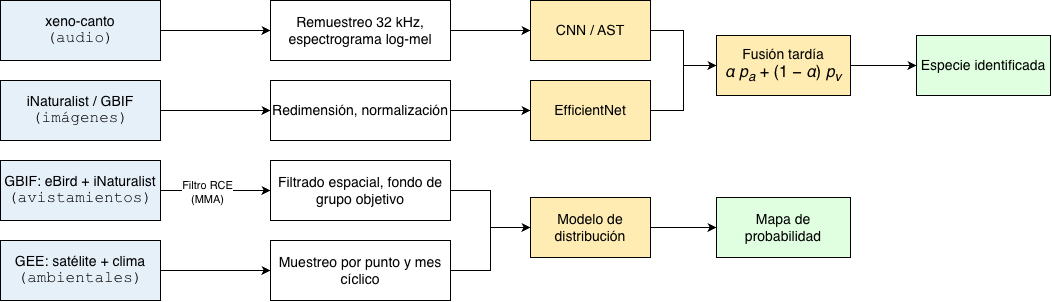
\includegraphics[width=\textwidth]{fig_arquitectura.png}
  \caption{Arquitectura general del sistema: las fuentes de datos (azul) se
  preprocesan (blanco) y alimentan los modelos (amarillo), dos clasificadores
  de audio e imagen cuyas probabilidades se combinan por \textit{late
  fusion}, y un modelo de distribución espaciotemporal comparado con MaxEnt;
  en verde, las salidas. El listado del RCE define las especies objetivo.}
  \label{fig:arquitectura}
\end{figure}

%-----------------------------------------------------------------------
\section{Contribuciones}\label{sec:contribuciones}

Los enfoques previos para la identificación de aves suelen abordar una sola
modalidad. En audio, BirdNET \citep{kahl2021birdnet} es hoy la herramienta
más difundida, pero una evaluación global reciente muestra que su capacidad
predictiva es máxima en Norteamérica, Oceanía y Europa y solo moderada en
Centro y Sudamérica, con \textit{recall} que oscila entre 0,24 y 0,52 según
el continente, lo que refleja diferencias en la cobertura de especies de sus
datos de entrenamiento \citep{funosas2026birdnet}. En imagen, los
clasificadores \textit{fine-grained} se han desarrollado sobre conjuntos como
CUB-200-2011 \citep{wah2011cub} e iNaturalist, dominados por avifaunas del
hemisferio norte. La combinación de audio e imagen para aves ha sido
explorada solo recientemente y con especies norteamericanas
\citep{vanhorn2022ssw60}. En el modelado de distribución,
MaxEnt sigue siendo el método de referencia en ecología y uno de los de
mejor desempeño con datos de solo presencia \citep{elith2011maxent,
valavi2022benchmark}, mientras que los SDM basados en aprendizaje profundo
son un área emergente \citep{deneu2021cnn, cole2023sinr}. No se identificó en
la literatura un sistema integrado que combine identificación multimodal y
modelado de distribución para la avifauna chilena.

Las principales contribuciones de este trabajo son:

\begin{enumerate}[leftmargin=*, itemsep=2pt]
  \item Un \textbf{clasificador multimodal} de 55 especies de aves chilenas
        (53 en ambas modalidades), con \textit{late fusion} de audio e imagen,
        evaluado frente a clasificadores de una sola modalidad (solo audio o
        solo imagen), a clasificadores sobre \textit{frozen embeddings} y a un
        modelo de IA generativa multimodal.
  \item Un \textbf{modelo de distribución espaciotemporal} que integra
        avistamientos, clima, índices de vegetación y elevación, comparado con
        MaxEnt mediante redes neuronales, Random Forest y gradient boosting,
        con partición aleatoria y validación cruzada espacial, incluida una
        evaluación del aporte de los parches de cobertura de suelo y los
        \textit{embeddings} de imágenes satelitales.
  \item Un \textbf{repositorio reproducible} que integra fuentes de datos
        heterogéneas, con un pipeline documentado y reanudable de descarga,
        normalización, partición, entrenamiento y evaluación, y un prototipo
        que integra los modelos, reutilizable para otras especies o regiones.
  \item Una \textbf{caracterización cuantitativa de la escasez de datos} de
        audio, imagen y avistamientos para las especies amenazadas de Chile,
        hallazgo que condiciona el diseño de cualquier sistema de monitoreo
        orientado a la conservación, junto con la evidencia de qué
        estrategias la mitigan en cada modalidad.
\end{enumerate}

\subsection{Contribuciones en términos de precisión}

\begin{enumerate}[leftmargin=*, itemsep=2pt]
  \item El clasificador multimodal supera a los clasificadores de una sola
        modalidad y a un modelo de IA generativa multimodal, y alcanza 0,945
        de \textit{accuracy} sobre 53 especies, por sobre la meta
        del \SI{85}{\percent}, en línea con lo observado en el
        \textit{benchmark} audiovisual SSW60, donde la fusión de modalidades
        supera a cada modalidad por separado. Las ramas de audio (0,858 y
        0,870) e imagen (0,848) cumplen o rozan la meta por sí solas.
  \item El modelo de distribución basado en Random Forest supera a
        MaxEnt en AUC-ROC con partición aleatoria (0,884 frente a 0,863), pero
        no al extrapolar a bloques espaciales no vistos, donde todos los
        modelos empatan. La red neuronal propuesta inicialmente no lo supera
        en ningún protocolo, un resultado negativo que se documenta con
        evidencia y que matiza la expectativa de la literatura sobre SDM
        profundos.
\end{enumerate}

\subsection{Contribuciones en términos de eficacia}

\begin{enumerate}[leftmargin=*, itemsep=2pt]
  \item El sistema automatiza la identificación y el monitoreo, reduce la
        dependencia de inspección experta en terreno y permite procesar
        grandes volúmenes de registros que hoy no pueden revisarse manualmente.
  \item El uso exclusivo de fuentes públicas y de cómputo en la nube (Google
        Earth Engine para el muestreo de las covariables ambientales) elimina
        el costo de adquisición de datos y evita la descarga y el almacenamiento
        local de imágenes satelitales.
  \item Los modelos de distribución permiten priorizar zonas de monitoreo y
        apoyar la planificación territorial para la conservación, en línea con
        las acciones de investigación y monitoreo que promueve la Estrategia
        Nacional de Conservación de Aves.
\end{enumerate}

%-----------------------------------------------------------------------
\section{Estructura del trabajo}\label{sec:estructura}

El resto del documento se organiza como sigue. El \capref{cap:relacionado}
revisa el trabajo relacionado en tres áreas, avanzando desde lo general a lo
específico: identificación bioacústica con aprendizaje profundo,
clasificación de aves por imagen (incluida la fusión multimodal) y modelos
de distribución de especies. El capítulo cierra con una tabla comparativa y la
identificación de la brecha de la literatura. El \capref{cap:teoria} presenta
las bases teóricas: la pregunta de investigación con el objetivo general y
los objetivos específicos, la formalización matemática de los problemas de
clasificación, \textit{late fusion} y distribución, las herramientas, metodologías y
métricas seleccionadas, sus virtudes en el contexto del problema y los
efectos positivos esperados. El \capref{cap:datos} documenta el
levantamiento de datos: la construcción de los corpus de audio, imagen y
avistamientos con sus covariables, los hallazgos derivados de la escasez de
datos en especies amenazadas y las desviaciones respecto del plan. El
\capref{cap:resultados} presenta los resultados de los clasificadores de
audio e imagen, de la fusión multimodal, de los \textit{baselines} de
referencia y del modelo de distribución frente a MaxEnt, junto con el
prototipo integrado y el costo computacional. El \capref{cap:conclusiones}
responde las preguntas de investigación, discute los hallazgos, declara las limitaciones y los aspectos éticos, recoge las lecciones
aprendidas y propone el trabajo futuro.


\chapter{Trabajo relacionado}\label{cap:relacionado}
%=======================================================================
% cap2_trabajo_relacionado.tex
%=======================================================================

Este capítulo revisa el estado del arte en las áreas que sustentan el
proyecto, avanzando desde lo general a lo específico, e identifica la brecha
de la literatura que ofrece la oportunidad de investigación. La revisión se
organiza en tres subáreas: identificación de aves por audio (bioacústica
computacional), identificación por imagen (incluida la fusión multimodal) y
modelos de distribución de especies (SDM). Cada sección describe brevemente la técnica,
revisa los trabajos más influyentes y destaca los aspectos que condicionan el
diseño de esta propuesta. El capítulo cierra con una tabla comparativa
(\tabref{tab:brecha}) y la formulación explícita de la brecha.

%-----------------------------------------------------------------------
\section{Identificación de aves por audio (bioacústica computacional)}
\label{sec:rel-audio}

La bioacústica computacional estudia la detección y clasificación automática
de sonidos animales a partir de grabaciones. Su desarrollo con aprendizaje
profundo ha seguido de cerca al de la clasificación general de audio: la
señal se transforma en una representación tiempo--frecuencia (habitualmente
un espectrograma en escala mel, \secref{sec:teoria-audio}), que se procesa como una imagen mediante redes
convolucionales (CNN, \secref{sec:teoria-cnn}) o, más recientemente, mediante
\textit{transformers} de audio (\secref{sec:teoria-transformers}).

\subsection*{Representaciones de entrada}

El espectrograma mel comprime el eje de frecuencia según una escala
perceptual y expresa la energía en escala logarítmica, lo que concentra la
información relevante para vocalizaciones animales y permite reutilizar
arquitecturas de visión por computador. En este proyecto se adopta el
espectrograma log-mel como representación principal por su compatibilidad
con los modelos preentrenados que se describen a continuación.

\subsection*{Preentrenamiento a gran escala y modelos de referencia}

La disponibilidad de AudioSet, un catálogo de más de dos millones de clips
de audio anotados con 527 clases de sonidos \citep{gemmeke2017audioset},
permitió demostrar que las arquitecturas CNN diseñadas para imágenes
se transfieren de forma efectiva a la clasificación de audio. Sobre esta base se construyeron familias de modelos
de audio preentrenados. Posteriormente, el \textit{Audio Spectrogram
Transformer} (AST) aplicó directamente un \textit{Vision Transformer} a
parches del espectrograma y alcanzó el estado del arte en AudioSet
\citep{gong2021ast}. Su arquitectura se describe en la
\secref{sec:teoria-transformers}. Estos modelos son candidatos naturales para
la identificación bioacústica de especies, dado que sus representaciones
internas codifican patrones espectrotemporales genéricos que pueden
especializarse con relativamente pocos datos.

En el dominio específico de las aves, BirdNET es el modelo más difundido:
una red convolucional profunda con conexiones residuales
(\secref{sec:teoria-cnn}) entrenada sobre espectrogramas de Xeno-canto y
otras colecciones, que en su versión original reconocía 984 especies de
Norteamérica y Europa en grabaciones de campo \citep{kahl2021birdnet}. Las
versiones posteriores superan las \num{6000} especies. Su adopción en
monitoreo acústico pasivo es masiva, pero su desempeño varía fuertemente
entre especies y contextos, por lo que debe validarse localmente antes de
usarse para inferencia ecológica. La
primera evaluación mundial de BirdNET, con \num{4224} grabaciones de 67
sitios en todos los continentes anotadas por expertos locales, confirmó esta
heterogeneidad (\tabref{tab:birdnet}): el desempeño es máximo en los
continentes de donde provienen la mayoría de sus datos de entrenamiento y
cae en Sudamérica \citep{funosas2026birdnet}. Estos resultados justifican
entrenar o adaptar modelos específicos para la avifauna chilena en lugar de
depender de un clasificador global.

\begin{table}[H]
  \centering\small
  \caption{Desempeño de BirdNET por región en la evaluación mundial de
  \citet{funosas2026birdnet}: área bajo la curva precisión--\textit{recall}
  (AUC-PR) por continente; el \textit{recall} varía entre 0,24 y 0,52 según
  el continente.}
  \label{tab:birdnet}
  \begin{tabular}{@{}l l l@{}}
    \toprule
    Región & AUC-PR & Cobertura en los datos de entrenamiento \\
    \midrule
    Norteamérica, Oceanía y Europa & 0,16--0,23 & alta \\
    Centro y Sudamérica & 0,13 & moderada \\
    África y Asia & inferior a 0,13 & baja \\
    \bottomrule
  \end{tabular}
\end{table}

\subsection*{\textit{Embeddings} bioacústicos transferibles}

Una línea reciente muestra que los clasificadores de aves a gran escala
producen \textit{embeddings} que se transfieren mejor a nuevas tareas
bioacústicas que los de modelos de audio general: entrenando clasificadores
lineales sobre las representaciones de BirdNET y de Perch (un modelo de
Google entrenado en Xeno-canto), Ghani \etal\ obtuvieron desempeño superior
a AudioMAE y otros modelos generativos en tareas de aves, anfibios,
mamíferos marinos e insectos, incluso en régimen de pocos ejemplos por clase
\citep{ghani2023embeddings}. El \textit{benchmark} BIRB formaliza esta
evaluación como un problema de recuperación de información con
desplazamiento de distribución entre grabaciones focales y paisajes sonoros
\citep{hamer2023birb}. Esta evidencia importa para las especies con pocas grabaciones, como las
amenazadas de Chile, y justifica considerar el \textit{fine-tuning} de
modelos preentrenados en aves como estrategia complementaria al AST.

\subsection*{Evaluación en condiciones de campo y \textit{benchmarks}}

Los desafíos anuales BirdCLEF son el \textit{benchmark} de referencia: sus ediciones recientes plantean la identificación de especies en
paisajes sonoros continuos de regiones con pocos datos (por ejemplo, África
oriental en 2023), donde los participantes deben lidiar con etiquetas
débiles, solapamiento de vocalizaciones y desplazamiento de dominio entre
las grabaciones focales de Xeno-canto usadas para entrenar y los paisajes
sonoros de prueba \citep{kahl2023birdclef}. Las soluciones ganadoras
combinan CNN preentrenadas, aumentación de datos y ensamblado de modelos.
Xeno-canto, la fuente principal de estos desafíos y de este proyecto, es una
colección de ciencia ciudadana con anotación débil (una especie focal por
grabación, con posibles especies de fondo), duración muy variable y fuerte
desbalance entre especies \citep{vellinga2015xenocanto}.

\subsection*{Desbalance y clases con pocos ejemplos}

El desbalance de clases es inherente a los datos bioacústicos: las especies
comunes acumulan miles de grabaciones y las raras apenas decenas. Entre las
estrategias establecidas está la aumentación en el dominio del
espectrograma, como SpecAugment, que enmascara bandas de tiempo y frecuencia
\citep{park2019specaugment}. Otra es la interpolación de ejemplos mediante
\textit{mixup} \citep{zhang2018mixup}. Una tercera son las funciones de
pérdida que reponderan las clases, como la pérdida focal
\citep{lin2017focal} o la pérdida balanceada por número efectivo de
muestras \citep{cui2019classbalanced}. Estas técnicas conectan directamente con el
hallazgo de escasez de audio en especies amenazadas que se reporta en el
\capref{cap:datos}.

%-----------------------------------------------------------------------
\section{Identificación de aves por imagen y fusión multimodal}
\label{sec:rel-imagen}

\subsection*{Clasificación \textit{fine-grained}}

La identificación de aves por fotografía es el caso paradigmático de la
clasificación visual \textit{fine-grained}: distinguir subcategorías de una
misma clase de objetos (especies dentro del grupo ``aves'') que comparten la
estructura global y difieren en detalles locales, como la forma del pico o
los patrones del plumaje, con alta variabilidad dentro de cada clase por
pose, iluminación y fondo. El conjunto
CUB-200-2011, con \num{11788} imágenes de 200 especies norteamericanas, ha
sido durante más de una década el \textit{benchmark} de referencia.
iNaturalist 2017, con más de \num{850000} imágenes de \num{5089} especies y
datos fuertemente desbalanceados entre clases, acercó el problema a las
condiciones reales de los datos de ciencia ciudadana
\citep{vanhorn2018inaturalist}. En ambos, el \textit{transfer learning}
desde modelos preentrenados en ImageNet es la práctica estándar. Las
arquitecturas residuales establecieron la base. EfficientNet introdujo el
escalado compuesto de profundidad, ancho y resolución, con mejor precisión y
menos parámetros \citep{tan2019efficientnet}. El \textit{Vision Transformer}
mostró que un \textit{transformer} aplicado a parches de imagen supera a las
CNN cuando se preentrena a gran escala \citep{dosovitskiy2021vit}. Las bases
de estas arquitecturas se presentan en el \capref{cap:teoria}.

\subsection*{Estrategias de fusión multimodal}

El aprendizaje multimodal busca representar y combinar información de
distintas modalidades. Según el momento en que ocurre esa combinación,
\citet{baltrusaitis2019multimodal} distinguen tres estrategias:
\textit{early}, \textit{intermediate} y \textit{late fusion}. La primera
concatena las características de entrada y entrena un único clasificador. La
segunda hace interactuar las representaciones latentes de cada rama antes de
decidir. La tercera entrena un clasificador por modalidad y combina sus
probabilidades. Esta última es robusta cuando falta una modalidad en
inferencia, porque basta usar la predicción del clasificador disponible,
permite entrenar cada rama con datos no emparejados y es simple de calibrar.
Su limitación es que no modela interacciones de bajo nivel entre las señales
de entrada. Las tres se formalizan en la \secref{sec:teoria-fusion} y se
comparan empíricamente en el \capref{cap:resultados}.

\subsection*{Fusión audio--imagen en fauna}

La literatura que combina audio e imagen para identificación de animales es
reciente y limitada. El \textit{benchmark} SSW60 (Sapsucker Woods 60), de
Cornell, es el primer conjunto que permite clasificar las mismas 60 especies
de aves en imagen, audio y video. Sus autores muestran que la fusión
audiovisual supera a cada modalidad por separado y que el conocimiento
se transfiere entre modalidades \citep{vanhorn2022ssw60}. Pero sus especies son
norteamericanas y sus datos audiovisuales provienen de video emparejado. No se identificaron trabajos que combinen audio e imagen para
avifauna sudamericana ni que lo hagan a partir de fuentes no emparejadas
(Xeno-canto e iNaturalist), como propone este proyecto.

%-----------------------------------------------------------------------
\section{Modelos de distribución de especies (SDM)}\label{sec:rel-sdm}

Los SDM relacionan registros de ocurrencia de una especie con variables
ambientales para estimar su distribución potencial en el espacio y,
eventualmente, en el tiempo. Constituyen una
herramienta central de la ecología y la planificación de la conservación.

\subsection*{MaxEnt y el problema de solo presencia}

La mayoría de los datos disponibles, incluidos los de ciencia ciudadana,
son de solo presencia: registran dónde se observó una especie, pero no dónde
se buscó sin éxito. MaxEnt aborda este problema con una idea simple: entre todas las formas de
repartir la probabilidad de presencia sobre el territorio, elige la más
``neutra'' posible (la de máxima entropía) que sea compatible con lo
observado, es decir, con que las condiciones ambientales promedio de los
sitios donde se vio la especie coincidan con las del modelo. El resultado es
una probabilidad de presencia que crece de forma exponencial con una
combinación de las covariables, formalmente equivalente a una regresión
logística o de Poisson regularizada \citep{phillips2006maxent}. La
\secref{sec:teoria-sdm} presenta sus ecuaciones. Un \textit{benchmark} reciente con
código reproducible confirma que MaxEnt bien configurado sigue estando entre
los métodos de mejor desempeño para datos de solo presencia, junto con
\textit{boosted regression trees} y ensambles \citep{valavi2022benchmark}, lo
que lo convierte en un \textit{baseline} exigente y no trivial.

\subsection*{Sesgo de muestreo y pseudoausencias}

Como los datos solo dicen dónde se vio a la especie, el modelo necesita
puntos de contraste, las \emph{pseudoausencias} o puntos de fondo, que
representan los lugares donde la especie podría no estar. Si esos puntos se
reparten al azar por el territorio aparece un problema: los registros de
ciencia ciudadana se concentran en zonas accesibles y pobladas, de modo que
el modelo aprende dónde hay observadores en lugar de dónde hay hábitat
adecuado. La solución más usada es elegir los puntos de fondo con el mismo
sesgo que las presencias, por ejemplo, a partir de registros de otras
especies del mismo grupo, lo que mejora sustancialmente las predicciones
\citep{phillips2009bias}. La \figref{fig:fondo-objetivo} del
\capref{cap:teoria} ilustra la diferencia. El número y la ubicación de las
pseudoausencias también influyen en el desempeño, y para eBird existen guías
que recomiendan filtrar por protocolo y esfuerzo y submuestrear espacialmente
\citep{johnston2021ebird}.

\subsection*{SDM con aprendizaje profundo}

Los SDM neuronales reemplazan las funciones de respuesta paramétricas de la
regresión (una curva fija por covariable) por redes que aprenden
interacciones no lineales entre covariables y que pueden compartir
representaciones entre muchas especies, como se formaliza en la
\secref{sec:teoria-sdm}. Botella \etal\ propusieron
el primer enfoque de este tipo a escala continental \citep{botella2018deepsdm}.
Deneu \etal\ demostraron que las CNN que reciben parches de imágenes
ambientales alrededor de cada ocurrencia superan a los modelos puntuales al
capturar la estructura espacial del paisaje \citep{deneu2021cnn}.
Estopinan \etal\ mostraron que incorporar series temporales de Sentinel-2
aporta información estacional que beneficia especialmente a las especies con
pocas ocurrencias \citep{estopinan2022sentinel}. En paralelo, las
representaciones neuronales implícitas espaciales (SINR) codifican
directamente coordenadas y fecha en una red multiespecie entrenada con
registros de iNaturalist, produciendo mapas globales de miles de especies
\citep{cole2023sinr}. Específicamente para aves, SatBird combina imágenes
satelitales y datos de eBird en un conjunto de referencia para predecir tasas
de encuentro de cientos de especies \citep{teng2024satbird}.

\subsection*{Validación espacial}

Los datos de ocurrencia presentan autocorrelación espacial: registros
cercanos comparten ambiente y, si se reparten al azar entre entrenamiento y
prueba, el modelo obtiene estimaciones de desempeño optimistas. Roberts
\etal\ argumentan que la validación cruzada debe respetar la estructura de
los datos mediante bloques espaciales, temporales o jerárquicos
\citep{roberts2017crossvalidation}. El paquete \texttt{blockCV} implementa
la generación de \textit{folds} espacialmente separados y la estimación del rango de
autocorrelación para dimensionar los bloques \citep{valavi2019blockcv}. Este
protocolo se adopta para la comparación entre el SDM neuronal y MaxEnt.

%-----------------------------------------------------------------------
\section{Brecha de la literatura}\label{sec:brecha}

La \tabref{tab:brecha} resume los trabajos más representativos revisados,
según modalidad, región geográfica, número de especies y tarea abordada.

\begin{table}[!htb]
  \centering\footnotesize
  \caption{Comparación del trabajo relacionado y posicionamiento de esta
  propuesta.}
  \label{tab:brecha}
  \begin{tabularx}{\textwidth}{@{}>{\raggedright\arraybackslash\hsize=1.25\hsize}X
    >{\raggedright\arraybackslash\hsize=0.9\hsize}X
    >{\raggedright\arraybackslash\hsize=0.85\hsize}X
    r
    >{\raggedright\arraybackslash}X@{}}
    \toprule
    Trabajo & Modalidad & Región & N.º esp. & Tarea \\
    \midrule
    \citet{kahl2021birdnet} (BirdNET) & Audio & Norteamérica, Europa & 984 & Clasificación \\
    \citet{ghani2023embeddings} & Audio & Global (Xeno-canto) & $>$\num{10000} & Transferencia de \textit{embeddings} \\
    \citet{kahl2023birdclef} (BirdCLEF) & Audio & África oriental & 264 & Detección en paisajes sonoros \\
    \citet{wah2011cub} (CUB-200) & Imagen & Norteamérica & 200 & Clasificación \textit{fine-grained} \\
    \citet{vanhorn2018inaturalist} & Imagen & Global & \num{5089} & Clasificación con datos desbalanceados \\
    \citet{vanhorn2022ssw60} (SSW60) & Audio, imagen, video & Norteamérica & 60 & Clasificación audiovisual \\
    \citet{phillips2006maxent} (MaxEnt) & Ambiental & General & n.a. & Distribución (solo presencia) \\
    \citet{deneu2021cnn} & Ambiental (parches) & Francia & miles (flora) & Distribución (SDM profundo) \\
    \citet{cole2023sinr} (SINR) & Coordenadas + fecha & Global & \num{47375} & Distribución multiespecie \\
    \citet{teng2024satbird} (SatBird) & Satelital + eBird & EE.\,UU./Kenia & 670 & Tasas de encuentro \\
    \midrule
    \textbf{Este trabajo} & \textbf{Audio, imagen, ambiental} & \textbf{Chile continental} & \textbf{55} & \textbf{Clasificación + distribución} \\
    \bottomrule
  \end{tabularx}
\end{table}

A partir de esta revisión se identifican tres brechas concretas. La primera
es geográfica: los clasificadores bioacústicos y visuales de referencia se
entrenan y evalúan sobre avifaunas de Norteamérica y Europa, y la evidencia
global muestra que su desempeño se degrada en Sudamérica. No se identificaron
modelos entrenados para las especies chilenas amenazadas. La segunda es de
modalidad: la fusión de audio e imagen en fauna se ha explorado únicamente
con datos emparejados de especies norteamericanas, sin trabajos que la
apliquen a fuentes de ciencia ciudadana no emparejadas ni a avifaunas del
hemisferio sur. La tercera es de método: los SDM con aprendizaje profundo son
un área emergente que aún no se ha aplicado a la distribución de aves en
Chile, donde la práctica sigue apoyándose en MaxEnt. No existe, por tanto, un
sistema integrado que combine identificación multimodal y modelado de
distribución con aprendizaje profundo para la avifauna chilena. Esa es la
oportunidad que aborda este proyecto.


\chapter{Bases teóricas}\label{cap:teoria}
%=======================================================================
% cap3_bases_teoricas.tex — Bases teóricas
%=======================================================================

Este capítulo plantea las preguntas de investigación y los objetivos sobre
la brecha identificada en el \capref{cap:relacionado} y presenta, desde la
base, los fundamentos de los métodos que usa el sistema: cómo clasifica y
cómo se entrena una red neuronal, qué son una red convolucional y un
\textit{transformer}, cómo se convierte un sonido en una imagen que esas
redes pueden leer, cómo se combinan dos modalidades, cómo se modela la
distribución de una especie a partir de registros de solo presencia y cómo
se evalúa todo lo anterior. Cierra con la metodología de trabajo, las
fuentes de datos y los \textit{baselines}, y con la justificación técnica de
las decisiones tomadas.

%-----------------------------------------------------------------------
\section{Preguntas de investigación, objetivo general y objetivos específicos}
\label{sec:objetivos}

\subsection*{Preguntas de investigación}

\begin{enumerate}[label=\textbf{PI\arabic*.}, leftmargin=*, itemsep=3pt]
  \item ¿Puede un sistema de aprendizaje profundo multimodal identificar
        especies de aves chilenas a partir de audio y/o imagen con mejor
        desempeño que los clasificadores unimodales (solo audio o solo
        imagen) y que un modelo de IA generativa multimodal?
  \item ¿Puede un modelo de distribución de especies basado en aprendizaje
        automático (redes neuronales, Random Forest o gradient boosting), que integra
        avistamientos de ciencia ciudadana, clima e índices de vegetación
        satelitales, superar a MaxEnt bajo un protocolo de validación
        espacial?
  \item ¿Cómo afecta la escasez de datos de las especies amenazadas al
        desempeño de estos modelos? ¿Qué estrategias de aumentación y
        balanceo mitigan ese efecto?
\end{enumerate}

\subsection*{Objetivo general}

Desarrollar y evaluar un sistema de monitoreo de biodiversidad aviar que
integre la identificación multimodal (audio e imagen) y el modelado de
distribución espaciotemporal para especies de aves de Chile continental, con
foco en especies endémicas y amenazadas.

\subsection*{Objetivos específicos}

\begin{enumerate}[label=\textbf{OE\arabic*.}, leftmargin=*, itemsep=3pt]
  \item Construir un conjunto de datos curado y reproducible a partir de
        fuentes heterogéneas (Xeno-canto, iNaturalist/GBIF, registros de
        avistamientos, covariables ambientales satelitales y climáticas vía
        Google Earth Engine y el RCE del MMA), con particiones libres de fuga
        de información.
  \item Entrenar y evaluar clasificadores de audio (CNN/AST) e imagen
        (EfficientNet), e integrarlos mediante \textit{late fusion},
        alcanzando una \textit{accuracy} superior al \SI{85}{\percent} en al
        menos 50 especies.
  \item Entrenar modelos de distribución espaciotemporal basados en
        aprendizaje automático (redes neuronales, Random Forest y gradient boosting) y
        compararlos con un \textit{baseline} MaxEnt, incluida la validación
        cruzada espacial por bloques.
  \item Comparar el clasificador propuesto con un modelo de IA generativa
        multimodal mediante \textit{prompting} (\textit{zero-shot} y
        \textit{few-shot}), para situar su desempeño frente a una herramienta
        de uso general.
  \item Documentar el desempeño (\textit{accuracy}, F1 macro, AUC-ROC, tiempos
        de entrenamiento e inferencia) y las limitaciones, en particular el
        efecto de la escasez de datos en las especies amenazadas.
\end{enumerate}

La meta del \SI{85}{\percent} de \textit{accuracy} del OE2 se fijó en la
propuesta del proyecto como un nivel exigente pero alcanzable para un
problema \textit{fine-grained} de más de cincuenta clases con pocos datos
por especie. Es el nivel a partir del cual un asistente de identificación
acierta en más de cinco de cada seis consultas, lo que lo vuelve útil como
apoyo a un observador. Queda muy por encima de lo que logra el clasificador
global de referencia en Sudamérica (BirdNET, con \textit{recall} entre 0,24
y 0,52 según el continente, \tabref{tab:birdnet}) y es comparable al que
alcanzan los clasificadores regionales entrenados con conjuntos de datos
mucho mayores. Un umbral más bajo no serviría como herramienta de apoyo, y uno
más alto no sería realista con pocas decenas de grabaciones por especie.

%-----------------------------------------------------------------------
\section{Clasificación supervisada con redes neuronales}\label{sec:teoria-redes}

\subsection{El problema de clasificación y la salida softmax}

Clasificar es asignar una entrada $\mathbf{x}$ (una ventana de audio, una
fotografía) a una de $K$ clases disjuntas $\mathcal{C}_1, \dots,
\mathcal{C}_K$, aquí las $K = 55$ especies objetivo. Un clasificador útil no
solo decide: entrega, para cada clase, una probabilidad posterior
$p(\mathcal{C}_k \mid \mathbf{x})$ que expresa cuánta evidencia hay a favor
de esa especie. Separar la estimación de probabilidades de la decisión
final permite rechazar casos dudosos, compensar clases desbalanceadas y
combinar las salidas de varios modelos, que es justamente lo que hará la
fusión multimodal. La regla que
minimiza el número de errores es elegir la clase de mayor probabilidad
posterior \citep[pp.~140--147]{bishop2024deep}:
\begin{equation}
  \hat{y} = \argmax_{k \in \{1,\dots,K\}} \; p(\mathcal{C}_k \mid \mathbf{x}).
  \label{eq:argmax}
\end{equation}

Una red neuronal produce para cada clase un puntaje real $a_k$
(\textit{logit}) y convierte esos puntajes en probabilidades con la función
\textit{softmax}, llamada así porque es una versión suavizada del máximo: si
un puntaje domina a los demás, su probabilidad tiende a uno
\citep[p.~152]{bishop2024deep}:
\begin{equation}
  p(\mathcal{C}_k \mid \mathbf{x}) = y_k = \frac{\exp(a_k)}{\sum_{j=1}^{K} \exp(a_j)},
  \qquad 0 \le y_k \le 1, \quad \sum_{k=1}^{K} y_k = 1.
  \label{eq:softmax}
\end{equation}

\subsection{Verosimilitud y entropía cruzada}

Para entrenar la red hace falta una medida de cuán lejos están sus
probabilidades de las etiquetas verdaderas. Cada etiqueta se codifica como
un vector $\mathbf{t}_n$ con un uno en la clase correcta y ceros en el resto
(codificación 1-de-$K$). La
verosimilitud de las $N$ etiquetas de entrenamiento es el producto de las
probabilidades que la red asigna a las clases correctas, $\prod_n \prod_k
y_{nk}^{t_{nk}}$. Maximizarla equivale a minimizar su logaritmo negativo, la
\emph{entropía cruzada} \citep[p.~162]{bishop2024deep}:
\begin{equation}
  E(\mathbf{w}) = -\sum_{n=1}^{N} \sum_{k=1}^{K} t_{nk} \ln y_k(\mathbf{x}_n, \mathbf{w}),
  \label{eq:ce}
\end{equation}
donde $\mathbf{w}$ reúne todos los parámetros de la red. La entropía cruzada
penaliza con fuerza las predicciones seguras y equivocadas (si $y_k \to 0$
para la clase correcta, $-\ln y_k \to \infty$) y su gradiente respecto de los
logits tiene la forma simple $y_k - t_k$, la diferencia entre la
probabilidad predicha y la etiqueta. Es la
pérdida con que se entrenan todos los clasificadores de esta tesis.

Cuando las clases tienen tamaños muy distintos, la red tiende a favorecer a
las mayoritarias. Una corrección habitual es ponderar la pérdida de cada
clase por un peso $\omega_k$ que decrece con su número de ejemplos $n_k$. La
pérdida balanceada por número efectivo de muestras usa $\omega_k \propto
(1-\beta)/(1-\beta^{n_k})$ \citep{cui2019classbalanced}. En el límite $\beta
\to 1$ el peso tiende a $1/n_k$, el inverso de la frecuencia, que es la
variante implementada aquí (normalizada para que los pesos promedien uno):
\begin{equation}
  E_{\mathrm{pond}}(\mathbf{w}) = -\sum_{n=1}^{N} \sum_{k=1}^{K} \omega_k\, t_{nk} \ln y_{nk},
  \qquad \omega_k = \frac{1/n_k}{\frac{1}{K}\sum_{j=1}^{K} 1/n_j}.
  \label{eq:ce-pond}
\end{equation}

\subsection{Redes neuronales y su entrenamiento}

Una red neuronal es una composición de transformaciones lineales y
funciones no lineales. En la forma más simple, el perceptrón multicapa, cada
capa $l$ calcula $\mathbf{z}^{(l)} = h\big(\mathbf{W}^{(l)} \mathbf{z}^{(l-1)}\big)$ a
partir de la salida de la capa anterior, con $\mathbf{z}^{(0)} = \mathbf{x}$ y
$\mathbf{W}^{(l)}$ una matriz de pesos aprendibles
\citep[pp.~181--187]{bishop2024deep}. La no linealidad $h$ es imprescindible: sin
ella toda la red colapsaría en un modelo lineal. La más usada es la unidad
lineal rectificada, $\mathrm{ReLU}(a) = \max(0, a)$, barata y libre del
problema de los gradientes que se desvanecen con la sigmoide. Con
suficientes unidades, una red de
dos capas puede aproximar cualquier función continua, pero el teorema solo
garantiza la existencia. En la práctica la profundidad permite representar
la misma función con muchos menos parámetros y aprender representaciones
jerárquicas, de rasgos simples a conceptos.

El entrenamiento minimiza la pérdida por \emph{descenso de gradiente}: en
cada paso los parámetros se mueven en la dirección contraria al gradiente,
$\mathbf{w}^{(\tau)} = \mathbf{w}^{(\tau-1)} - \eta \nabla E(\mathbf{w}^{(\tau-1)})$,
con una tasa de aprendizaje $\eta$. Como el
gradiente sobre todo el conjunto es costoso, se estima sobre minilotes de
$n_b$ ejemplos (descenso de gradiente estocástico). Una pasada completa por
los datos es una \emph{época}. El gradiente de cada parámetro se obtiene por
retropropagación. El optimizador Adam mantiene promedios móviles del
gradiente ($s_i$) y de su cuadrado ($r_i$) para adaptar el tamaño del paso a
cada parámetro \citep[pp.~222--224]{bishop2024deep}:
\begin{equation}
  w_i^{(\tau)} = w_i^{(\tau-1)} - \eta\, \frac{\hat{s}_i}{\sqrt{\hat{r}_i} + \delta},
  \label{eq:adam}
\end{equation}
con $\hat{s}_i$ y $\hat{r}_i$ corregidos por el sesgo de su inicialización en
cero y $\delta$ una constante pequeña de estabilidad. La variante AdamW,
usada en esta tesis, aplica el decaimiento de pesos de forma desacoplada del
gradiente \citep{loshchilov2019adamw}. La tasa de aprendizaje se reduce a
lo largo del entrenamiento (programación de coseno), porque conviene
empezar con pasos grandes y terminar con pasos finos.

%-----------------------------------------------------------------------
\section{Sobreajuste, regularización y aumentación de datos}\label{sec:teoria-regularizacion}

Una red con millones de parámetros puede memorizar el conjunto de
entrenamiento, incluido su ruido, y fallar con datos nuevos: es el
\emph{sobreajuste}. Se detecta comparando el error de entrenamiento con el de
un conjunto de validación: el primero baja siempre, mientras que el segundo
baja y luego sube cuando la red empieza a memorizar \citep[pp.~266--267]{bishop2024deep}.
La \emph{regularización} agrupa las técnicas que inducen a la red a preferir
soluciones más simples o más invariantes. La experiencia práctica se resume
en una regla: casi siempre generaliza mejor una red grande con
regularización que una red pequeña sin ella \citep[p.~254]{bishop2024deep}.
Las técnicas usadas en esta tesis son las siguientes.

\begin{itemize}[leftmargin=*, itemsep=2pt]
  \item \textbf{Decaimiento de pesos.} Se agrega a la pérdida un término
        $\frac{\lambda_{\mathrm{wd}}}{2}\mathbf{w}^{\mathrm{T}}\mathbf{w}$ que penaliza los pesos
        grandes. Su gradiente $\lambda_{\mathrm{wd}} \mathbf{w}$ empuja cada peso hacia cero
        salvo que los datos lo sostengan \citep[p.~260]{bishop2024deep}.
  \item \textbf{Parada temprana.} Se conserva el modelo de la época con mejor
        desempeño en validación, lo que limita cuánto puede ajustarse la red.
  \item \textbf{\textit{Dropout}.} Durante el entrenamiento se desactivan al
        azar unidades de la red. La red resultante es un promedio aproximado
        de muchas subredes y ninguna unidad puede depender de otra
        específica \citep[pp.~279--281]{bishop2024deep}.
  \item \textbf{Profundidad estocástica.} En redes con bloques residuales
        (\secref{sec:teoria-cnn}) se omiten bloques completos al azar, con
        probabilidad creciente hacia la salida. Acorta la red durante el
        entrenamiento y regulariza como el \textit{dropout}, pero a nivel de
        bloque \citep{huang2016stochasticdepth}.
  \item \textbf{Suavizado de etiquetas.} En vez de exigir probabilidad uno
        para la clase correcta, la etiqueta se reparte: $t_k = 1-\epsilon+\epsilon/K$
        para la clase correcta y $\epsilon/K$ para las demás (la variante
        que implementa PyTorch), con $\epsilon = 0{,}1$. Evita que la red se vuelva demasiado segura y
        mejora la calibración de sus probabilidades
        \citep{szegedy2016labelsmoothing}.
  \item \textbf{Aumentación de datos.} Se amplía el conjunto de entrenamiento
        con copias transformadas de cada ejemplo que conservan la etiqueta:
        recortes, volteos y cambios de color en imágenes, o ruido y cambios
        de ganancia en audio. Cada vez que el ejemplo se presenta se aplica
        una transformación distinta \citep[pp.~257--258]{bishop2024deep}.
        Es la forma más efectiva de enseñar invariancias cuando hay pocos
        datos.
  \item \textbf{\textit{Mixup}.} Se entrena con mezclas convexas de pares de
        ejemplos y de sus etiquetas \citep{zhang2018mixup}:
        \begin{equation}
          \tilde{\mathbf{x}} = \lambda \mathbf{x}_i + (1-\lambda)\mathbf{x}_j, \qquad
          \tilde{\mathbf{t}} = \lambda \mathbf{t}_i + (1-\lambda)\mathbf{t}_j, \qquad
          \lambda \sim \mathrm{Beta}(a, a),
          \label{eq:mixup}
        \end{equation}
        lo que obliga a la red a comportarse de forma suave entre ejemplos y
        reduce la memorización. Aquí $a = 0{,}2$.
  \item \textbf{SpecAugment.} Aumentación específica de espectrogramas: se
        enmascaran franjas aleatorias de frecuencia y de tiempo, de modo que
        la red no pueda apoyarse en una sola banda o en un solo instante del
        canto \citep{park2019specaugment}. La
        \figref{fig:representacion-audio} muestra un ejemplo de ambas
        aumentaciones de audio.
\end{itemize}

%-----------------------------------------------------------------------
\section{Redes convolucionales y EfficientNet}\label{sec:teoria-cnn}

\subsection{La operación de convolución}

Una fotografía (o un espectrograma) es una grilla de valores con fuerte
estructura local: dos píxeles vecinos suelen parecerse y un rasgo (un borde,
una mancha, un trino) ocupa una región pequeña y puede aparecer en cualquier
posición. Una red densa ignora esa estructura y necesitaría miles de
millones de pesos para una imagen de alta resolución. La red convolucional
(CNN) incorpora en su diseño la localidad, la jerarquía, la equivariancia y
la invariancia a traslaciones, y por eso necesita muchos menos datos
\citep[pp.~289--290]{bishop2024deep}. Su operación básica, la
\emph{convolución}, desliza un pequeño filtro o \textit{kernel} $\mathbf{U}$
de $s \times s$ pesos sobre toda la entrada $\mathbf{I}$ y calcula en cada
posición el producto punto entre el filtro y el parche que cubre
\citep[p.~292]{bishop2024deep}:
\begin{equation}
  C(p, q) = \sum_{l=1}^{s} \sum_{m=1}^{s} I(p+l,\, q+m)\, u_{lm} + b,
  \label{eq:conv}
\end{equation}
donde $C$ es el \emph{mapa de características}, $u_{lm}$ los pesos del
filtro y $b$ un sesgo. Cada filtro
actúa como un detector que se ``enciende'' (tras la ReLU) cuando el parche se
parece a su patrón. Como el mismo filtro recorre toda la imagen, un rasgo se
detecta esté donde esté, con muy pocos parámetros. Una capa aplica
$C_{\mathrm{out}}$ filtros distintos sobre los $C_{\mathrm{in}}$ canales de
entrada, con $(s^2 C_{\mathrm{in}} + 1)\,C_{\mathrm{out}}$ parámetros en
total. El \emph{pooling} resume bloques
vecinos con el máximo o el promedio: conserva si un rasgo está presente y
con qué fuerza, descarta parte de su posición exacta y reduce la
resolución, de modo que las capas siguientes ``ven'' regiones cada vez
mayores \citep[pp.~296--298]{bishop2024deep}. Apilando capas de convolución
y \textit{pooling}, los rasgos simples de las primeras capas (bordes, tonos
sostenidos) se combinan en patrones complejos (un pico, una sílaba del
canto) y, al final, un \textit{pooling} global y una capa densa con softmax
producen las $K$ probabilidades (\figref{fig:cnn}).

\begin{figure}[!htb]
  \centering
  \IfFileExists{figuras/tikz_cnn.tex}{\fitwidth{% Figura: red neuronal convolucional (tres paneles apilados).
% (a) operación de convolución, (b) arquitectura típica, (c) bloque residual.
% Unidades: 1 = 1 mm. Ancho total ~150 mm x alto ~125 mm (cabe en \textwidth = 160 mm).
\begin{tikzpicture}[x=1mm, y=1mm, font=\footnotesize,
  bloque/.style={draw, rounded corners, align=center, minimum height=8mm,
                 minimum width=20mm, font=\footnotesize, inner sep=1.5pt},
  dato/.style={bloque, fill=pucazul!15},
  capa/.style={bloque, fill=miaamarillo!30},
  proc/.style={bloque, fill=black!5},
  salida/.style={bloque, fill=green!12},
  flecha/.style={-{Latex[length=2mm]}, thick},
  flechita/.style={-{Latex[length=1.5mm]}, thin, pucgris},
  panel/.style={anchor=north west, font=\footnotesize\bfseries, inner sep=0pt},
  etq/.style={font=\footnotesize, align=center, inner sep=1pt},
  mini/.style={font=\scriptsize, align=center, inner sep=1pt}]

  % Pila de mapas de características: \pila{x}{lado}{n}{desplazamiento}{relleno}{nombre}
  \def\pila#1#2#3#4#5#6{%
    \foreach \k in {#3,...,1}{%
      \pgfmathsetmacro{\kk}{\k-1}%
      \draw[draw=pucgris, thin, rounded corners=0.4mm, fill=#5]
        ({#1+\kk*#4},{-#2/2+\kk*#4}) rectangle ++(#2,#2);}%
    \coordinate (#6w) at (#1,0);
    \coordinate (#6e) at ({#1+#2+min(#3-1,floor(#2/2/#4))*#4},0);}

  % ================= (a) Operación de convolución =================
  \begin{scope}[shift={(4,0)}]
    \node[panel] at (-4,36) {(a) Operación de convolución};
    % Entrada 6x6
    \begin{scope}[shift={(4,2)}]
      \foreach \i in {0,...,5} \foreach \j in {0,...,5}
        \fill[pucazul!15] (4*\i,4*\j) rectangle ++(4,4);
      % celdas "de señal" (coordenadas en mm; celda = 4 mm)
      \foreach \c in {(0,4),(4,4),(8,0),(16,8),(20,12),(20,16),(0,20),(12,20)}
        \fill[pucazul!40] \c rectangle ++(4,4);
      % ventana desplazada (punteada) debajo del relleno amarillo
      \draw[pucgris, thick, dashed] (8,8) rectangle (20,20);
      \fill[miaamarillo!50] (4,8) rectangle (16,20);
      \draw[pucgris!50, very thin] (0,0) grid[step=4] (24,24);
      \draw[pucgris, thick] (4,8) rectangle (16,20);
      \draw[flechita] (9,25.5) -- (15,25.5);
      \node[mini, anchor=south] at (12,26.3) {se desliza};
      \node[etq, anchor=north] at (12,-1) {Entrada\\(espectrograma o imagen)};
    \end{scope}
    % Filtro 3x3
    \draw[flecha] (28,14) -- (36,14) node[midway, above=0.3mm, mini] {$\ast$};
    \begin{scope}[shift={(36,8.75)}]
      \foreach \i in {0,1,2} \foreach \j in {0,1,2}
        \fill[miaamarillo!50] (3.5*\i,3.5*\j) rectangle ++(3.5,3.5);
      \draw[pucgris, very thin] (0,0) grid[step=3.5] (10.5,10.5);
      \draw[pucgris, thick] (0,0) rectangle (10.5,10.5);
      \node[etq, anchor=south] at (5.25,11.5) {Filtro $3{\times}3$};
      \node[mini, anchor=north] at (5.25,-1) {pesos $u_{l,m}$, sesgo $b$};
    \end{scope}
    % Mapa de características 4x4
    \draw[flecha] (46.5,14) -- (54.5,14);
    \begin{scope}[shift={(54.5,6)}]
      \foreach \i in {0,...,3} \foreach \j in {0,...,3}
        \fill[pucazul!15] (4*\i,4*\j) rectangle ++(4,4);
      \foreach \c in {(0,0),(12,4),(8,12)}
        \fill[pucazul!40] \c rectangle ++(4,4);
      \fill[miaamarillo!50] (4,8) rectangle (8,12);
      \draw[pucgris!50, very thin] (0,0) grid[step=4] (16,16);
      \draw[pucgris, thick] (4,8) rectangle (8,12);
      \node[etq, anchor=north] at (8,-1) {Mapa de\\características};
    \end{scope}
    % Fórmula
    \node[anchor=west, align=left, inner sep=0pt] at (75,14)
      {$\displaystyle C_{p,q} = \sum_{l,m} I_{p+l,\,q+m}\, u_{l,m} + b$\\[2mm]
       seguida de ReLU: $\max(0,\,C_{p,q})$};
  \end{scope}

  % ================= (b) Arquitectura típica =================
  \begin{scope}[shift={(0,-32)}]
    \node[panel] at (0,20) {(b) Arquitectura típica de una CNN para clasificación};
    % Entrada
    \draw[draw=pucgris, thin, rounded corners=0.4mm, fill=pucazul!15] (0,-6) rectangle (12,6);
    \node[mini, anchor=south] at (6,9.2) {$H\times W$};
    \node[etq, anchor=north] at (6,-6.8) {Entrada};
    % Bloques convolución + pooling (x3)
    \pila{18.5}{11}{3}{1.2}{miaamarillo!30}{c1}
    \pila{38.4}{8}{3}{1.2}{black!5}{p1}
    \pila{55.3}{8}{4}{1.1}{miaamarillo!30}{c2}
    \pila{73.1}{6}{4}{1.1}{black!5}{p2}
    \pila{88.9}{6}{5}{1.0}{miaamarillo!30}{c3}
    \pila{105.4}{4.5}{5}{1.0}{black!5}{p3}
    \node[etq, anchor=north] at (25.2,-6.8) {Convolución\\+ ReLU};
    \node[etq, anchor=north] at (60.95,-6.8) {Convolución\\+ ReLU};
    \node[etq, anchor=north] at (93.9,-6.8) {Convolución\\+ ReLU};
    \node[mini, anchor=south] at (25.2,9.2) {$C_1$ canales};
    \node[mini, anchor=south] at (60.95,9.2) {$C_2 > C_1$};
    \node[mini, anchor=south] at (93.9,9.2) {$C_3 > C_2$};
    \node[etq, anchor=south] at (43.6,9.2) {Pooling};
    \node[etq, anchor=south] at (77.75,9.2) {Pooling};
    \node[etq, anchor=south] at (109.65,9.2) {Pooling};
    % Pooling global -> vector
    \draw[draw=pucgris, thin, fill=black!5] (120.4,-6) rectangle (123.4,6);
    \foreach \y in {-4.5,-3,...,4.5} \draw[pucgris!50, very thin] (120.4,\y) -- (123.4,\y);
    \node[etq, anchor=north] at (121.9,-6.8) {Pooling\\global};
    % Capa densa
    \draw[draw=pucgris, thin, fill=miaamarillo!30] (129.9,-4) rectangle (132.9,4);
    \foreach \y in {-2.4,-0.8,0.8,2.4} \draw[pucgris!50, very thin] (129.9,\y) -- (132.9,\y);
    \node[etq, anchor=south] at (131.4,9.2) {Capa densa\\($K$ logits)};
    % Softmax
    \draw[draw=pucgris, thin, fill=green!12] (139.4,-4) rectangle (142.4,4);
    \fill[green!45] (139.4,0.8) rectangle (142.4,2.4);
    \foreach \y in {-2.4,-0.8,0.8,2.4} \draw[pucgris!50, very thin] (139.4,\y) -- (142.4,\y);
    \node[etq, anchor=north] at (140.9,-6.8) {Softmax\\($K$ especies)};
    % Flechas
    \draw[flecha] (12,0) -- (c1w);
    \draw[flecha] (c1e) -- (p1w);
    \draw[flecha] (p1e) -- (c2w);
    \draw[flecha] (c2e) -- (p2w);
    \draw[flecha] (p2e) -- (c3w);
    \draw[flecha] (c3e) -- (p3w);
    \draw[flecha] (p3e) -- (120.4,0);
    \draw[flecha] (123.4,0) -- (129.9,0);
    \draw[flecha] (132.9,0) -- (139.4,0);
    % Tendencia
    \draw[flechita] (18.5,-17.5) -- (113.9,-17.5);
    \node[mini, anchor=north] at (66.2,-18.2)
      {mapas de características cada vez más pequeños y con más canales};
  \end{scope}

  % ================= (c) Bloque residual =================
  \begin{scope}[shift={(0,-76.5)}]
    \node[panel] at (0,19.5) {(c) Bloque con conexión residual};
    \node[dato, minimum width=8mm] (rx) at (4,0) {$x$};
    \node[capa, right=6.5mm of rx, minimum width=22mm] (f1) {Convolución\\+ ReLU};
    \node[capa, right=6.5mm of f1, minimum width=22mm] (f2) {Convolución};
    \node[draw, circle, fill=black!5, minimum size=5mm, inner sep=0pt,
          right=6.5mm of f2] (sum) {$+$};
    \node[salida, right=6.5mm of sum, minimum width=22mm] (ry) {$y = F(x) + x$};
    \draw[flecha] (rx) -- (f1);
    \draw[flecha] (f1) -- (f2);
    \draw[flecha] (f2) -- (sum);
    \draw[flecha] (sum) -- (ry);
    \draw[flecha] (rx.north) -- ++(0,6) -| (sum.north)
      node[pos=0.25, above, etq] {Conexión residual (atajo de identidad, $x$)};
    \draw[decorate, decoration={brace, mirror, amplitude=1.5mm}]
      ([yshift=-1.5mm]f1.south west) -- ([yshift=-1.5mm]f2.south east)
      node[midway, below=2mm, etq] {$F(x)$: residuo aprendido por las capas};
  \end{scope}
\end{tikzpicture}
}}{\fbox{figura pendiente}}
  \caption{Elementos de una red convolucional: (a) un filtro de $3\times3$
  recorre la entrada y produce el mapa de características
  (Ecuación~\ref{eq:conv}); (b) arquitectura típica de clasificación, con
  bloques de convolución y \textit{pooling} seguidos de \textit{pooling}
  global, capa densa y softmax; (c) bloque residual
  (Ecuación~\ref{eq:residual}). Elaboración propia a partir de
  \citet{bishop2024deep} y \citet{he2016resnet}.}
  \label{fig:cnn}
\end{figure}

\subsection{Conexiones residuales}

Al apilar decenas de capas el entrenamiento se vuelve inestable: el
gradiente que llega a las primeras capas se degrada y la red profunda rinde
peor que una más corta. La solución de las redes residuales (ResNet) es
sumar la entrada de cada bloque a su salida \citep{he2016resnet}:
\begin{equation}
  \mathbf{z}_l = \mathbf{F}_l(\mathbf{z}_{l-1}) + \mathbf{z}_{l-1},
  \label{eq:residual}
\end{equation}
de modo que el bloque aprende solo el \emph{residuo} respecto de la
identidad, que puede reproducirse con pesos pequeños. Esto suaviza la
superficie de error y permite entrenar redes de cientos de capas. BirdNET,
EfficientNet y los
\textit{transformers} usan conexiones residuales.

\subsection{EfficientNet}

EfficientNet \citep{tan2019efficientnet} es la familia de CNN que usa esta
tesis en ambas modalidades. Su bloque básico, MBConv, es un bloque residual ``invertido'': una
convolución $1 \times 1$ expande los canales (por seis), una convolución
\textit{depthwise} de $3 \times 3$ o $5 \times 5$ filtra cada canal por
separado (mucho más barata que una convolución completa), un módulo
\textit{squeeze-and-excitation} reescala los canales según su importancia
global y una convolución $1 \times 1$ proyecta de vuelta al número de
canales original, donde se suma el atajo residual. EfficientNet-B0 encadena
un \textit{stem} convolucional, siete etapas con 16 bloques MBConv en
total, una convolución $1 \times 1$ a 1\,280 canales, \textit{pooling}
global y la capa de clasificación; \citet{tan2019efficientnet}
muestran el esquema completo. Con 4,1 millones de
parámetros es la CNN de audio de esta tesis. La contribución metodológica de
EfficientNet es el \emph{escalado compuesto}: en lugar de agrandar la red
solo en profundidad, ancho o resolución, los tres se escalan juntos con un
único exponente $\phi$,
\begin{equation}
  d = \alpha^{\phi}, \qquad w = \beta^{\phi}, \qquad r = \gamma^{\phi},
  \qquad \alpha\,\beta^{2}\gamma^{2} \approx 2,
  \label{eq:compound}
\end{equation}
con $\alpha, \beta, \gamma \ge 1$ fijados por una búsqueda sobre B0, de modo que
cada incremento de $\phi$ duplica aproximadamente el costo de cómputo. B3,
el tercer paso de la familia (profundidad $\times 1{,}4$ y ancho
$\times 1{,}2$ respecto de B0, resolución nativa de \SI{300}{px}), tiene
10,8 millones de parámetros y es el clasificador de imagen; aquí se usa con
una entrada de \SI{384}{px}.


%-----------------------------------------------------------------------
\section{\textit{Transformers}: atención, ViT y AST}\label{sec:teoria-transformers}

\subsection{Atención}

Un \textit{transformer} procesa un conjunto de $N$ vectores o
\emph{tokens} (palabras de una frase, parches de una imagen, trozos de un
espectrograma) y produce otro conjunto de $N$ vectores con una
representación más rica \citep[p.~357]{bishop2024deep}. Su operación
central, la \emph{atención}, construye cada salida como una mezcla de todas
las entradas con pesos que dependen de los propios datos: para interpretar
un token, la red ``mira'' con más peso a los tokens relevantes, estén donde
estén. Cada token genera tres vectores mediante matrices aprendibles: una
\emph{consulta} $\mathbf{q}$, una \emph{clave} $\mathbf{k}$ y un \emph{valor}
$\mathbf{v}$. La similitud consulta--clave se mide con el producto punto, se
normaliza con un softmax y pondera los valores
\citep{vaswani2017attention}:
\begin{equation}
  \text{Atención}(\mathbf{Q}, \mathbf{K}, \mathbf{V}) =
  \mathrm{softmax}\!\left(\frac{\mathbf{Q}\mathbf{K}^{\mathrm{T}}}{\sqrt{D_k}}\right)\mathbf{V},
  \qquad \mathbf{Q} = \mathbf{X}\mathbf{W}^{(q)},\;
  \mathbf{K} = \mathbf{X}\mathbf{W}^{(k)},\;
  \mathbf{V} = \mathbf{X}\mathbf{W}^{(v)},
  \label{eq:attention}
\end{equation}
donde $\mathbf{X}$ apila los $N$ tokens como filas y $D_k$ es la dimensión de
las claves. Dividir por $\sqrt{D_k}$ evita que el softmax se sature. Una
sola cabeza tiende a promediar patrones
distintos, así que se usan $n_h$ cabezas en paralelo con parámetros propios,
cuyas salidas se concatenan y proyectan: es el análogo de usar varios filtros
en una capa convolucional. Un bloque
codificador alterna la atención multicabeza, que mezcla información
\emph{entre} tokens, con un perceptrón multicapa compartido, que transforma
cada token por separado, ambos con conexión residual y normalización de
capa. Como las matrices se comparten entre tokens, el modelo no sabe en qué
posición está cada uno, y por eso se suma a cada token un vector de posición
aprendido \citep[pp.~366--374]{bishop2024deep}.

\subsection{Vision Transformer y Audio Spectrogram Transformer}

Aplicar atención a cada píxel es inviable, porque el costo crece con el
cuadrado del número de tokens. El \textit{Vision Transformer} (ViT) divide
la imagen en parches de $P \times P$ píxeles ($P = 16$), aplana cada parche y
lo proyecta linealmente a un vector de dimensión $D$, obteniendo $N =
H_{\mathrm{img}} W_{\mathrm{img}}/P^2$ tokens para una imagen de
$H_{\mathrm{img}} \times W_{\mathrm{img}}$ píxeles \citep{dosovitskiy2021vit}. Se antepone un token especial de
clase cuya salida, tras los bloques codificadores, alimenta la capa de
clasificación. El \textit{Audio
Spectrogram Transformer} (AST) aplica exactamente el mismo diseño al
espectrograma log-mel tratado como imagen \citep{gong2021ast}: parches de
$16 \times 16$ con paso de 10 (solapados), proyección a $D = 768$, embedding
posicional, token de clase, 12 bloques codificadores con 12 cabezas y una
capa densa de $K$ salidas (\figref{fig:ast}). El modelo de esta tesis tiene
86,2 millones de parámetros, veinte veces más que la CNN. A diferencia de la
CNN, que capta bien relaciones locales pero tiene dificultades con
dependencias de largo alcance en el espectrograma, la atención conecta
cualquier par de parches desde la primera capa
\citep[p.~400]{bishop2024deep}. El precio es que, al tener menos sesgos
inductivos, necesita más datos o un buen preentrenamiento.

\begin{figure}[!htb]
  \centering
  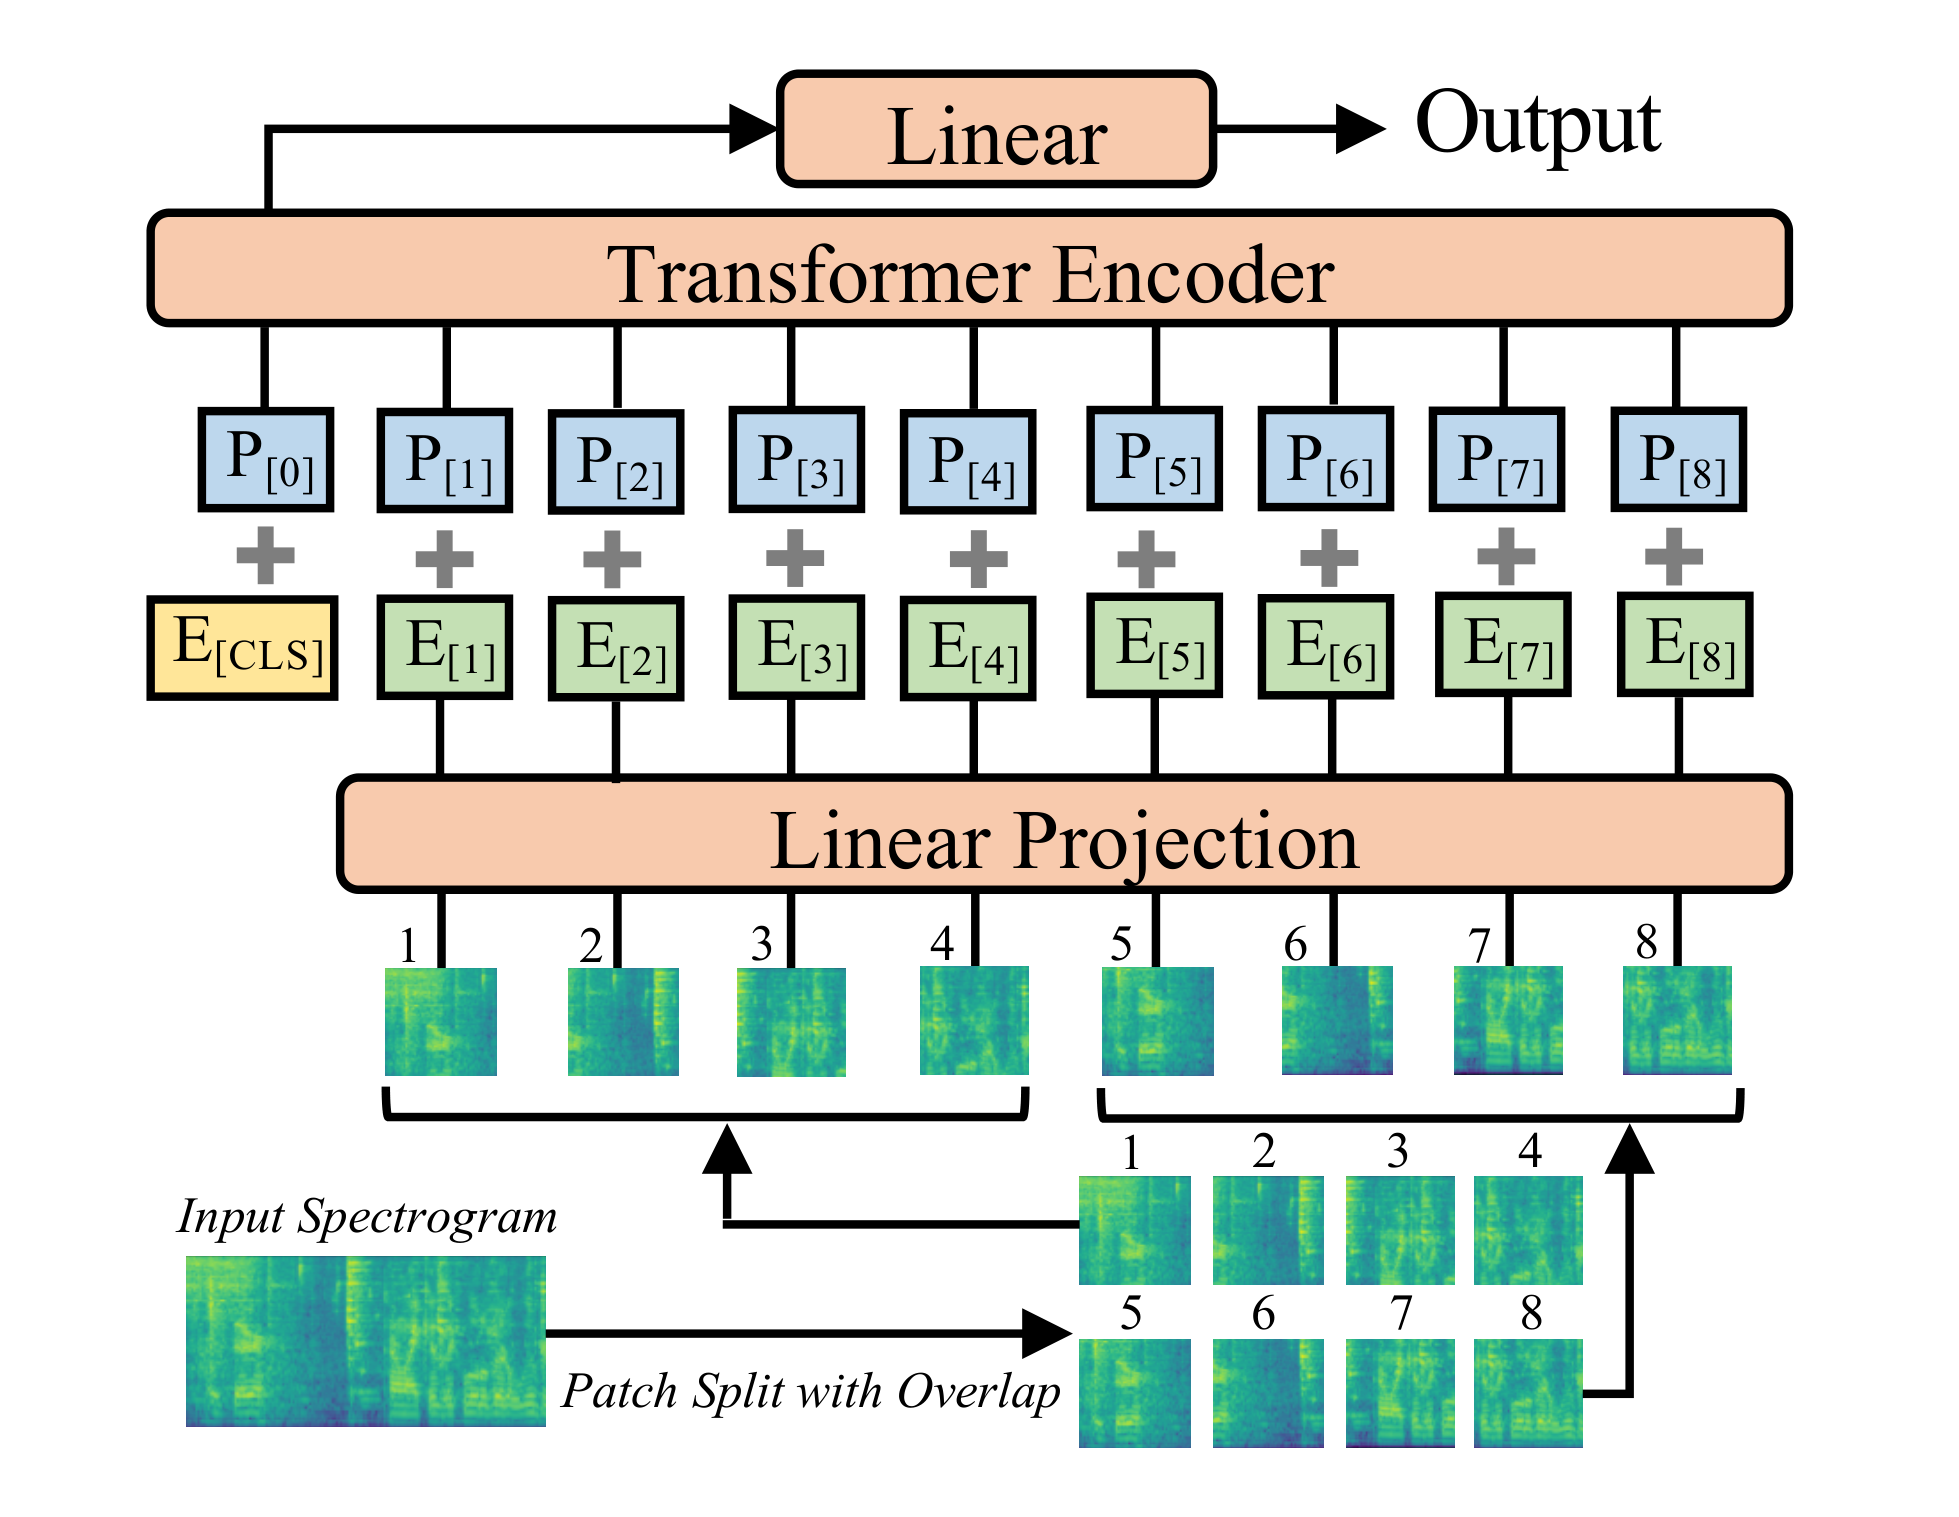
\includegraphics[width=0.62\textwidth]{fig_ast_gong2021.png}
  \caption{Arquitectura del \textit{Audio Spectrogram Transformer}: el
  espectrograma se divide en parches de $16\times16$ con solapamiento, cada
  parche se proyecta linealmente y, con su embedding posicional y el token de
  clase, atraviesa el codificador \textit{Transformer}; la salida del token
  de clase alimenta la capa de clasificación. Tomada de \citet{gong2021ast}.}
  \label{fig:ast}
\end{figure}

%-----------------------------------------------------------------------
\section{\textit{Transfer learning} y \textit{frozen embeddings}}\label{sec:teoria-transfer}

Una red entrenada con millones de imágenes naturales aprende en sus primeras
capas rasgos genéricos (bordes, texturas) y en las últimas rasgos propios de
su tarea. Para un problema nuevo con pocos datos, el \textit{transfer
learning} reutiliza esa red preentrenada: se reemplaza la capa de
clasificación por una de $K$ salidas y se reentrena toda la red con una tasa
de aprendizaje pequeña (\textit{fine-tuning}), o bien se congela el cuerpo
de la red y se entrena solo la nueva capa
\citep[pp.~189--190]{bishop2024deep}. El segundo caso equivale a usar la red
como extractor de características fijas, sus \textit{frozen embeddings}, y
ajustar un clasificador lineal encima. Es la referencia de bajo costo que
\citet{ghani2023embeddings} proponen para bioacústica y uno de los
\textit{baselines} de esta tesis. Aquí se ajustan por completo una
EfficientNet-B0 de ImageNet para audio, una EfficientNet-B3 de ImageNet para
imagen y un AST preentrenado en AudioSet, y ese ajuste se compara con los
\textit{frozen embeddings} de los mismos modelos; como comparación en imagen
se ajusta además un ViT-S/16 preentrenado en ImageNet-21k.

%-----------------------------------------------------------------------
\section{Del audio al espectrograma log-mel}\label{sec:teoria-audio}

\subsection{Señal, muestreo y transformada de Fourier}

Un sonido es una variación de la presión del aire en el tiempo. Al grabarlo,
el computador lo muestrea: lee el valor de la señal $F_s$ veces por segundo
(la \emph{frecuencia de muestreo}; la CNN de esta tesis trabaja a
\SI{32}{\kilo\hertz}), lo
que da una secuencia de números $x(n)$. El teorema de muestreo garantiza que
no se pierde información si la señal no contiene frecuencias superiores a
$F_s/2$, la frecuencia de Nyquist \citep[pp.~50, 61]{muller2021fmp}. Con
\SI{32}{\kilo\hertz} se cubren hasta \SI{16}{\kilo\hertz}, suficiente para
las vocalizaciones de aves, que rara vez superan los
\SIrange{10}{12}{\kilo\hertz}.

La forma de onda muestra cuándo suena algo pero oculta qué frecuencias
contiene. La transformada de Fourier hace lo contrario
\citep[pp.~39--41]{muller2021fmp}. Compara la señal con sinusoides de cada
frecuencia: el coeficiente es grande cuando la señal ``sube y baja'' al
ritmo de esa sinusoide. Para una secuencia de $L$ muestras, la transformada
discreta de Fourier (DFT) es \citep[p.~52]{muller2021fmp}
\begin{equation}
  X(k) = \sum_{n=0}^{L-1} x(n)\, e^{-2\pi i k n / L}, \qquad k = 0, \dots, L-1,
  \label{eq:dft}
\end{equation}
donde el índice $k$ corresponde a la frecuencia física $k F_s / L$ hercios.
Para no perder el ``cuándo'', la transformada de Fourier de tiempo corto
(STFT) aplica la DFT a tramos cortos de la señal: se multiplica la señal por
una ventana $w$ de $L$ muestras (en la CNN, $L = 1024$, \SI{32}{\milli\second}),
se calcula la DFT y se desplaza la ventana en pasos de $H$ muestras ($H
= 320$, \SI{10}{\milli\second}) \citep[pp.~53--55]{muller2021fmp}:
\begin{equation}
  \mathcal{X}(m, k) = \sum_{n=0}^{L-1} x(n + mH)\, w(n)\, e^{-2\pi i k n / L}.
  \label{eq:stft}
\end{equation}
El \emph{espectrograma} es la potencia $|\mathcal{X}(m,k)|^2$ dibujada como
imagen, con el tiempo en horizontal (cuadro $m$, cada \SI{10}{\milli\second})
y la frecuencia en vertical. La ventana impone
un compromiso: cuanto más larga, mejor resuelve las frecuencias y peor los
instantes, y viceversa. Ninguna ventana localiza ambas cosas con precisión
arbitraria \citep[pp.~100--102]{muller2021fmp}. Los \SI{32}{\milli\second}
elegidos resuelven los trinos rápidos de las aves con una resolución en
frecuencia de \SI{31}{\hertz}.

\subsection{Escala mel, logaritmo y normalización}

El espectrograma lineal es ``demasiado genérico'': el oído no resuelve igual
todas las frecuencias ni percibe la intensidad de forma lineal
\citep[pp.~21, 76]{virtanen2018casse}. La percepción del tono es
aproximadamente logarítmica: 220, 440 y \SI{880}{\hertz} suenan ``igual de
distantes'' entre sí \citep[p.~22]{muller2021fmp}. La escala mel formaliza
esa percepción con una fórmula empírica \citep{oshaughnessy1987speech}:
\begin{equation}
  \mathrm{mel}(f) = 2595 \log_{10}\!\left(1 + \frac{f}{700}\right).
  \label{eq:mel}
\end{equation}
Sobre esa escala se define un banco de $M = 128$ filtros triangulares
$\mathbf{B} \in \mathbb{R}^{M \times (L/2+1)}$, estrechos en los graves y anchos
en los agudos (\figref{fig:representacion-audio}c), que agrupan los
coeficientes de la STFT en bandas. La energía de cada banda se comprime con
un logaritmo, porque el rango dinámico del espectrograma es enorme y la
escala logarítmica hace visibles los componentes débiles pero relevantes
\citep[pp.~56, 99]{muller2021fmp}:
\begin{equation}
  X_{\mathrm{mel}}(m, j) = 10 \log_{10}\!\Big(\sum_{k} B_{jk}\, |\mathcal{X}(m, k)|^2 + \delta\Big),
  \qquad j = 1, \dots, M,
  \label{eq:logmel}
\end{equation}
con $\delta$ una constante pequeña que evita el logaritmo de cero. El
resultado, el espectrograma log-mel, es compacto y basta por sí solo como
entrada a una red \citep[p.~81]{virtanen2018casse}. Antes de entrar a la
red se estandariza (media cero y varianza uno), lo que mantiene la primera
capa en zona no saturada. Una ventana de
\SI{5}{\second} (\num{160000} muestras) produce así, con relleno simétrico
de $L/2$ muestras en los bordes, $\lfloor 160000/320 \rfloor + 1 = 501$
cuadros: una ``imagen'' de $128 \times 501$ valores.
Tratarla con una CNN tiene sentido porque, con el eje de frecuencia
logarítmico, un filtro de pocas bandas cubre siempre la misma razón de
frecuencias y puede aprender patrones espectrotemporales invariantes a
pequeñas transposiciones \citep[p.~132]{virtanen2018casse}. El AST usa
su propio \textit{front-end}, el mismo con que fue preentrenado en AudioSet:
remuestrea cada ventana de \SI{10}{\second} a \SI{16}{\kilo\hertz} y
calcula un log-mel de 128 bandas con ventana de \SI{25}{\milli\second} y
paso de \SI{10}{\milli\second} (1\,024 cuadros). La
\figref{fig:representacion-audio} ilustra toda la cadena con una grabación
real del corpus y la \figref{fig:pipeline-audio} la resume.

\begin{figure}[!htb]
  \centering
  \IfFileExists{figuras/fig_representacion_audio.pdf}{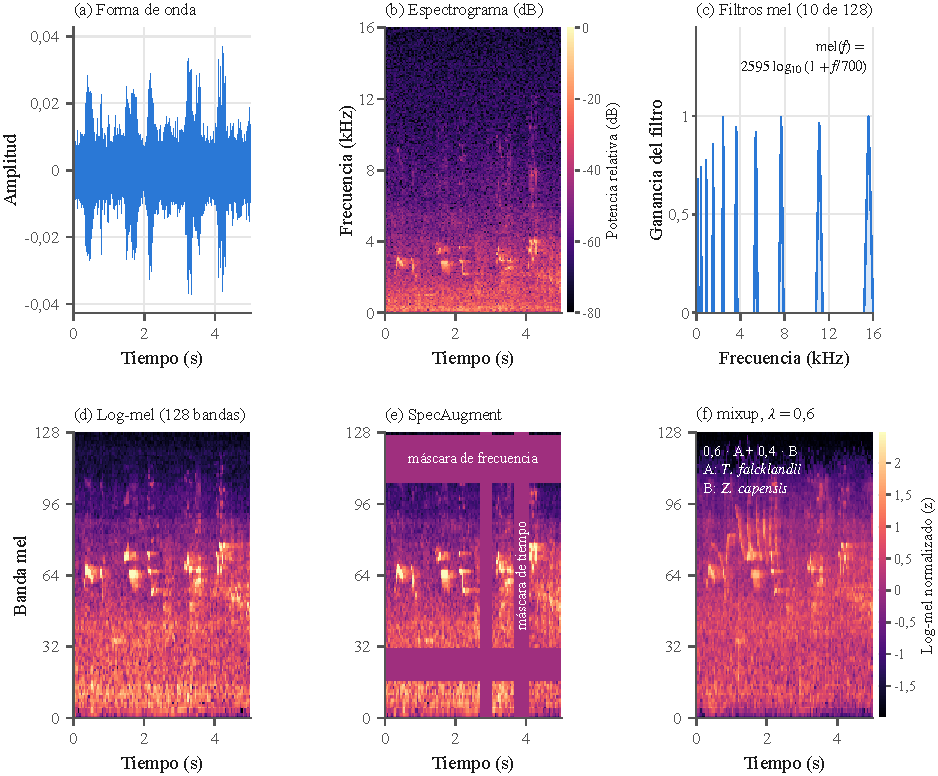
\includegraphics[width=\textwidth]{fig_representacion_audio}}{\fbox{figura pendiente}}
  \caption{Representación de entrada del clasificador de cantos para
  una ventana de \SI{5}{\second} de zorzal (\textit{Turdus falcklandii},
  XC954086): (a) forma de onda; (b) espectrograma de potencia; (c) diez de
  los 128 filtros del banco mel; (d) espectrograma log-mel de $128\times501$
  que recibe la CNN; (e) SpecAugment y (f) \textit{mixup} con una ventana
  de chincol, las dos aumentaciones de entrenamiento.}
  \label{fig:representacion-audio}
\end{figure}

\begin{figure}[H]
  \centering
  \resizebox{\textwidth}{!}{%
  \begin{tikzpicture}[
    node distance=6mm,
    paso/.style={draw, rounded corners, align=center, minimum height=9mm,
                 minimum width=23mm, font=\small, fill=black!5},
    aug/.style={paso, fill=miaamarillo!30},
    mod/.style={paso, fill=pucazul!15},
    flecha/.style={-{Latex[length=2mm]}, thick}]
    \node[paso] (a) {Audio\\Xeno-canto};
    \node[paso, right=of a] (b) {Mono,\\\SI{32}{kHz}};
    \node[paso, right=of b] (c) {Ventanas\\de \SI{5}{s}};
    \node[paso, right=of c] (d) {STFT +\\banco mel};
    \node[paso, right=of d] (e) {$\log(\cdot)$,\\estandarizar};
    \node[aug, below=of e] (f) {SpecAugment,\\mixup, ruido};
    \node[mod, right=of e] (g) {CNN};
    \node[paso, right=of g] (h) {Promedio\\ventanas};
    \draw[flecha] (a)--(b); \draw[flecha] (b)--(c); \draw[flecha] (c)--(d);
    \draw[flecha] (d)--(e); \draw[flecha] (e)--(g); \draw[flecha] (g)--(h);
    \draw[flecha, dashed] (e)--(f); \draw[flecha, dashed] (f)-|(g);
    \node[below=1mm of f, font=\scriptsize] {(solo en entrenamiento)};
  \end{tikzpicture}}
  \caption{Pipeline de procesamiento de audio de la CNN, desde la grabación
  original hasta la predicción a nivel de grabación. El AST sigue el mismo
  esquema con ventanas de \SI{10}{\second} remuestreadas a
  \SI{16}{\kilo\hertz} y su propio banco de filtros.}
  \label{fig:pipeline-audio}
\end{figure}

%-----------------------------------------------------------------------
\section{Protocolos de inferencia: ventanas, agregación y TTA}\label{sec:teoria-inferencia}

Las redes convolucionales con capa densa necesitan una entrada de tamaño
fijo, pero las grabaciones duran desde un segundo hasta varios minutos. Por
eso el modelo clasifica \emph{ventanas} de duración fija (\SI{5}{\second} en
la CNN, \SI{10}{\second} en el AST), y la predicción de una grabación se
obtiene recolectando y agregando las predicciones de sus ventanas, cuidando
que la evaluación se haga a nivel de grabación y no de ventana. Si una
grabación produce $W$ ventanas
$x^{(1)}, \dots, x^{(W)}$, la regla de agregación usada es el promedio de
probabilidades seguido del máximo \citep[pp.~26, 30]{virtanen2018casse}:
\begin{equation}
  \bar{p}_k = \frac{1}{W} \sum_{w=1}^{W} p(\mathcal{C}_k \mid x^{(w)}),
  \qquad \hat{y} = \argmax_k \bar{p}_k.
  \label{eq:agregacion}
\end{equation}
El promedio diluye las ventanas sin vocalización o con ruido entre las que sí
contienen al ave, lo que lo hace robusto a la anotación débil de Xeno-canto,
donde la especie está etiquetada para la grabación completa pero no para
cada instante (\secref{sec:rel-audio}). En esta tesis se reportan dos
protocolos: \emph{ventana única}, que clasifica solo la ventana central
($W = 1$), y \emph{agregado}, con hasta $W = 12$ ventanas de \SI{5}{\second}
equiespaciadas que cubren la grabación en la CNN, y hasta $W = 8$ de
\SI{10}{\second} en el AST (\figref{fig:ventanas-tta}a).

Para la imagen el análogo es la \emph{aumentación en tiempo de prueba}
(TTA): en lugar de clasificar un solo recorte central de la fotografía, se
clasifican diez vistas (los recortes de las cuatro esquinas y del centro, y
sus reflejos horizontales) y se promedian las probabilidades con la misma
Ecuación~\ref{eq:agregacion} (\figref{fig:ventanas-tta}b). Es la aumentación
de datos aplicada en inferencia: suaviza errores debidos al encuadre a cambio
de diez pasadas por el modelo.

\begin{figure}[!htb]
  \centering
  \IfFileExists{figuras/tikz_ventanas_tta.tex}{\fitwidth{\begin{tikzpicture}[x=1mm, y=1mm, font=\footnotesize,
    bloque/.style={draw, rounded corners, align=center, minimum height=9mm,
                   minimum width=24mm, font=\footnotesize, inner xsep=1mm},
    modelo/.style={bloque, fill=miaamarillo!30},
    proc/.style={bloque, fill=black!5, minimum width=26mm},
    salida/.style={bloque, fill=green!12, minimum width=16mm},
    flecha/.style={-{Latex[length=2mm]}, thick},
    etiq/.style={font=\scriptsize, align=center, inner sep=0.3mm},
    % pila de K vectores de probabilidad (icono)
    pics/probvec/.style={code={
      \foreach \d in {2.0,1.0} {\draw[fill=white, thin] (\d,\d) rectangle ++(9,6);}
      \draw[fill=white, thin] (0,0) rectangle (9,6);
      \foreach \bx/\bh in {0.9/1.2, 2.2/0.7, 3.5/4.6, 4.8/1.0, 6.1/1.9, 7.4/0.8}
        {\fill[pucazul!80] (\bx,0.5) rectangle ++(1.0,\bh);}
    }}]

  % ================= (a) AUDIO =================
  \node[anchor=west, inner sep=0] at (0,7.5)
    {\textbf{(a)} Audio: grabación de \SI{45}{s} a \SI{32}{kHz}};
  % barra de la grabación (45 mm = 45 s) con forma de onda estilizada
  \begin{scope}
    \draw[fill=pucazul!15, thin, rounded corners=0.8mm] (0,-3.5) rectangle (45,3.5);
    \clip (0,-3.5) rectangle (45,3.5);
    \draw[pucazul!60!black, line width=0.3pt]
      plot[domain=0:45, samples=320, smooth]
      (\x, {(0.22 + 2.7/(1+((\x-10)/2.2)^2) + 2.2/(1+((\x-24)/1.8)^2)
            + 2.0/(1+((\x-37)/1.6)^2)) * (0.7+0.3*sin(\x*73)) * sin(\x*300)});
  \end{scope}
  % K = 9 ventanas contiguas de 5 s (5 mm cada una)
  \foreach \i in {0,...,8} {
    \draw[fill=black!5, thin] ({\i*5},-8) rectangle ({\i*5+5},-4.5);
  }
  \draw[fill=miaamarillo!30, thick] (20,-8) rectangle (25,-4.5);
  \node[etiq, anchor=north west, align=left] at (0,-9.3)
    {$W=9$ ventanas de \SI{5}{s}, equiespaciadas ($W\le 12$)\\
     amarillo: \emph{ventana única} (central)};

  % pipeline (a), centrado en y=-2
  % llave: cada una de las K ventanas (no la grabación entera) entra a la CNN
  \draw[decorate, decoration={brace, amplitude=1.2mm}, thin] (46,3.5) -- (46,-8);
  \node[modelo] (cnn) at (72.5,-2) {CNN de audio\\EfficientNet-B0\\+ softmax};
  \draw[flecha] (48.2,-2.25) -- (cnn.west |- 0,-2.25)
    node[midway, above=0.4mm, etiq] {log-mel}
    node[midway, below=0.4mm, etiq] {$128{\times}501$};
  \pic at (88,-6.5) {probvec};
  \node[etiq, anchor=north] at (93.5,-7.6) {$W$ vectores\\$p^{(w)}\in\mathbb{R}^{55}$};
  \draw[flecha] (cnn.east) -- (87.6,-2);
  \node[proc] (prom) at (117.5,-2) {Promedio\\$\bar{p}=\frac{1}{W}\sum_{w} p^{(w)}$};
  \draw[flecha] (100.4,-2) -- (prom.west);
  \node[salida] (esp) at (149,-2) {Especie\\$\hat{y}$};
  \draw[flecha] (prom.east) -- (esp.west) node[midway, above=0.4mm, etiq] {$\arg\max$};

  % ================= (b) IMAGEN =================
  \node[anchor=west, inner sep=0] at (0,-23)
    {\textbf{(b)} Imagen: fotografía redimensionada (lado menor a \SI{441}{px})};
  % fotografía real del corpus (chucao, iNaturalist, CC BY-NC 4.0), recortada a 28 x 21 mm
  \begin{scope}
    \clip (8,-46.5) rectangle (36,-25.5);
    \node[inner sep=0] at (22,-36) {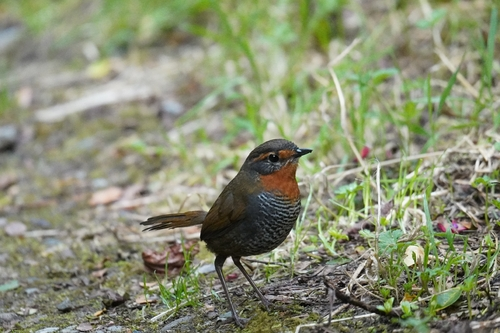
\includegraphics[height=21mm]{fig_tta_foto.jpg}};
  \end{scope}
  \draw[thin, black!40] (8,-46.5) rectangle (36,-25.5);
  % 4 recortes de esquina (azul, discontinuo): cuadrados de 15 x 15 mm, solapados
  \foreach \px/\py in {8/-25.5, 21/-25.5, 8/-31.5, 21/-31.5} {
    \draw[pucazul!70!black, dash pattern=on 1.2pt off 0.9pt, line width=0.5pt]
      (\px,\py) rectangle ++(15,-15);
  }
  % recorte central (amarillo, continuo), cuadrado de 15 x 15 mm
  \draw[miaamarillo!80!black, thick] (14.5,-28.5) rectangle ++(15,-15);
  \node[etiq, anchor=north west, align=left] at (0,-47.8)
    {5 recortes de $384{\times}384$ px: 4 esquinas + centro\\
     amarillo: \emph{recorte central} (1 vista)};

  % pipeline (b), centrado en y=-36
  \node[modelo] (b3) at (72.5,-36) {CNN de imagen\\EfficientNet-B3\\+ softmax};
  \draw[flecha] (36.4,-36) -- (b3.west)
    node[midway, above=0.4mm, etiq] {$\times 2$ volteo\\horizontal}
    node[midway, below=0.4mm, etiq] {$= 10$ vistas};
  \pic at (88,-40.5) {probvec};
  \node[etiq, anchor=north] at (93.5,-41.6) {10 vectores\\$p^{(v)}\in\mathbb{R}^{53}$};
  \draw[flecha] (b3.east) -- (87.6,-36);
  \node[proc] (promb) at (117.5,-36) {Promedio (TTA)\\$\bar{p}=\frac{1}{10}\sum_{v} p^{(v)}$};
  \draw[flecha] (100.4,-36) -- (promb.west);
  \node[salida] (espb) at (149,-36) {Especie\\$\hat{y}$};
  \draw[flecha] (promb.east) -- (espb.west) node[midway, above=0.4mm, etiq] {$\arg\max$};
\end{tikzpicture}
}}{\fbox{figura pendiente}}
  \caption{Protocolos de inferencia. (a) Audio: la grabación se divide en
  ventanas de \SI{5}{\second}, cada una pasa por la CNN y las probabilidades
  se promedian (Ecuación~\ref{eq:agregacion}); la \emph{ventana única} usa
  solo la central (en amarillo). (b) Imagen: cinco recortes de $384\times384$
  y sus volteos horizontales forman las diez vistas de la TTA; el
  \emph{recorte central} usa una sola (en amarillo). Fotografía de chucao de
  pmarinaraya (iNaturalist, CC BY-NC 4.0).}
  \label{fig:ventanas-tta}
\end{figure}

%-----------------------------------------------------------------------
\section{Fusión multimodal}\label{sec:teoria-fusion}

Sea $\mathcal{Y} = \{1, \dots, K\}$ el conjunto de especies. Cada observación
consiste en una señal de audio $x^{(a)}$ y/o una imagen $x^{(v)}$, con
etiqueta $y \in \mathcal{Y}$. Se entrenan dos clasificadores independientes,
$f_a$ y $f_v$, cada uno con su propia red y su propio conjunto de datos, que
producen las probabilidades $p_a(k \mid x^{(a)})$ y $p_v(k \mid x^{(v)})$ con
la Ecuación~\ref{eq:softmax}. Las tres formas de combinar las modalidades
\citep{baltrusaitis2019multimodal} se distinguen por el nivel en que ocurre
la combinación (\figref{fig:fusion-estrategias}).

\begin{itemize}[leftmargin=*, itemsep=2pt]
  \item \textbf{\textit{Early fusion}.} Se concatenan las representaciones
        internas de ambas ramas (sus \textit{embeddings} $\mathbf{h}_a \in
        \mathbb{R}^{1280}$ y $\mathbf{h}_v \in \mathbb{R}^{1536}$) y un único
        clasificador $g$ decide: $\hat{y} = \argmax_k g([\mathbf{h}_a;
        \mathbf{h}_v])_k$. Puede modelar interacciones entre modalidades,
        pero exige que ambas estén presentes.
  \item \textbf{\textit{Intermediate fusion}.} Cada \textit{embedding} pasa
        primero por una proyección propia a un espacio común de 256
        dimensiones y la concatenación de las proyecciones alimenta el
        clasificador. Agrega parámetros que deben aprenderse de los datos
        emparejados.
  \item \textbf{\textit{Late fusion}.} Cada rama decide por su cuenta y se
        combinan las probabilidades con una media ponderada por $\alpha \in
        [0, 1]$:
        \begin{equation}
          \hat{y} = \argmax_{k \in \mathcal{Y}} \;
          \alpha\, p_a(k \mid x^{(a)}) + (1-\alpha)\, p_v(k \mid x^{(v)}).
          \label{eq:fusion}
        \end{equation}
        Si falta una modalidad, $\hat{y}$ se obtiene de la otra, lo que hace
        al sistema robusto a modalidades faltantes y permite entrenar cada
        rama con datos no emparejados. Una alternativa es la media
        geométrica, $\propto p_a^{\alpha}\, p_v^{1-\alpha}$ (un producto de
        expertos). Con $\alpha = 1/2$ y un prior uniforme sobre las especies
        equivale, salvo normalización, a la combinación \textit{naive Bayes}
        $p(\mathcal{C}_k \mid x^{(a)})\, p(\mathcal{C}_k \mid x^{(v)}) /
        p(\mathcal{C}_k)$, que supone las dos modalidades condicionalmente
        independientes dada la especie \citep[pp.~146--147]{bishop2024deep}.
        Penaliza más a las clases que una modalidad descarta con seguridad.
\end{itemize}

\begin{figure}[!htb]
  \centering
  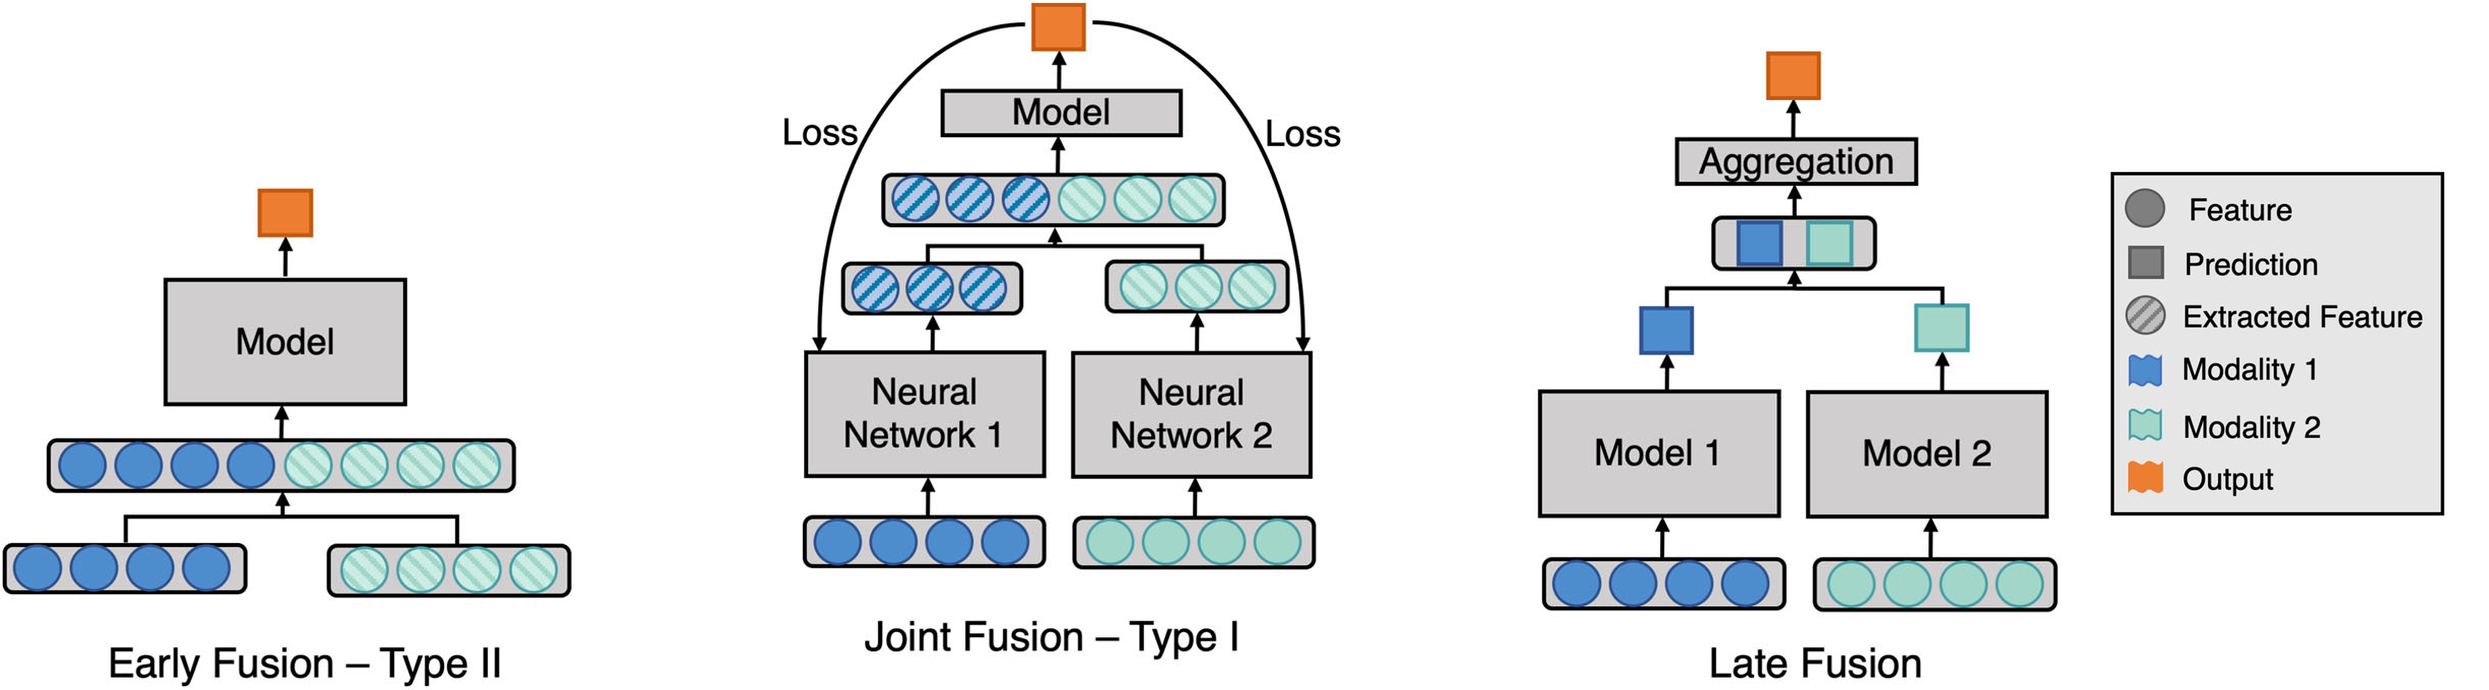
\includegraphics[width=\textwidth]{fig_fusion_huang2020.png}
  \caption{Estrategias de fusión multimodal: \textit{early fusion}
  (se concatenan las características extraídas de cada modalidad),
  \textit{joint fusion}, que corresponde a la \textit{intermediate fusion}
  de esta tesis (cada modalidad pasa por su propia red antes de
  concatenarse), y \textit{late fusion} (cada modalidad predice por separado
  y las predicciones se agregan). Los subtipos I y II distinguen si las
  características de entrada son crudas o extraídas. Tomada de
  \citet{huang2020fusion}, CC BY 4.0.}
  \label{fig:fusion-estrategias}
\end{figure}

\textbf{Evaluación con fuentes no emparejadas.} Las grabaciones de
Xeno-canto y las fotografías de iNaturalist no corresponden a los mismos
individuos, de modo que no existen pares naturales de audio e imagen. Para
evaluar la fusión se construyen pares sintéticos: cada grabación del
conjunto de prueba de audio se empareja al azar con una fotografía del
conjunto de prueba de imagen de la misma especie, repitiendo el
emparejamiento varias veces y reportando media y desviación estándar de las
métricas. Este protocolo mide la ganancia de combinar evidencia de ambas
modalidades, que es el escenario de uso previsto (un observador que dispone
de una grabación y una fotografía de la misma ave), pero no captura
correlaciones entre el canto y la apariencia de un mismo individuo. Esta
limitación se declara en el análisis de resultados.

%-----------------------------------------------------------------------
\section{Modelos de distribución de especies}\label{sec:teoria-sdm}

\subsection{Qué modela un modelo de distribución}

Un modelo de distribución de especies (SDM, o modelo de idoneidad de
hábitat) relaciona empíricamente las observaciones de una especie con las
condiciones ambientales de los sitios donde se la observó, y proyecta esa
relación a todo el territorio para estimar dónde podría estar
\citep[p.~11]{guisan2017hsdm}. Lo que captura es el \emph{nicho realizado}:
el conjunto de condiciones (temperatura, precipitación, vegetación,
altitud) en que la especie efectivamente se encuentra, una vez descontadas
la competencia y la historia, que es lo único observable con datos de campo
\citep[pp.~32, 36]{guisan2017hsdm}. El modelo supone que la especie está en
pseudoequilibrio con su ambiente y que la muestra cubre los ambientes que
ocupa. Por ser correlativo, apoya hipótesis pero no las prueba
\citep[pp.~46, 53]{guisan2017hsdm}. Formalmente, para cada especie $k$ se
dispone de presencias $\mathcal{P}_k = \{(s_i, t_i)\}$, con $s_i$ la
ubicación y $t_i$ la fecha, y cada punto se describe con un vector de
covariables $\mathbf{c}(s, t) \in \mathbb{R}^d$: temperatura media anual y
precipitación anual de WorldClim, elevación, NDVI y la codificación cíclica
del mes, $(\sin 2\pi t/12, \cos 2\pi t/12)$, que deja diciembre y enero
contiguos. El NDVI (índice de vegetación de diferencia normalizada) mide el
``verdor'' a partir de la luz que refleja la superficie en dos bandas del
espectro \citep{tucker1979ndvi}:
\begin{equation}
  \mathrm{NDVI} = \frac{\rho_{\mathrm{NIR}} - \rho_{\mathrm{Red}}}{\rho_{\mathrm{NIR}} + \rho_{\mathrm{Red}}},
  \label{eq:ndvi}
\end{equation}
donde $\rho_{\mathrm{NIR}}$ y $\rho_{\mathrm{Red}}$ son las \emph{reflectancias}
(fracción de la luz incidente que la superficie devuelve) en el infrarrojo
cercano y en el rojo. La vegetación verde refleja mucho infrarrojo y absorbe
el rojo, así que su NDVI se acerca a uno, mientras que el suelo desnudo, el
agua y la nieve dan valores cercanos a cero o negativos. Índices como este
``realzan'' una señal que las bandas por separado ocultan
\citep[p.~98]{guisan2017hsdm}.

\subsection{Datos de solo presencia y pseudoausencias}

Los registros de ciencia ciudadana son de \emph{solo presencia}: dicen dónde
se vio a la especie, nunca dónde se la buscó sin éxito. Un modelo que
contraste presencias con ausencias necesita entonces puntos de contraste
artificiales, los \emph{puntos de fondo} o \emph{pseudoausencias}, que
representan las condiciones ambientales disponibles en el territorio
\citep[pp.~131--134]{guisan2017hsdm}. La opción con menos supuestos es
muestrearlos al azar por toda el área de estudio. Pero los datos
oportunistas no se recogen al azar: se agrupan en zonas accesibles y a lo
largo de las vías de comunicación \citep[p.~56]{guisan2017hsdm}, y ese
sesgo de GBIF ha crecido con el tiempo. Con
un fondo uniforme el modelo aprende dónde hay observadores, no dónde hay
hábitat. El método del \emph{grupo objetivo} corrige el sesgo tomando como
pseudoausencias los registros de otras especies del mismo grupo (aquí, las
demás aves del conjunto), porque esos registros comparten exactamente el
esfuerzo de observación de las presencias \citep{phillips2009bias}. La
\figref{fig:fondo-objetivo} muestra la diferencia con los datos de esta
tesis.

\begin{figure}[!htb]
  \centering
  \IfFileExists{figuras/fig_fondo_objetivo.pdf}{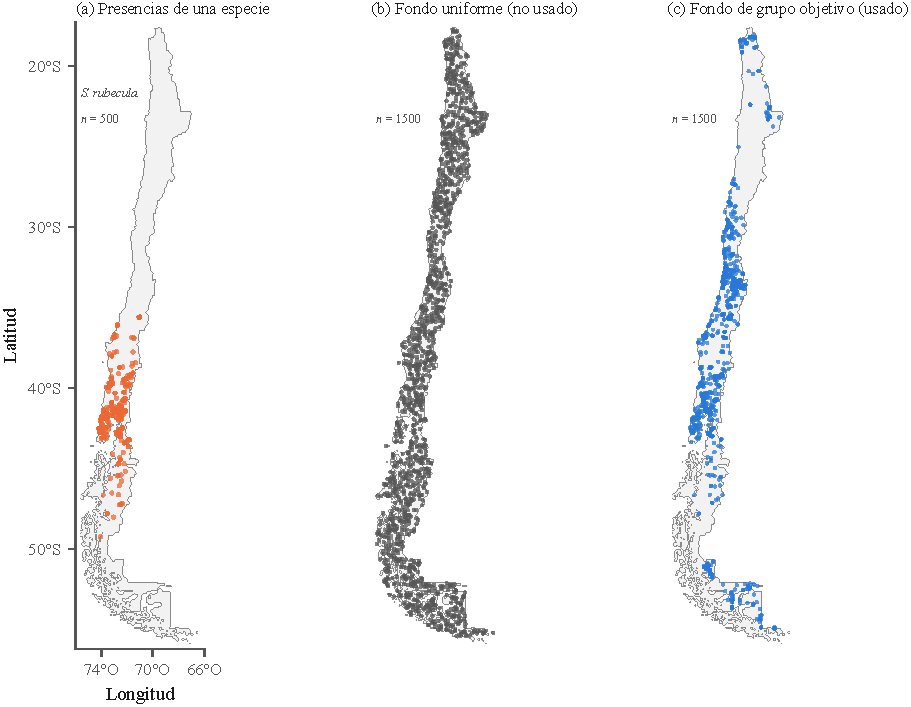
\includegraphics[width=\textwidth]{fig_fondo_objetivo}}{\fbox{figura pendiente}}
  \caption{Presencias y pseudoausencias del modelo de distribución:
  (a) 500 registros de chucao (\textit{Scelorchilus rubecula}); (b) fondo
  uniforme sobre Chile continental, descartado; (c) fondo de grupo objetivo,
  tomado de los avistamientos de las demás aves del conjunto, que reproduce
  la geografía del esfuerzo de observación y es el que usa la tesis.}
  \label{fig:fondo-objetivo}
\end{figure}

\subsection{MaxEnt y la regresión logística}

MaxEnt es el método de referencia para datos de solo presencia. Su idea: de
todas las distribuciones de probabilidad sobre el territorio compatibles con
lo observado, elegir la de máxima entropía, la más ``neutra''
\citep[p.~217]{guisan2017hsdm}. En la formulación de
\citet{elith2011maxent}, si $f(\mathbf{c})$ es la densidad de las condiciones
ambientales en el territorio (estimada con los puntos de fondo) y
$f_1(\mathbf{c})$ la densidad en los sitios de presencia, MaxEnt estima el
cociente $f_1(\mathbf{c})/f(\mathbf{c})$ buscando la $f_1$ más cercana a $f$ en
entropía relativa, sujeta a que los promedios de las covariables bajo $f_1$
coincidan con los observados en las presencias. La solución tiene forma
exponencial en una
combinación lineal de \emph{features} $h(\mathbf{c})$ de las covariables
(lineales, cuadráticas, de umbral, etc.) \citep{phillips2006maxent}:
\begin{equation}
  \frac{f_1(\mathbf{c})}{f(\mathbf{c})} = \exp\!\big(\eta(\mathbf{c})\big),
  \qquad \eta(\mathbf{c}) = \beta_0 + \boldsymbol{\beta}^{\mathrm{T}} h(\mathbf{c}),
  \label{eq:maxent}
\end{equation}
ajustada maximizando una verosimilitud penalizada, porque sin
regularización el modelo sobreajusta \citep[p.~219]{guisan2017hsdm}. Esta
forma es la de un modelo lineal generalizado: en el límite de un fondo
grande, contrastar presencias con el fondo mediante una regresión logística
penalizada estima las mismas pendientes $\boldsymbol{\beta}$ (el intercepto
difiere y depende del número de puntos de fondo)
\citep{fithian2013equivalence}. Por eso el \textit{baseline} MaxEnt de esta
tesis se implementa como una regresión logística con \textit{features}
lineales y cuadráticas y penalización L2 (la implementación original de
MaxEnt usa L1):
\begin{equation}
  P(y = 1 \mid \mathbf{c}) = \sigma\!\big(\mathbf{w}^{\mathrm{T}} h(\mathbf{c}) + b\big),
  \qquad \sigma(a) = \frac{1}{1 + e^{-a}},
  \label{eq:logistica}
\end{equation}
donde $\sigma$ es la función logística, que convierte el predictor lineal
(no acotado) en una probabilidad \citep[pp.~165--167]{guisan2017hsdm}. Los
términos cuadráticos producen las respuestas unimodales típicas de las
especies, que rinden mejor cerca de un óptimo ambiental y peor a ambos
lados. La ventaja de este modelo es su
interpretabilidad: cada coeficiente dice cómo cambia la probabilidad de
presencia con una covariable.

\subsection{Árboles de decisión, Random Forest y gradient boosting}

Un \emph{árbol de clasificación} divide los datos repetidamente en dos
grupos según una regla sobre una sola covariable (``NDVI $< 0{,}4$'',
``elevación $> \SI{1200}{\metre}$''), eligiendo en cada nodo la división que
mejor separa presencias de ausencias. Cada hoja guarda la proporción de
presencias que llegan a ella, que es su probabilidad predicha
\citep[p.~190]{guisan2017hsdm}. En la implementación usada, la impureza de
un nodo se mide con el índice de Gini, $G = 1 - p_{\mathrm{pres}}^2 -
p_{\mathrm{aus}}^2$, con $p_{\mathrm{pres}}$ y $p_{\mathrm{aus}}$ las
proporciones de presencias y ausencias en el nodo, y cada división minimiza la impureza ponderada de los dos hijos. El árbol no asume
ninguna forma de respuesta y captura interacciones, pero ajustar un solo
árbol es una operación de alta varianza: pequeños cambios en los datos
producen árboles muy distintos \citep[pp.~194, 203]{guisan2017hsdm}. Los
\emph{ensambles} corrigen eso combinando muchos árboles
(\figref{fig:arboles}).

\begin{figure}[!htb]
  \centering
  \IfFileExists{figuras/tikz_arboles.tex}{\fitwidth{% Ensambles de árboles para el modelo de distribución: (a) Random Forest,
% (b) gradient boosting y (c) MaxEnt como regresión logística penalizada.
% Incluir con \input dentro de un entorno figure (ancho ~157 mm).
% Los tres árboles de (a) son esquemáticos: profundidad 2, reglas y
% probabilidades de hoja ilustrativas (no provienen de un modelo ajustado).
\begin{tikzpicture}[x=1mm, y=1mm, font=\footnotesize,
  caja/.style={draw, rounded corners=1.5pt, align=center, inner sep=2pt, line width=0.4pt},
  datos/.style={caja, fill=pucazul!15},
  proc/.style={caja, fill=black!5},
  modelo/.style={caja, fill=miaamarillo!30},
  salida/.style={caja, fill=green!12},
  regla/.style={modelo, font=\scriptsize, inner xsep=1.2pt, inner ysep=1.5pt, minimum height=4.5mm},
  hoja/.style={salida, circle, font=\scriptsize, inner sep=0.6pt, minimum size=5mm},
  flecha/.style={-{Latex[length=2mm]}, thick},
  flechafina/.style={-{Latex[length=1.5mm]}, semithick},
  rama/.style={semithick, black!60},
  sino/.style={font=\scriptsize, text=black!75, inner sep=0.3pt},
  etq/.style={font=\scriptsize, inner sep=0.8pt},
  titulo/.style={font=\footnotesize\bfseries, anchor=west, inner sep=0},
  pres/.style={circle, fill=pucazul, draw=pucazul!50!black, inner sep=0, minimum size=1.7mm},
  fondo/.style={circle, fill=white, draw=black!60, semithick, inner sep=0, minimum size=1.7mm},
  pics/minitree/.style={code={
      \node[modelo, minimum size=3mm, inner sep=0, rounded corners=1pt] (-r) at (0,0) {};
      \node[salida, circle, minimum size=2.4mm, inner sep=0] (-a) at (-3,-4.5) {};
      \node[salida, circle, minimum size=2.4mm, inner sep=0] (-b) at (3,-4.5) {};
      \draw[rama] (-r) -- (-a); \draw[rama] (-r) -- (-b);}}]

  % ======================= (a) Random Forest =======================
  \node[titulo] at (0,67) {(a) Random Forest: \mdseries bagging de árboles con selección aleatoria de covariables};
  \node[datos] (datos) at (62,60)
    {Conjunto de entrenamiento: presencias ($y{=}1$) y fondo de grupo objetivo ($y{=}0$)\\
     con 6 covariables: NDVI, temperatura, precipitación, elevación, sen/cos del mes};

  % muestras bootstrap
  \node[proc, font=\scriptsize] (b1) at (20,46.5)  {Muestra\\bootstrap 1};
  \node[proc, font=\scriptsize] (b2) at (65,46.5)  {Muestra\\bootstrap 2};
  \node[proc, font=\scriptsize] (b3) at (107,46.5) {Muestra\\bootstrap 3};
  \node[font=\footnotesize] at (128,46.5) {$\cdots$};
  \coordinate (bus) at ($(datos.south)+(0,-1.8)$);
  \draw[thick] (datos.south) -- (bus);
  \draw[thick] (bus -| b1.north) -- (bus -| b3.north);
  \draw[flecha] (bus -| b1.north) -- (b1.north);
  \draw[flecha] (bus -| b2.north) -- (b2.north);
  \draw[flecha] (bus -| b3.north) -- (b3.north);

  % ---- árbol 1 ----
  \node[regla] (r1)  at (20,36.5) {NDVI $<$ 0,4};
  \node[regla] (c11) at (9,28)  {elev. $>$ \SI{1200}{m}};
  \node[regla] (c12) at (31,28) {temp. $>$ \SI{12}{\celsius}};
  \node[hoja] (h11) at (3.5,20.5)  {0,10};
  \node[hoja] (h12) at (14.5,20.5) {0,35};
  \node[hoja] (h13) at (25.5,20.5) {0,80};
  \node[hoja] (h14) at (36.5,20.5) {0,45};
  \draw[rama] (r1) -- (c11) node[sino, pos=0.7, above left=-0.5pt] {sí};
  \draw[rama] (r1) -- (c12) node[sino, pos=0.7, above right=-0.5pt] {no};
  \draw[rama] (c11) -- (h11); \draw[rama] (c11) -- (h12);
  \draw[rama] (c12) -- (h13); \draw[rama] (c12) -- (h14);
  \node[font=\scriptsize] (t1) at (20,15.5) {$T_1(\mathbf{c})$};

  % ---- árbol 2 ---- (los árboles 2 y 3 van 3 mm a la derecha para que las
  % reglas de árboles vecinos no se toquen)
  \begin{scope}[xshift=3mm]
  \node[regla] (r2)  at (62,36.5) {temp. $>$ \SI{12}{\celsius}};
  \node[regla] (c21) at (51,28) {precip. $<$ \SI{300}{mm}};
  \node[regla] (c22) at (73,28) {sen(mes) $>$ 0};
  \node[hoja] (h21) at (45.5,20.5) {0,20};
  \node[hoja] (h22) at (56.5,20.5) {0,65};
  \node[hoja] (h23) at (67.5,20.5) {0,15};
  \node[hoja] (h24) at (78.5,20.5) {0,50};
  \draw[rama] (r2) -- (c21) node[sino, pos=0.7, above left=-0.5pt] {sí};
  \draw[rama] (r2) -- (c22) node[sino, pos=0.7, above right=-0.5pt] {no};
  \draw[rama] (c21) -- (h21); \draw[rama] (c21) -- (h22);
  \draw[rama] (c22) -- (h23); \draw[rama] (c22) -- (h24);
  \node[font=\scriptsize] (t2) at (62,15.5) {$T_2(\mathbf{c})$};
  \end{scope}

  % ---- árbol 3 ----
  \begin{scope}[xshift=3mm]
  \node[regla] (r3)  at (104,36.5) {elev. $>$ \SI{1200}{m}};
  \node[regla] (c31) at (93,28)  {NDVI $<$ 0,4};
  \node[regla] (c32) at (115,28) {precip. $>$ \SI{800}{mm}};
  \node[hoja] (h31) at (87.5,20.5)  {0,05};
  \node[hoja] (h32) at (98.5,20.5)  {0,40};
  \node[hoja] (h33) at (109.5,20.5) {0,70};
  \node[hoja] (h34) at (120.5,20.5) {0,30};
  \draw[rama] (r3) -- (c31) node[sino, pos=0.7, above left=-0.5pt] {sí};
  \draw[rama] (r3) -- (c32) node[sino, pos=0.7, above right=-0.5pt] {no};
  \draw[rama] (c31) -- (h31); \draw[rama] (c31) -- (h32);
  \draw[rama] (c32) -- (h33); \draw[rama] (c32) -- (h34);
  \node[font=\scriptsize] (t3) at (104,15.5) {$T_3(\mathbf{c})$};
  \end{scope}

  \draw[flecha] (b1) -- (r1); \draw[flecha] (b2) -- (r2); \draw[flecha] (b3) -- (r3);


  % promedio
  \node[salida] (prom) at (65,5.5)
    {Promedio de los $B$ árboles: \; $p(\mathbf{c}) = \frac{1}{B}\sum_{b=1}^{B} T_b(\mathbf{c})$};
  \draw[flecha] (t1.south) -- ++(0,-2.5) -| ([xshift=-14mm]prom.north);
  \draw[flecha] (t2.south) -- (prom.north);
  \draw[flecha] (t3.south) -- ++(0,-2.5) -| ([xshift=14mm]prom.north);

  % separadores
  \draw[black!30, dashed] (0,-1) -- (157,-1);
  \draw[black!30, dashed] (107.5,-3) -- (107.5,-56);

  % ======================= (b) Gradient boosting =======================
  \node[titulo] at (0,-5) {(b) Gradient boosting: \mdseries árboles secuenciales sobre el residuo};
  \node[proc] (F0) at (8,-40) {$F_0(\mathbf{c})$\\[-2pt]{\scriptsize constante}};
  \node[proc] (F1) at (30,-40) {$F_1(\mathbf{c})$};
  \node[proc] (F2) at (52,-40) {$F_2(\mathbf{c})$};
  \node[proc] (F3) at (74,-40) {$F_3(\mathbf{c})$};
  \node[inner sep=0.5pt] (Fd) at (86,-40) {$\cdots$};
  \node[salida] (FM) at (97,-40) {$F_J(\mathbf{c})$};
  \node[font=\scriptsize, anchor=north, inner sep=1pt] at ([xshift=-1mm]FM.south) {$p(\mathbf{c})=\sigma\big(F_J(\mathbf{c})\big)$};
  \draw[flecha] (F0) -- (F1); \draw[flecha] (F1) -- (F2); \draw[flecha] (F2) -- (F3);
  \draw[flecha] (F3) -- (Fd); \draw[flecha] (Fd) -- (FM);

  \pic (g1) at (19,-23) {minitree};
  \pic (g2) at (41,-23) {minitree};
  \pic (g3) at (63,-23) {minitree};
  \node[font=\scriptsize] at (19,-17.5) {$T_1(\mathbf{c})$};
  \node[font=\scriptsize] at (41,-17.5) {$T_2(\mathbf{c})$};
  \node[font=\scriptsize] at (63,-17.5) {$T_3(\mathbf{c})$};

  \draw[flechafina, dashed] (F0.north) -- (g1-a.south west)
        node[etq, pos=0.62, left] {$r_1$};
  \draw[flechafina] (g1-b.south east) -- (F1.north)
        node[etq, pos=0.3, right] {$\nu T_1$};
  \draw[flechafina, dashed] (F1.north) -- (g2-a.south west)
        node[etq, pos=0.62, left] {$r_2$};
  \draw[flechafina] (g2-b.south east) -- (F2.north)
        node[etq, pos=0.3, right] {$\nu T_2$};
  \draw[flechafina, dashed] (F2.north) -- (g3-a.south west)
        node[etq, pos=0.62, left] {$r_3$};
  \draw[flechafina] (g3-b.south east) -- (F3.north)
        node[etq, pos=0.3, right] {$\nu T_3$};

  \draw[flechafina, dashed] (2,-48.5) -- (7,-48.5);
  \node[anchor=west, font=\scriptsize] at (7.5,-48.5)
    {pseudorresiduo $r_m = y - \sigma\big(F_{m-1}(\mathbf{c})\big)$ que aprende el árbol $T_m$};
  \draw[flechafina] (2,-52) -- (7,-52);
  \node[anchor=west, font=\scriptsize] at (7.5,-52)
    {$F_m(\mathbf{c}) = F_{m-1}(\mathbf{c}) + \nu\,T_m(\mathbf{c})$, \; $\nu = 0{,}05$, \; $J = 300$};

  % ======================= (c) MaxEnt / regresión logística =======================
  \node[titulo] at (110,-5) {(c) MaxEnt: \mdseries regresión logística};
  % leyenda
  \node[pres] at (118,-10.5) {};
  \node[anchor=west, font=\scriptsize, inner sep=1pt] at (119.5,-10.5) {presencia};
  \node[fondo] at (139,-10.5) {};
  \node[anchor=west, font=\scriptsize, inner sep=1pt] at (140.5,-10.5) {fondo};
  % región de presencia (lado positivo de la frontera)
  \begin{scope}
    \clip (116,-46) rectangle (154,-14);
    \fill[pucazul!8] (116,-22.82) -- (154,-45.18) -- (154,-14) -- (116,-14) -- cycle;
  \end{scope}
  % ejes
  \draw[flechafina, black!70] (116,-46) -- (155,-46);
  \draw[flechafina, black!70] (116,-46) -- (116,-13);
  \node[font=\scriptsize] at (135.5,-48.3) {$h_1(\mathbf{c})$};
  \node[font=\scriptsize, rotate=90] at (113.3,-30) {$h_2(\mathbf{c})$};
  % frontera
  \draw[thick, pucazul!60!black] (116,-22.82) -- (154,-45.18)
    node[pos=0.22, above, sloped, font=\scriptsize, inner sep=0.8pt] {$\mathbf{w}^{\mathrm T} h(\mathbf{c}) + b = 0$};
  % presencias (una, (124,-32), queda del lado del fondo: error de clasificación)
  \foreach \p in {(126,-22),(132,-21),(138,-26),(144,-24),(148,-33),(141,-31),(135,-28),(150,-40),(131,-25),(146,-37),(124,-32)}
    \node[pres] at \p {};
  % fondo (uno, (139,-33), queda del lado de las presencias: error de clasificación)
  \foreach \p in {(119,-42),(123,-38),(128,-44),(133,-40),(120,-30),(126,-35),(137,-43),(142,-42),(131,-36),(139,-33),(147,-45)}
    \node[fondo] at \p {};
  \node[font=\scriptsize] at (135,-53) {$P(y{=}1 \mid \mathbf{c}) = \sigma\!\left(\mathbf{w}^{\mathrm T} h(\mathbf{c}) + b\right)$};
\end{tikzpicture}
}}{\fbox{figura pendiente}}
  \caption{Modelos de distribución basados en árboles y modelo lineal:
  (a) Random Forest promedia $B$ árboles entrenados sobre muestras
  \textit{bootstrap} (Ecuación~\ref{eq:rf}); (b) gradient boosting suma
  árboles ajustados secuencialmente al pseudorresiduo
  (Ecuación~\ref{eq:gbm}); (c) MaxEnt como regresión logística penalizada
  sobre las \textit{features} $h(\mathbf{c})$ (Ecuación~\ref{eq:logistica}).
  Esquemas propios a partir de \citet{breiman2001rf},
  \citet{friedman2001gbm} y \citet{elith2011maxent}.}
  \label{fig:arboles}
\end{figure}

\begin{itemize}[leftmargin=*, itemsep=2pt]
  \item \textbf{Random Forest} \citep{breiman2001rf}. Entrena $B$ árboles,
        cada uno sobre una muestra \textit{bootstrap} de los datos y eligiendo
        en cada nodo la mejor división entre un subconjunto aleatorio de
        $\sqrt{d}$ covariables, sin poda, y promedia sus probabilidades:
        \begin{equation}
          \hat{p}(\mathbf{c}) = \frac{1}{B} \sum_{b=1}^{B} T_b(\mathbf{c}).
          \label{eq:rf}
        \end{equation}
        El azar en los datos y en las variables descorrelaciona los árboles,
        y el promedio reduce drásticamente la varianza
        \citep[p.~278]{bishop2024deep}. Aquí $B = 300$.
  \item \textbf{Gradient boosting} \citep{friedman2001gbm}. Construye el
        modelo de forma secuencial: cada árbol pequeño $T_m$ se ajusta al
        gradiente negativo de la pérdida del conjunto anterior, es decir, a lo
        que todavía está mal modelado, y se suma con una tasa de aprendizaje
        $\nu$ que regula el peso de los árboles sucesivos:
        \begin{equation}
          F_m(\mathbf{c}) = F_{m-1}(\mathbf{c}) + \nu\, T_m(\mathbf{c}),
          \qquad m = 1, \dots, J, \qquad
          \hat{p}(\mathbf{c}) = \sigma\big(F_J(\mathbf{c})\big),
          \label{eq:gbm}
        \end{equation}
        con $F_0$ el logit de la proporción inicial de presencias. Los
        \textit{boosted regression trees} están entre los métodos de
        mejor desempeño en modelado de distribución \citep{elith2008brt,
        valavi2022benchmark}. Aquí $J = 300$ y $\nu = 0{,}05$.
\end{itemize}


\subsection{Red neuronal conjunta multiespecie}

Los SDM neuronales reemplazan las curvas de respuesta fijas de la regresión
por una red que aprende interacciones no lineales entre covariables
\citep{botella2018deepsdm, deneu2021cnn}. El modelo de esta tesis es un
perceptrón multicapa \emph{conjunto}: una única red para las 54 especies,
que recibe las seis covariables concatenadas con un vector aprendido de 8
dimensiones que identifica a la especie $k$ (su \textit{embedding}
$\mathbf{e}_k$),
\begin{equation}
  P(y_k = 1 \mid \mathbf{c}) = \sigma\!\Big( g_\theta\big([\mathbf{c};\, \mathbf{e}_k]\big) \Big),
  \label{eq:deepsdm}
\end{equation}
con $g_\theta$ una red de parámetros $\theta$ con dos capas ocultas de 64
unidades ReLU y \textit{dropout}, entrenada con la entropía cruzada binaria
ponderada por clase, de modo que presencias y fondo pesen lo mismo
(\figref{fig:mlp-sdm}). Compartir
la red entre especies transfiere información estadística de las especies
con muchos registros a las de pocos, como hacen los modelos de
\citet{cole2023sinr}. Sin capas ocultas, el modelo se reduce a una regresión logística con
pendientes compartidas entre especies y un intercepto por especie; el
\textit{baseline} MaxEnt de la Ecuación~\ref{eq:logistica} es el extremo
opuesto, con un modelo independiente por especie y \textit{features}
cuadráticas.

\begin{figure}[!htb]
  \centering
  \IfFileExists{figuras/tikz_mlp_sdm.tex}{\resizebox{0.80\textwidth}{!}{% Figura: red neuronal conjunta multiespecie para la distribución (SDM).
% Se incluye con \input dentro de un entorno figure. Unidades: mm.
% Notación de salida unificada con el capítulo 3: P(y_k = 1 | c).
\begin{tikzpicture}[
    x=1mm, y=1mm, font=\footnotesize,
    neurona/.style={circle, draw, thin, minimum size=4.4mm, inner sep=0pt},
    cov/.style={neurona, fill=pucazul!15},
    emb/.style={neurona, fill=miaamarillo!30},
    oculta/.style={neurona, fill=miaamarillo!30},
    logit/.style={neurona, fill=green!12, minimum size=5mm},
    caja/.style={draw, rounded corners, align=center, fill=green!12,
                 inner sep=3pt, minimum height=8mm},
    etiq/.style={align=center, font=\footnotesize},
    flecha/.style={-{Latex[length=2mm]}, thick},
    flechita/.style={-{Latex[length=1.5mm]}, semithick, pucgris},
    conexion/.style={black!30, line width=0.3pt},
    puntos/.style={inner sep=0pt}]

  % ---------- Entrada: seis covariables ----------
  \foreach \y/\n/\t in {27/c1/NDVI, 22/c2/Temperatura, 17/c3/Precipitación,
                        12/c4/Elevación, 7/c5/sen(mes), 2/c6/cos(mes)} {
    \node[cov] (\n) at (0,\y) {};
    \node[anchor=east, inner sep=1pt] at (-5,\y) {\t};
  }

  % ---------- Entrada: vector de embedding de la especie k ----------
  \node[emb] (e1) at (0,-4)  {};
  \node[emb] (e2) at (0,-9)  {};
  \node[puntos] at (0,-14) {$\vdots$};
  \node[emb] (e3) at (0,-19) {};

  % ---------- Tabla de embeddings (54 especies x 8 dimensiones) ----------
  % Esquema: 7 filas de 2 mm más una fila de puntos suspensivos (3 mm,
  % entre y=-16 e y=-19) que indica las filas omitidas; la fila k es la
  % cuarta (resaltada). Ocho columnas = ocho dimensiones del embedding.
  \fill[miaamarillo!30] (-25,-6)  rectangle (-9,-16);
  \fill[miaamarillo!30] (-25,-19) rectangle (-9,-23);
  \fill[miaamarillo]    (-25,-12) rectangle (-9,-14);
  \foreach \i in {1,...,7} {
    \draw[black!40, very thin] (-25+2*\i,-6)  -- (-25+2*\i,-16);
    \draw[black!40, very thin] (-25+2*\i,-19) -- (-25+2*\i,-23);
  }
  \foreach \yy in {-8,-10,-12,-14,-16,-19,-21} {
    \draw[black!40, very thin] (-25,\yy) -- (-9,\yy);
  }
  \draw[thin] (-25,-6) rectangle (-9,-23);
  \node[puntos, font=\scriptsize] at (-17,-17.5) {$\vdots$};
  \node[anchor=east, inner sep=1pt] at (-25.8,-13) {fila $k$};
  \node[etiq, anchor=north] at (-17,-24)
    {Tabla de embeddings\\$\mathbf{E}\in\mathbb{R}^{54\times 8}$ (aprendida)};
  % búsqueda de la fila k -> vector e_k
  \draw[flechita] (-9,-13) -- (e1.west);
  \draw[flechita] (-9,-13) -- (e2.west);
  \draw[flechita] (-9,-13) -- (e3.west);
  \node[font=\scriptsize, inner sep=0pt] at (-6.5,-19) {$\mathbf{e}_k$};

  % ---------- Capas ocultas (64 unidades cada una) ----------
  \foreach \y/\i in {25/1, 19/2, 13/3, 7/4, -5/5, -11/6, -17/7} {
    \node[oculta] (h1\i) at (24,\y) {};
    \node[oculta] (h2\i) at (48,\y) {};
  }
  \node[puntos] at (24,1) {$\vdots$};
  \node[puntos] at (48,1) {$\vdots$};

  % ---------- Salida ----------
  \node[logit] (z) at (70,4) {$z$};
  \node[caja] (p) at (102,4)
    {$P(y_k=1\mid\mathbf{c})=\sigma(z)$\\[1pt]$\sigma(z)=1/(1+e^{-z})$};
  \draw[flecha] (z) -- (p) node[midway, above, font=\scriptsize, inner sep=2pt] {sigmoide};

  % ---------- Conexiones densas y recuadro de concatenación ----------
  \begin{scope}[on background layer]
    \node[draw, dashed, rounded corners, fill=black!5, inner sep=1.5mm,
          fit=(c1)(e3)] (entrada) {};
    \foreach \a in {c1,c2,c3,c4,c5,c6,e1,e2,e3}
      \foreach \b in {1,...,7} \draw[conexion] (\a.east) -- (h1\b.west);
    \foreach \a in {1,...,7}
      \foreach \b in {1,...,7} \draw[conexion] (h1\a.east) -- (h2\b.west);
    \foreach \a in {1,...,7} \draw[conexion] (h2\a.east) -- (z.west);
  \end{scope}

  % ---------- Etiquetas de capa ----------
  \node[etiq, anchor=south] at (0,31.5)
    {Concatenación\\$\mathbf{x}=[\mathbf{c};\mathbf{e}_k]\in\mathbb{R}^{14}$};
  \node[etiq, anchor=south] at (24,31.5) {Capa oculta 1\\64 ReLU\\dropout 0,3};
  \node[etiq, anchor=south] at (48,31.5) {Capa oculta 2\\64 ReLU\\dropout 0,3};
  \node[etiq, anchor=south] at (70,31.5) {Salida\\1 logit};

  % ---------- Fórmulas ----------
  % Ancladas 3 mm más abajo que la etiqueta de la tabla para que no se
  % toquen cuando \onehalfspacing (preámbulo de la tesis) estira las
  % líneas de la etiqueta.
  \node[anchor=north] at (48,-35)
    {$\mathbf{h}_1=\mathrm{ReLU}(\mathbf{W}_1\mathbf{x}+\mathbf{b}_1)\qquad
      \mathbf{h}_2=\mathrm{ReLU}(\mathbf{W}_2\mathbf{h}_1+\mathbf{b}_2)\qquad
      z=\mathbf{w}_3^{\top}\mathbf{h}_2+b_3$};

  % ---------- Nota al pie ----------
  \node[font=\footnotesize\itshape, align=center] at (41,-45)
    {Una sola red para las 54 especies: las covariables comparten pesos
     y la especie entra como vector aprendido};
\end{tikzpicture}
}}{\fbox{figura pendiente}}
  \caption{Red neuronal conjunta multiespecie del modelo de distribución.
  Las seis covariables (azul) se concatenan con el \textit{embedding}
  aprendido de la especie (amarillo) y atraviesan dos capas ocultas de 64
  unidades hasta un logit cuya sigmoide es la probabilidad de presencia
  (Ecuación~\ref{eq:deepsdm}); todas las especies comparten las capas
  ocultas.}
  \label{fig:mlp-sdm}
\end{figure}

%-----------------------------------------------------------------------
\section{Métricas de evaluación}\label{sec:teoria-metricas}

\subsection{Matriz de confusión, \textit{accuracy} y F1}

Toda métrica de clasificación parte de contar, para cada clase $k$, cuatro
resultados al comparar la predicción con la verdad: verdaderos positivos
$\mathrm{TP}_k$ (muestras de la especie $k$ predichas como $k$), falsos
positivos $\mathrm{FP}_k$ (muestras de otra especie predichas como $k$),
falsos negativos $\mathrm{FN}_k$ (muestras de $k$ predichas como otra
especie) y verdaderos negativos $\mathrm{TN}_k$. La \emph{matriz de
confusión} de $K \times K$ tabula cuántas muestras de cada especie
verdadera (filas) se predijeron como cada especie (columnas). Su diagonal
son los aciertos y fuera de ella se ve qué especies se confunden con cuáles
\citep[pp.~147--148]{bishop2024deep}. Con $N$ muestras de prueba:
\begin{align}
  \mathrm{Accuracy} &= \frac{1}{N}\sum_{i=1}^{N} \mathbb{I}[\hat{y}_i = y_i], \label{eq:acc} \\
  \mathrm{F1}_{\mathrm{macro}} &= \frac{1}{K}\sum_{k=1}^{K}
    \frac{2\,\mathrm{TP}_k}{2\,\mathrm{TP}_k + \mathrm{FP}_k + \mathrm{FN}_k}, \label{eq:f1}
\end{align}
donde $\mathbb{I}[\cdot]$ vale uno si la condición se cumple y cero si no. La
\textit{accuracy} es la fracción de aciertos y pesa cada muestra por igual,
por lo que la dominan las clases frecuentes. Con clases raras puede ser alta
aunque el sistema no acierte ninguna de ellas. El F1 de una clase es la
media armónica de
su precisión ($\mathrm{TP}/(\mathrm{TP}+\mathrm{FP})$, qué fracción de lo
predicho como $k$ era realmente $k$) y su \textit{recall}
($\mathrm{TP}/(\mathrm{TP}+\mathrm{FN})$, qué fracción de las muestras de $k$
se recuperó), y el F1 \emph{macro} promedia el F1 de todas las clases por
igual, de modo que una especie amenazada con tres grabaciones de prueba pesa
tanto como una común con ocho \citep[pp.~170--171]{virtanen2018casse}. Por
eso es la métrica de selección de modelos de esta tesis y la que mejor
refleja el foco en las especies raras. También se reporta la
\textit{accuracy} top-5, que acepta la predicción si la especie correcta
está entre las cinco más probables, útil para un asistente que propone
candidatas.

\subsection{Curva ROC y AUC}

Las métricas anteriores dependen de una decisión (el argmax). Para evaluar
la calidad de las probabilidades sin fijar un umbral se usa la curva ROC:
para cada posible umbral sobre la probabilidad de la clase $k$ se calcula la
tasa de verdaderos positivos, $\mathrm{TPR} = \mathrm{TP}/(\mathrm{TP} +
\mathrm{FN})$ (la \emph{sensibilidad}), y la de falsos positivos,
$\mathrm{FPR} = \mathrm{FP}/(\mathrm{FP}+\mathrm{TN})$ (uno menos la
\emph{especificidad}), y se grafica una contra otra
\citep[p.~172]{virtanen2018casse}. Un clasificador perfecto pasa por la
esquina superior izquierda y uno aleatorio sigue la diagonal
(\figref{fig:roc}). El \emph{área bajo la curva} (AUC) resume toda la curva en
un número entre 0,5 (azar) y 1 (perfecto), y tiene una interpretación
probabilística: es la probabilidad de que el modelo asigne mayor puntaje a
un positivo elegido al azar que a un negativo elegido al azar
\citep{hanley1982auc}:
\begin{equation}
  \mathrm{AUC}_k = \frac{1}{n_k^{+}\, n_k^{-}} \sum_{i \in \text{pos}} \sum_{j \in \text{neg}}
  \Big(\mathbb{I}\big[p_k(\mathbf{x}_i) > p_k(\mathbf{x}_j)\big]
  + \tfrac{1}{2}\,\mathbb{I}\big[p_k(\mathbf{x}_i) = p_k(\mathbf{x}_j)\big]\Big),
  \label{eq:auc}
\end{equation}
donde $n_k^{+}$ y $n_k^{-}$ son el número de muestras positivas y negativas
de la clase $k$ y los empates cuentan medio. La ROC está definida para
problemas binarios. En clasificación multiclase se trata cada especie como
un problema binario (``esta especie frente a todas las demás'') y se
promedian las $K$ áreas, el AUC macro, $\frac{1}{K}\sum_k \mathrm{AUC}_k$. A diferencia de la
precisión, el AUC no cambia al agregar más negativos
\citep[pp.~173, 176]{virtanen2018casse}.

\begin{figure}[!htb]
  \centering
  \IfFileExists{figuras/fig_roc.pdf}{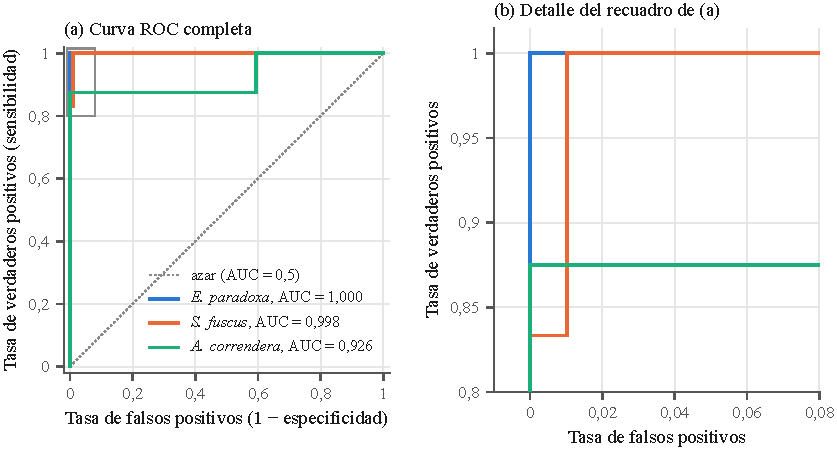
\includegraphics[width=\textwidth]{fig_roc}}{\fbox{figura pendiente}}
  \caption{Curvas ROC de la CNN de audio (prueba, protocolo agregado) para
  tres especies con al menos seis grabaciones de prueba: una con AUC igual
  a uno (\textit{Eugralla paradoxa}), la mediana (\textit{Scytalopus
  fuscus}, 0,998) y la de menor AUC (\textit{Anthus correndera}, 0,926). La
  diagonal es el clasificador al azar; el panel (b) amplía el recuadro de
  (a).}
  \label{fig:roc}
\end{figure}

En el modelo de distribución el AUC es la métrica estándar
\citep{valavi2022benchmark}: para cada especie compara las probabilidades
asignadas a las presencias de prueba con las de los puntos de fondo. Hay dos
salvedades. Como los puntos de fondo no son ausencias reales, el AUC mide la
capacidad de distinguir presencias del ambiente disponible, no de ausencias
verdaderas, y sus valores son relativos: solo permiten comparar modelos de
una misma especie en una misma área \citep[p.~265]{guisan2017hsdm}. Además,
es poco sensible al tamaño muestral y a la prevalencia, lo que lo vuelve
optimista \citep[p.~120]{guisan2017hsdm}, y depende de la extensión del
área de estudio \citep{lobo2008auc}. Por eso la tesis lo usa para comparar
métodos sobre los mismos datos, no como valor absoluto.

\subsection{Incertidumbre de las métricas}

Con conjuntos de prueba pequeños las métricas son ruidosas: una grabación
más o menos acertada cambia el F1 de una especie con tres muestras de 1,00 a
0,80, y dos errores lo bajan a 0,50. Esta tesis estima la incertidumbre con el \textit{bootstrap}
\citep{efron1993bootstrap}: se remuestrea el conjunto de prueba con
reemplazo $R$ veces, se recalcula la métrica en cada remuestra y los
percentiles 2,5 y 97,5 de esos valores forman el intervalo de confianza al
\SI{95}{\percent}. Para comparar dos modelos de distribución, que se evalúan
sobre las mismas especies, se usa el test de Wilcoxon de rangos con signo,
que contrasta si las diferencias de AUC por especie se distribuyen
simétricamente alrededor de cero sin suponer normalidad.

%-----------------------------------------------------------------------
\section{Autocorrelación espacial y validación por bloques}\label{sec:teoria-validacion}

\begin{figure}[!htb]
  \centering
  \IfFileExists{figuras/fig_blockcv.pdf}{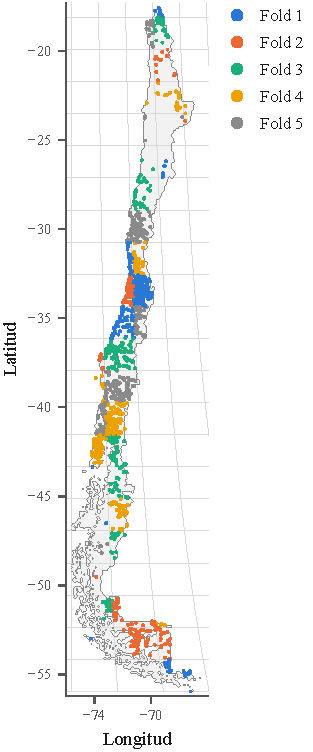
\includegraphics{fig_blockcv}}{\fbox{figura pendiente}}
  \caption{Partición espacial por bloques de \SI{200}{\kilo\metre} usada
  para validar los modelos de distribución: muestra de 8\,000 de los
  34\,926 puntos del conjunto del SDM, coloreados según el \textit{fold} de
  su bloque (46 bloques repartidos al azar en cinco \textit{folds} de tamaño
  equilibrado). Cada \textit{fold} de prueba contiene bloques completos
  ausentes del entrenamiento.}
  \label{fig:blockcv}
\end{figure}

La \figref{fig:blockcv} muestra la partición espacial que usa esta tesis;
esta sección explica por qué hace falta. Los datos ecológicos violan un
supuesto básico de la evaluación: las
observaciones cercanas no son independientes, porque comparten ambiente,
historia y, en ciencia ciudadana, observador. Esta \emph{autocorrelación
espacial} se mide con el semivariograma, que promedia las diferencias al
cuadrado entre pares de puntos separados por una distancia $d$:
\begin{equation}
  \gamma(d) = \frac{1}{2\,|N(d)|} \sum_{(i,j) \in N(d)} \big(z_i - z_j\big)^2,
  \label{eq:variograma}
\end{equation}
donde $N(d)$ son los pares a distancia aproximadamente $d$ y $z$ una
covariable. La \figref{fig:semivariograma} muestra su forma típica: la
semivarianza crece con la distancia hasta estabilizarse en la \emph{meseta},
el valor que corresponde a dos puntos sin relación entre sí; el
\emph{rango} es la distancia a la que se alcanza esa meseta, a partir de la
cual dos puntos ya no se parecen más que dos puntos cualesquiera; y el
\emph{efecto pepita} es la semivarianza en el origen, que recoge el ruido
de medición y la variación a escalas menores que la distancia mínima entre
puntos.

\begin{figure}[!htb]
  \centering
  \IfFileExists{figuras/fig_semivariograma.pdf}{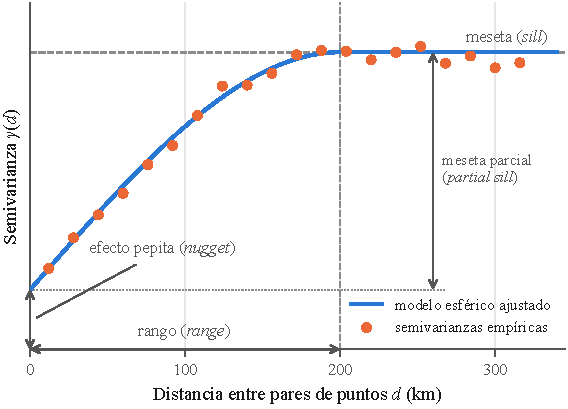
\includegraphics[width=0.66\textwidth]{fig_semivariograma}}{\fbox{figura pendiente}}
  \caption{Semivariograma esquemático: semivarianzas empíricas por clase de
  distancia y modelo esférico ajustado, con sus tres parámetros: efecto
  pepita (valor en el origen), meseta (valor estable) y rango (distancia a
  la que se alcanza la meseta), que aquí fija el tamaño de los bloques de
  validación.}
  \label{fig:semivariograma}
\end{figure}
 Si entrenamiento y prueba se reparten al azar, cada punto de
prueba tiene vecinos casi idénticos en entrenamiento y las métricas resultan
infladas \citep[pp.~276, 297]{guisan2017hsdm}. En audio el consejo es el
mismo: nunca repartir grabaciones de un mismo lugar o archivo entre
entrenamiento y prueba \citep[pp.~161, 166]{virtanen2018casse}. La
validación cruzada por bloques \citep{roberts2017crossvalidation,
valavi2019blockcv} divide el territorio en bloques contiguos de tamaño
comparable al rango de autocorrelación, asigna los bloques al azar a cinco
\textit{folds} y evalúa cada modelo en bloques que nunca vio. Mide, por
tanto, la capacidad de
\emph{extrapolar} a zonas sin registros, que es más exigente que la de
interpolar entre registros vecinos (\figref{fig:blockcv}). Ambos protocolos
se reportan en el \capref{cap:resultados}.


%-----------------------------------------------------------------------
\section{Metodología de trabajo, fuentes de datos y \textit{baselines}}
\label{sec:herramientas}

\subsection{Metodología de trabajo}

El proyecto se organiza según la metodología CRISP-DM: comprensión del
problema, comprensión y preparación de los datos (\capref{cap:datos}),
modelado, evaluación y despliegue (\capref{cap:resultados}), fases recorridas de
forma iterativa. Todo el desarrollo se realiza en Python con PyTorch
\citep{paszke2019pytorch}, sobre
un repositorio versionado cuyas dependencias se gestionan con \texttt{uv}
para garantizar la reproducibilidad de los experimentos.

\subsection{Fuentes de datos}

La \tabref{tab:fuentes} resume las fuentes públicas integradas, su
modalidad, cobertura y uso en el proyecto. MODIS es el sensor de los
satélites Terra y Aqua de la NASA del que proviene el NDVI. Google Earth
Engine (GEE) no es una fuente de datos, sino la plataforma en la nube desde
la que se consultan MODIS, WorldClim y SRTM sin descargar las imágenes
completas (\secref{sec:covariables}).

\begin{table}[!htb]
  \centering\footnotesize
  \caption{Fuentes de datos integradas en el proyecto. El plan original
  contemplaba ERA5 \citep{hersbach2020era5} y Sentinel-2
  \citep{drusch2012sentinel2}; su reemplazo se explica en el
  \capref{cap:datos}.}
  \label{tab:fuentes}
  \begin{tabularx}{\textwidth}{@{}>{\raggedright\arraybackslash\hsize=1.2\hsize}X l l l >{\raggedright\arraybackslash\hsize=0.8\hsize}X@{}}
    \toprule
    Fuente & Modalidad & Cobertura & Licencia & Uso en el proyecto \\
    \midrule
    Xeno-canto \citep{vellinga2015xenocanto} & Audio & Global & CC (varias) & Grabaciones etiquetadas por especie focal \\
    iNaturalist / GBIF \citep{vanhorn2018inaturalist} & Imagen & Global & CC (varias) & Fotografías geolocalizadas con grado de investigación \\
    eBird e iNaturalist vía GBIF \citep{sullivan2014ebird} & Tabular & Global & Abierta (CC) & Registros de presencia georreferenciados con fecha \\
    MODIS vía GEE \citep{didan2021mod13a2, gorelick2017gee} & Satelital & Global, \SI{1}{\kilo\metre} & Abierta & NDVI por punto y año \\
    WorldClim y SRTM vía GEE \citep{hijmans2005worldclim, farr2007srtm} & Climática, topográfica & Global, \SI{1}{\kilo\metre} & Abierta & Temperatura, precipitación y elevación \\
    RCE -- MMA \citep{mma2026rce} & Documental & Chile & Pública & Categoría de conservación; selección de especies \\
    \bottomrule
  \end{tabularx}
\end{table}

\subsection{Selección de \textit{baselines}}

Los \textit{baselines} se eligieron pensando en dos dimensiones: cómo se
abordaría cada problema \emph{hoy, sin este proyecto}, y cómo se abordaría
\emph{con un método más antiguo o más simple}. La \tabref{tab:baselines-def}
los organiza por tarea y resume la configuración de cada uno. Los
hiperparámetros completos están en el Apéndice~\ref{ape:hiperparametros}.

\begin{table}[!htb]
  \centering\footnotesize
  \caption{\textit{Baselines} del proyecto, por tarea y por dimensión de
  comparación.}
  \label{tab:baselines-def}
  \begin{tabularx}{\textwidth}{@{}>{\raggedright\arraybackslash\hsize=0.55\hsize}X >{\raggedright\arraybackslash\hsize=1.25\hsize}X >{\raggedright\arraybackslash\hsize=1.2\hsize}X@{}}
    \toprule
    Tarea & Práctica actual (sin este proyecto) & Método más simple o más antiguo \\
    \midrule
    Identificación de especies &
    (i) Clasificadores unimodales (solo audio o solo imagen), la forma
    habitual de identificación automática: los mismos modelos de esta tesis
    evaluados sin fusión.
    (ii) Un modelo de IA generativa multimodal (Claude Opus 5.5) consultado
    con la fotografía y la lista de especies candidatas, en
    \textit{zero-shot} y \textit{few-shot} (una fotografía de referencia por
    especie); temperatura por defecto (1,0), esfuerzo de razonamiento bajo,
    salida estructurada restringida a la lista. &
    Regresión logística sobre los \textit{frozen embeddings} de los mismos
    modelos preentrenados sin ajustar (EfficientNet-B0 y B3 de ImageNet,
    AST de AudioSet), siguiendo a \citet{ghani2023embeddings}: mide cuánto
    aporta el ajuste completo. \\
    \midrule
    Distribución de especies &
    MaxEnt, el método de referencia en ecología, implementado como regresión
    logística penalizada (L2, $C = 1$) con \textit{features} lineales y
    cuadráticas (Ecuación~\ref{eq:logistica}). &
    El propio MaxEnt es también el método clásico; frente a él se comparan
    Random Forest ($B = 300$), gradient boosting ($J = 300$, $\nu = 0{,}05$)
    y la red neuronal conjunta (Ecuación~\ref{eq:deepsdm}). \\
    \bottomrule
  \end{tabularx}
\end{table}

%-----------------------------------------------------------------------
\section{Justificación técnica de la metodología}\label{sec:justificacion}

\textbf{Transfer learning.} El conjunto de datos chileno es pequeño
(\num{2508} grabaciones de 55 especies y \num{7060} fotografías de 53), lo que
hace inviable entrenar redes profundas desde cero. Los modelos preentrenados
en ImageNet y AudioSet reutilizan representaciones aprendidas sobre millones
de ejemplos y solo necesitan ajustarse a la nueva tarea
(\secref{sec:teoria-transfer}). Que los \textit{embeddings} de clasificadores
de aves transfieran incluso con pocos ejemplos por clase
\citep{ghani2023embeddings} es valioso para las especies amenazadas, que son
las que menos datos tienen.

\textbf{Late fusion.} Aporta robustez frente a registros ambiguos o
incompletos: un canto grabado con ruido puede complementarse con una
fotografía y viceversa. Permite entrenar cada rama con datos no
emparejados, que es la situación de Xeno-canto e iNaturalist, donde audio e
imagen de un mismo individuo raramente coexisten, y opera cuando solo hay
una modalidad (\secref{sec:teoria-fusion}). Los resultados de SSW60
muestran que esta combinación mejora el desempeño sobre cada modalidad por
separado \citep{vanhorn2022ssw60}.

\textbf{Balanceo y aumentación.} La pérdida ponderada por clase, SpecAugment
y \textit{mixup} (\secref{sec:teoria-regularizacion}) abordan el desbalance
y la escasez propios de los datos de ciencia ciudadana. Sin ellas, el
clasificador se sesgaría hacia las especies comunes en desmedro de las
amenazadas y memorizaría un corpus de pocas decenas de grabaciones por
especie.

\textbf{Covariables ambientales.} Google Earth Engine muestrea las
covariables en la nube sobre todo el territorio continental y evita
descargar y almacenar volúmenes masivos de imágenes satelitales
\citep{gorelick2017gee}. Las climatologías grilladas de WorldClim son el
conjunto de datos climáticos más usado en ecología y ofrecen cobertura
nacional homogénea, más práctica a escala que las estaciones
meteorológicas, cuya distribución en Chile es irregular
\citep[p.~63]{guisan2017hsdm}.

\textbf{Modelado de distribución.} La red conjunta multiespecie comparte
información estadística entre especies con distribuciones similares, lo que
beneficia a las de pocos registros. Los ensambles de árboles aportan una
referencia fuerte y robusta en datos tabulares
\citep{valavi2022benchmark}, y MaxEnt, como regresión logística, aporta
interpretabilidad. La validación espacial por bloques
(\secref{sec:teoria-validacion}) permite comprobar que la comparación no
esté inflada por autocorrelación.

\textbf{Baselines exigentes.} Elegir MaxEnt, un modelo de IA generativa y
los \textit{frozen embeddings} como referencias asegura que las mejoras
reportadas sean significativas en la práctica y no artefactos de una
comparación débil.

%-----------------------------------------------------------------------
\section{Efectos positivos esperados}\label{sec:efectos}

Se espera que el sistema identifique al menos 50 especies de aves chilenas
con una \textit{accuracy} superior al \SI{85}{\percent}, que la fusión
multimodal supere a los clasificadores unimodales en \textit{accuracy} y F1
macro y que el SDM basado en aprendizaje automático supere a MaxEnt en
AUC-ROC. Más allá de las métricas, los efectos positivos esperados de la
aplicación de estos elementos son:

\begin{enumerate}[label=(\roman*), leftmargin=*, itemsep=2pt]
  \item Una herramienta de apoyo al monitoreo automatizado de biodiversidad
        para organismos de conservación (MMA, CONAF, SAG) y ONG (ROC,
        CODEFF), alineada con las líneas de acción de investigación y
        monitoreo de la Estrategia Nacional de Conservación de Aves
        \citep{mma2022enca}.
  \item Un insumo para la ciencia ciudadana y la identificación asistida de
        aves, que puede retroalimentar la calidad de los registros en
        plataformas como eBird e iNaturalist.
  \item Mapas de probabilidad de presencia que permitan priorizar zonas de
        monitoreo y evaluar el efecto de variables climáticas y de vegetación
        sobre la distribución de especies amenazadas.
  \item Un repositorio reproducible que reduzca el costo de entrada para
        futuros trabajos sobre otras especies o regiones.
  \item Evidencia metodológica cuantitativa sobre la escasez de datos en
        especies amenazadas y sobre la efectividad de las estrategias de
        mitigación, útil para orientar esfuerzos de recolección de datos.
\end{enumerate}


\chapter{Levantamiento de datos}\label{cap:datos}
%=======================================================================
% cap4_datos.tex — Levantamiento de datos
%=======================================================================

Este capítulo documenta las fases de comprensión y preparación de los datos:
cómo se definió el conjunto de especies, cómo se construyeron los tres corpus
del sistema (audio, imagen y avistamientos con covariables ambientales), qué
decisiones se tomaron durante el levantamiento y en qué se apartó la
implementación del plan original.

%-----------------------------------------------------------------------
\section{Repositorio reproducible y acceso a las fuentes}\label{sec:repositorio}

El levantamiento se implementó como una secuencia de \textit{scripts}
numerados sobre un paquete Python (\texttt{biomonitor}) con módulos de
datos, audio, visión, fusión multimodal y distribución de especies. Las
dependencias se fijan con \texttt{uv} y Python 3.12, los hiperparámetros
viven en un único archivo de configuración y las credenciales se cargan
desde variables de entorno. Las descargas y los entrenamientos se ejecutaron
en un Mac con procesador Apple M4 Pro, con aceleración por GPU mediante
Metal/MPS. El código, la configuración y los \textit{scripts} están
publicados en \url{\repoURL}.

Las fuentes se consultan mediante sus interfaces programáticas: la API v3 de
Xeno-canto, la API pública de GBIF para fotografías y registros de
ocurrencia, y Google Earth Engine (GEE) para las covariables ambientales. El
listado del RCE se descarga directamente del sitio del Ministerio del Medio
Ambiente. Los modelos preentrenados provienen de los repositorios abiertos
\texttt{timm} y Hugging Face.

%-----------------------------------------------------------------------
\section{Conjunto de especies objetivo}\label{sec:especies}

El conjunto objetivo se construyó a partir del listado oficial del
Reglamento de Clasificación de Especies (RCE), que asigna a cada especie
evaluada una categoría de conservación. La \tabref{tab:rce} resume las
categorías que aparecen en este trabajo y la \figref{fig:seleccion} muestra
el proceso de selección completo.

\begin{table}[!htb]
  \centering\small
  \caption{Categorías de conservación del RCE que aparecen en este trabajo y
  número de especies del conjunto objetivo en cada una.}
  \label{tab:rce}
  \begin{tabular}{@{}l l l r@{}}
    \toprule
    Sigla & Categoría & Significado & Especies \\
    \midrule
    CR & En Peligro Crítico & riesgo extremadamente alto de extinción & 1 \\
    EN & En Peligro & riesgo muy alto de extinción & 5 \\
    VU & Vulnerable & riesgo alto de extinción & 7 \\
    NT & Casi Amenazada & cerca de calificar como amenazada & 1 \\
    LC & Preocupación Menor & evaluada y sin riesgo actual & 3 \\
    NE & No Evaluada & sin evaluación formal en el RCE & 38 \\
    \bottomrule
  \end{tabular}
\end{table}

\begin{figure}[!htb]
  \centering
  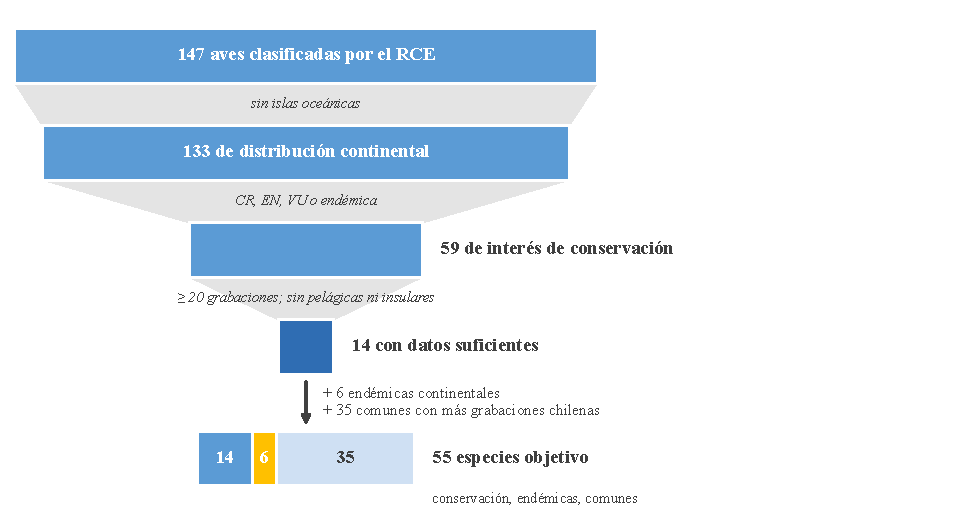
\includegraphics[width=\textwidth]{fig_seleccion_especies}
  \caption{Construcción del conjunto de 55 especies objetivo: de las 147
  aves clasificadas por el RCE se conservan las de distribución continental,
  luego las de interés de conservación y por último las que tienen datos
  suficientes; a esas 14 se suman 6 endémicas y 35 comunes.}
  \label{fig:seleccion}
\end{figure}

El punto de partida son las 147 aves clasificadas por el RCE. Primero se
filtraron las de distribución continental (133) y, entre ellas, las de
interés de conservación (CR, EN o VU, o endémicas de Chile), lo que dejó 59
candidatas. Para cada una se realizó un censo de datos: grabaciones en
Xeno-canto (globales y con localidad en Chile) y fotografías con grado de
investigación en GBIF. Se descartaron las especies pelágicas (aves marinas
que viven en mar abierto, como albatros, petreles y pingüinos) e insulares
(restringidas a las islas oceánicas), cuyo monitoreo responde a otra lógica,
y las que no alcanzaban un mínimo de 20 grabaciones a nivel global. Quedaron
14 especies de interés de conservación: una CR (\textit{Podiceps
gallardoi}), cinco EN, siete VU y el choroy (\textit{Enicognathus
leptorhynchus}), endémico en Preocupación Menor. Segundo, se agregaron las
seis especies endémicas continentales restantes con grabaciones suficientes
(tenca, chiricoca, turca, hued-hued castaño, tapaculo y churrín del norte).
Tercero, se completó el conjunto con las 35 especies comunes con mayor
número de grabaciones chilenas en Xeno-canto, que aportan masa de
entrenamiento y representan los principales ecosistemas del país. En el
resto del documento las especies se agrupan en tres categorías:
\emph{amenazadas} (13 especies CR, EN o VU), \emph{endémicas} no amenazadas
(7, incluido el choroy) y \emph{comunes} (35). El listado completo se
presenta en el Apéndice~\ref{ape:especies}.


La exclusión de las pelágicas no es solo una decisión de datos. Cerca de 25
de las 59 candidatas lo son, apenas vocalizan en tierra y su distribución es
oceánica, incompatible con un modelo de distribución terrestre basado en
vegetación y clima. La consecuencia es que no es posible reunir 50 especies
únicamente con aves amenazadas, lo que obligó a completar el conjunto con
especies comunes. La propuesta original pedía ``foco'' en las amenazadas, no
exclusividad, y esa composición preserva el foco con una base de
entrenamiento suficiente.

%-----------------------------------------------------------------------
\section{Corpus de audio}\label{sec:corpus-audio}

\subsection{Censo y disponibilidad}

El censo identificó \num{2587} grabaciones de Xeno-canto con localidad en
Chile para las 55 especies. La \tabref{tab:corpus-grupos} resume la
disponibilidad por grupo y la \figref{fig:corpus} la detalla por especie. La
asimetría es fuerte. Las 13 especies amenazadas reúnen 129 grabaciones
chilenas, el \SI{5}{\percent} del total, con una mediana de 6 por especie, y
cuatro de ellas no tienen ninguna. Las 35 comunes concentran el
\SI{81}{\percent}. La especie más grabada (\textit{Turdus falcklandii}, 186)
tiene por sí sola más audio que las 13 amenazadas juntas.

\begin{table}[!htb]
  \centering\small
  \caption{Grabaciones de Xeno-canto con localidad en Chile por grupo de
  especies del conjunto objetivo.}
  \label{tab:corpus-grupos}
  \fitwidth{\begin{tabular}{@{}l r r r r r r@{}}
    \toprule
    Grupo & Especies & Grabaciones & \% del total & Mínimo & Mediana & Máximo \\
    \midrule
    Amenazadas (CR, EN, VU) & 13 & 129 & 5,0 & 0 & 6 & 34 \\
    Endémicas (incl.\ choroy) & 7 & 355 & 13,7 & 34 & 46 & 86 \\
    Comunes & 35 & \num{2103} & 81,3 & 32 & 51 & 186 \\
    \midrule
    Total & 55 & \num{2587} & 100 & 0 & 44 & 186 \\
    \bottomrule
  \end{tabular}}
\end{table}

\begin{figure}[!htb]
  \centering
  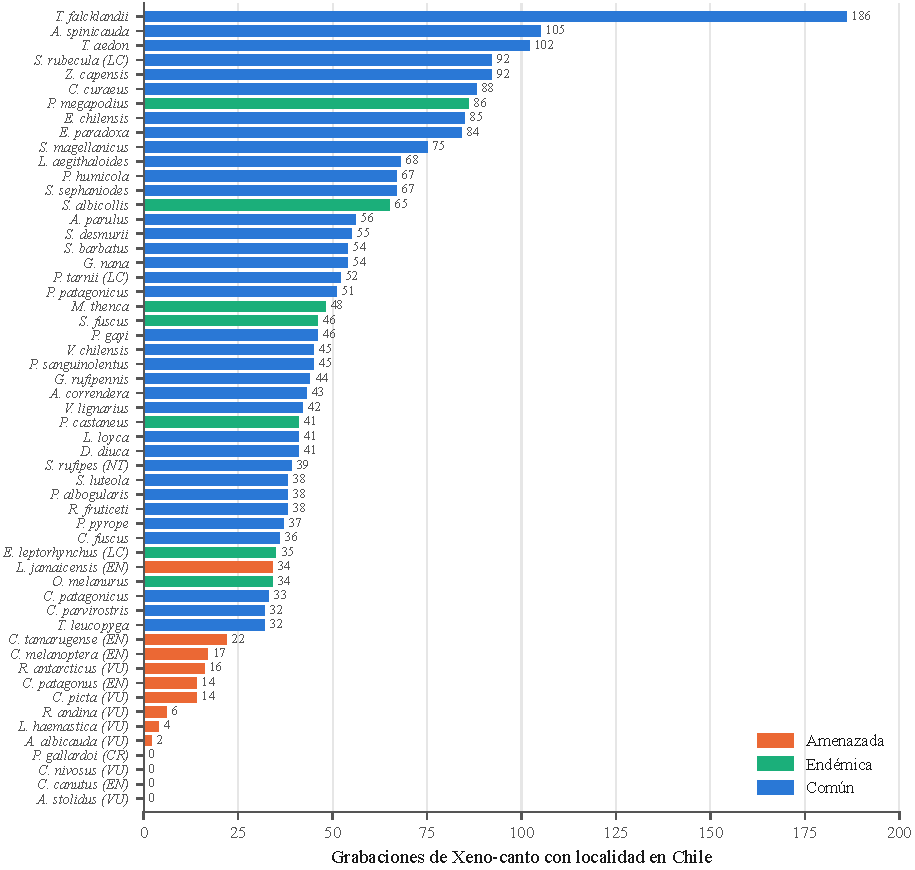
\includegraphics[width=0.95\textwidth]{fig_corpus_especies}
  \caption{Grabaciones de Xeno-canto con localidad en Chile por especie del
  conjunto objetivo, coloreadas por grupo. Entre paréntesis, la categoría del
  RCE cuando la especie ha sido evaluada.}
  \label{fig:corpus}
\end{figure}

\subsection{Descarga y composición del corpus}

Dado el censo anterior, el corpus de entrenamiento no se limitó a Chile. Para
cada especie se descargaron hasta 50 grabaciones de calidad A, B o C y de
menos de cuatro minutos, priorizando las de localidad chilena y completando
con grabaciones de otros países cuando faltaban. La calidad es la que asignan
los propios usuarios de Xeno-canto en una escala de A (grabación nítida, con
el ave en primer plano y casi sin ruido) a E (apenas audible). Se conservaron
las tres mejores. Dos razones justifican el uso de audio extranjero. La
primera es acústica: la firma vocal es específica de la especie y, para aves
de distribución amplia, las poblaciones vecinas comparten el repertorio. La
segunda es práctica: sin grabaciones externas, las cuatro especies
amenazadas sin audio chileno quedarían fuera del clasificador. El tope de 50
por especie acota el desbalance, pues las comunes tendrían hasta 186. La
\tabref{tab:corpus-audio} resume el corpus resultante y la
\figref{fig:datos-especie} muestra su composición por especie y origen.

\begin{figure}[p]
  \centering
  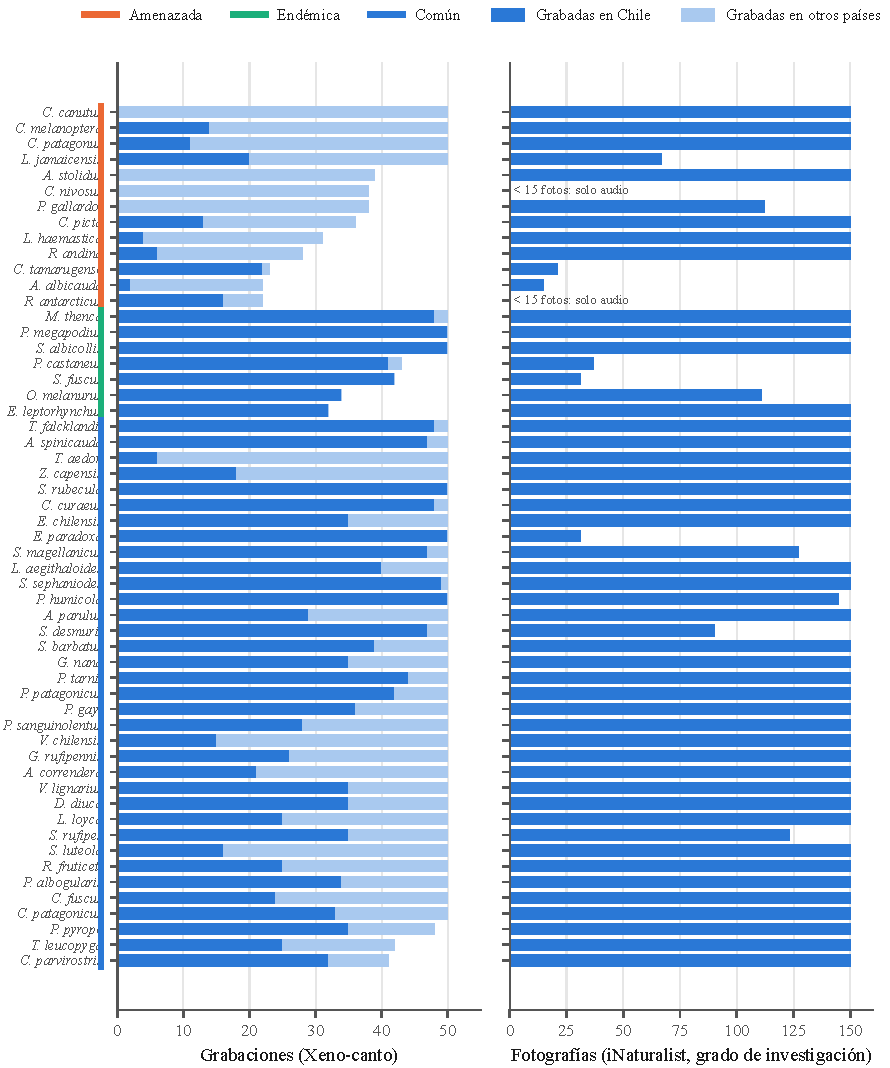
\includegraphics[width=0.88\textwidth]{fig_datos_por_especie}
  \caption{Composición de los corpus por especie; las especies se ordenan por grupo
  de conservación (franja de color) y número de grabaciones. Izquierda:
  grabaciones de audio del corpus de entrenamiento según su origen.
  Derecha: fotografías con grado de investigación de iNaturalist. Las dos
  especies con menos de 15 fotografías no participan del clasificador de
  imagen.}
  \label{fig:datos-especie}
\end{figure}

\begin{table}[!htb]
  \centering\small
  \caption{Corpus de audio descargado y preprocesado.}
  \label{tab:corpus-audio}
  \begin{tabularx}{\textwidth}{@{}l X@{}}
    \toprule
    Característica & Valor \\
    \midrule
    Grabaciones & \num{2509} seleccionadas; \num{2508} decodificadas correctamente (una corrupta) \\
    Duración total & \SI{25,6}{\hour} (mediana \SI{24}{\second} por grabación; \SI{7}{\percent} dura \SI{5}{\second} o menos) \\
    Grabaciones por especie & mínimo 22 (\textit{Agriornis albicauda}, \textit{Rallus antarcticus}), tope 50; 39 especies alcanzan el tope \\
    Origen & \SI{64}{\percent} Chile (\num{1609}); \SI{36}{\percent} de otros 36 países (Argentina 434, Brasil 77, Ecuador 56, Perú 45, Estados Unidos 44) \\
    Especies con menos de la mitad de audio chileno & 17; cuatro sin ninguna grabación chilena (\textit{P.~gallardoi}, \textit{C.~canutus}, \textit{C.~nivosus}, \textit{A.~stolidus}) \\
    Calidad de la grabación (escala de Xeno-canto) & A \SI{69}{\percent}, B \SI{26}{\percent}, C \SI{4}{\percent} \\
    Tipo de vocalización & canto en el \SI{47}{\percent} de las grabaciones, llamado en el \SI{56}{\percent} (categorías no excluyentes) \\
    Particiones (grabaciones) & entrenamiento \num{1721} (\SI{69}{\percent}), validación 394 (\SI{16}{\percent}), prueba 393 (\SI{16}{\percent}) \\
    \bottomrule
  \end{tabularx}
\end{table}

\subsection{Preprocesamiento y particiones}

Cada archivo se decodificó, se convirtió a mono, se remuestreó a
\SI{32}{\kilo\hertz} y se almacenó en una caché comprimida sin pérdida
junto a un manifiesto con sus metadatos (especie, identificador de
Xeno-canto, duración, país, calidad y tipo de vocalización). Las particiones
de entrenamiento, validación y prueba (70/15/15) se construyeron a nivel de
\emph{grabación}, estratificadas por especie y con semilla fija, de modo que
todas las ventanas extraídas de un mismo archivo pertenecen a una única
partición. Las 55 especies están presentes en las tres
particiones. El conjunto de prueba tiene entre 3 (\textit{A.~albicauda}) y 8
grabaciones por especie, lo que, como se verá en el
\capref{cap:resultados}, hace ruidosas las métricas de las especies raras.

%-----------------------------------------------------------------------
\section{Corpus de imagen}\label{sec:corpus-imagen}

Las fotografías provienen de observaciones de iNaturalist con grado de
investigación, es decir, geolocalizadas y con la identificación validada por
la comunidad. Se descargaron a través de la API de GBIF \citep{inat2026gbif}
con un tope de 150 por especie. La descarga exigió dos ajustes. Primero, un
mapa de sinónimos taxonómicos: iNaturalist clasifica al fío-fío como
\textit{Elaenia albiceps} y escribe \textit{Sylviorthorhynchus desmursii}
para el colilarga, por lo que las consultas con los nombres del RCE
devolvían cero resultados. Segundo, un respaldo filtrado para las especies
con pocas fotografías: al ampliar la búsqueda a todo GBIF aparecían
espectrogramas de Xeno-canto y fotografías de especímenes de museo, de modo
que se restringió a observaciones humanas de aves vivas.

Se obtuvieron \num{7068} fotografías para las 55 especies. Dos especies
amenazadas no alcanzaron el mínimo de 15 fotografías de aves vivas
(\textit{Charadrius nivosus}, con 2, y \textit{Rallus antarcticus}, con 6)
y quedaron fuera del clasificador de imagen como especies \emph{solo audio},
que la fusión multimodal sigue cubriendo. El corpus del clasificador tiene,
por tanto, \num{7060} fotografías de 53 especies, entre 15
(\textit{A.~albicauda}) y 150 por especie, con solo dos especies bajo 30. El
\SI{52}{\percent} de las fotografías fue tomado en Chile y el
\SI{33}{\percent} en Argentina. Como cada fotografía es una observación
independiente, la partición se hizo a nivel de fotografía, estratificada por
especie y con la misma semilla: \num{4980} para entrenamiento, \num{1040}
para validación y \num{1040} para prueba. El mismo patrón de escasez del
audio reaparece aquí: las especies de mayor interés de conservación son las
que tienen menos ejemplos y conjuntos de prueba de 2 a 5 fotografías.

%-----------------------------------------------------------------------
\section{Avistamientos y covariables ambientales}\label{sec:datos-sdm}

\subsection{Registros de presencia}

Los registros de presencia para el modelo de distribución se obtuvieron de la
búsqueda pública de ocurrencias de GBIF, que agrega las observaciones de
eBird \citep{ebird2026gbif} e iNaturalist, con un tope de \num{2000} registros
por especie dentro de Chile continental (coordenadas válidas y dentro del
rectángulo de latitud \SIrange{-56}{-17,5}{\degree} y longitud
\SIrange{-75,7}{-66,4}{\degree}, que excluye las islas oceánicas). El plan
original contemplaba la base histórica de eBird (EBD), que entrega listas
completas con el esfuerzo de observación. La solicitud de acceso se envió en
julio de 2026 y, al momento de escribir este informe (octubre de 2026), no
ha sido aprobada, de modo que se optó por GBIF, que es inmediato y
reproducible. El costo de esta decisión es la pérdida del esfuerzo de
observación, que se compensa en la generación de pseudoausencias
(\secref{sec:pseudoausencias}).

Se reunieron \num{100270} registros de las 55 especies. Cuarenta y nueve
especies alcanzan el tope y cinco quedan por debajo de 500 (\textit{Anous
stolidus} tiene solo 5 y no se modela). La \figref{fig:avistamientos}
muestra su distribución. Espacialmente, siguen la geografía del esfuerzo de
observación, concentrados en la zona central y en torno a las ciudades y
rutas, y el patrón apenas cambia entre verano e invierno. Temporalmente, el
\SI{87}{\percent} corresponde a 2024--2026, por el crecimiento reciente de la
ciencia ciudadana y porque el tope por especie favorece los registros más
recientes. Estacionalmente, la mitad (\SI{51}{\percent}) se concentra en enero
y febrero, el verano austral. Esta estacionalidad mezcla la fenología de
las aves con el esfuerzo de los observadores y es una de las limitaciones
que se discuten en el \capref{cap:conclusiones}.

\begin{figure}[!htb]
  \centering
  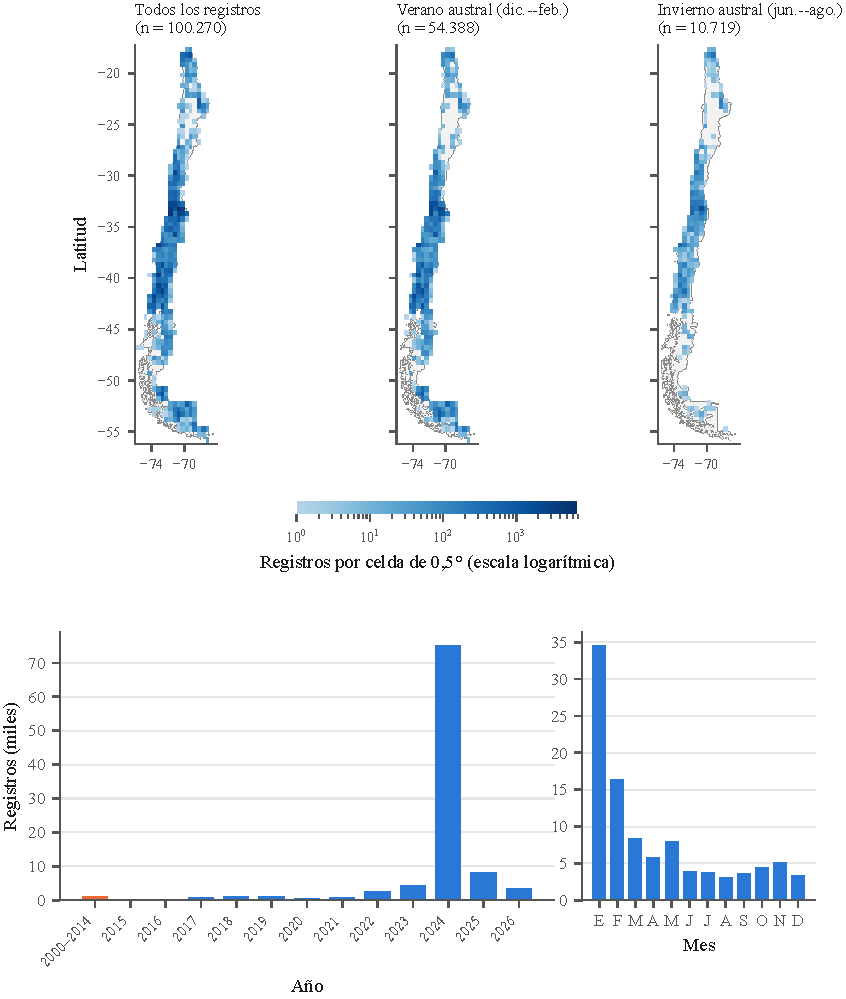
\includegraphics[width=0.92\textwidth]{fig_avistamientos}
  \caption{Registros de presencia obtenidos de GBIF (eBird e iNaturalist) para
  las 55 especies. Arriba: densidad espacial en celdas de \SI{0,5}{\degree}
  para todos los registros, para el verano y para el invierno austral.
  Abajo: distribución por año y por mes.}
  \label{fig:avistamientos}
\end{figure}

\subsection{Pseudoausencias y conjunto de datos del SDM}\label{sec:pseudoausencias}

Un modelo de distribución necesita contrastar los lugares donde la especie
está con lugares donde no está. Los registros de ciencia ciudadana solo
dicen dónde se la vio, nunca dónde se la buscó sin éxito, así que las
``ausencias'' deben construirse artificialmente: son las
\emph{pseudoausencias} o puntos de fondo (\secref{sec:teoria-sdm}). La
forma más simple, repartirlas al azar por todo el territorio, tiene un
problema: los avistamientos se concentran donde hay observadores, de modo
que el modelo aprendería a distinguir ``lugares con gente'' de ``lugares sin
gente'' en vez de hábitat bueno y malo. Para evitarlo se usó el método del
\emph{grupo objetivo} \citep{phillips2009bias}: se tomó una única muestra
aleatoria de \num{10000} avistamientos de todas las especies del conjunto,
compartida entre todas las especies modeladas, que por construcción
reproduce los lugares y meses en que la gente observa aves; cada modelo usa
\num{1500} de esos puntos como fondo (Apéndice~\ref{ape:hiperparametros}).
Así, el contraste que aprende el modelo es entre los sitios donde se vio a
la especie y los sitios comparables donde se observan aves en general. Las
presencias se limitaron a 500 registros por especie para reducir el peso de
las zonas sobremuestreadas. Tras muestrear las covariables, el conjunto de
datos quedó en \num{34926} puntos: \num{25171} presencias de 55 especies (54
con al menos 20, el mínimo para modelar) y \num{9755} puntos de fondo (los
245 restantes cayeron sobre agua o sin datos).

\subsection{Covariables ambientales}\label{sec:covariables}

Cada punto (presencia o pseudoausencia) se describe con cuatro variables
ambientales y el mes del registro (\tabref{tab:covariables},
\figref{fig:covariables}). Las variables ambientales se obtuvieron de
Google Earth Engine, una plataforma de Google que almacena en la nube
catálogos de imágenes satelitales y capas climáticas y permite consultarlos
sin descargarlos \citep{gorelick2017gee}. Para cada punto se pidió, en una
sola consulta, el valor de las cuatro capas a \SI{1}{\kilo\metre} de
resolución. El NDVI (índice de vegetación de diferencia normalizada) mide la
cantidad de vegetación verde a partir de la luz que refleja la superficie y
proviene de MODIS, un sensor de los satélites Terra y Aqua de la NASA que
observa toda la Tierra cada uno o dos días. La temperatura media anual y la
precipitación anual provienen de WorldClim, una climatología global
interpolada a partir de estaciones meteorológicas. La elevación proviene del
modelo digital de terreno SRTM. El mes del avistamiento se codifica de forma
cíclica (seno y coseno), lo que aporta el eje temporal al modelo.

\begin{figure}[!htb]
  \centering
  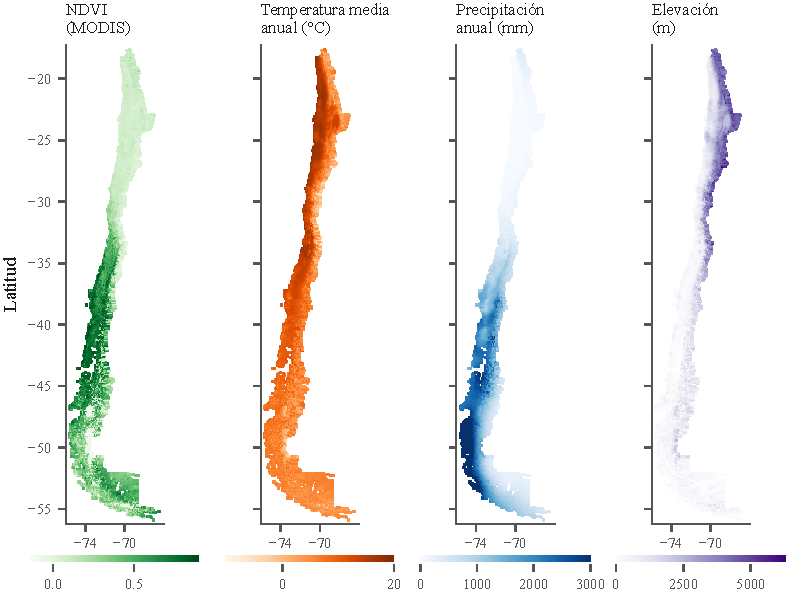
\includegraphics[width=0.9\textwidth]{fig_covariables}
  \caption{Covariables ambientales sobre la grilla de \SI{0,1}{\degree} de
  Chile continental: NDVI, temperatura media anual, precipitación anual
  (escala truncada en \SI{3000}{\milli\metre}) y elevación.}
  \label{fig:covariables}
\end{figure}

El plan original usaba el reanálisis climático ERA5 y el NDVI mensual de
Sentinel-2. Ambos se descartaron por una restricción de cómputo de la
plataforma: calcular la mediana de miles de imágenes de Sentinel-2 o el
promedio de 120 meses de ERA5 en decenas de miles de puntos excede el tiempo
máximo que Google Earth Engine permite por consulta. Se reemplazaron por
capas precalculadas, que son además el estándar en modelado de distribución
\citep{hijmans2005worldclim}. Para los experimentos con información satelital
se extrajeron también parches de cobertura de suelo de ESA WorldCover
\citep{zanaga2021worldcover} y el \textit{embedding} satelital anual de 64
dimensiones de Google (AlphaEarth Foundations, \citealp{brown2025alphaearth}).
Este \textit{embedding} es una representación numérica de cada píxel,
aprendida por un modelo de fundación a partir de múltiples satélites, y se
usó en su versión fija (2023) y pareada al año de cada observación
(2017--2025). Para dibujar mapas de
distribución se muestrearon las mismas covariables en una grilla regular de
\SI{0,1}{\degree} (\num{7910} celdas dentro de Chile continental).

\begin{table}[!htb]
  \centering\small
  \caption{Covariables del modelo de distribución.}
  \label{tab:covariables}
  \begin{tabularx}{\textwidth}{@{}l l l X@{}}
    \toprule
    Covariable & Fuente & Resolución & Rango en el conjunto de datos \\
    \midrule
    NDVI (media anual 2022) & MODIS MOD13A2 \citep{didan2021mod13a2} & \SI{1}{\kilo\metre} & $-0{,}15$ a $0{,}89$ \\
    Temperatura media anual & WorldClim v1 (bio01) & \SI{1}{\kilo\metre} & $-1{,}4$ a \SI{19,9}{\celsius} \\
    Precipitación anual & WorldClim v1 (bio12) & \SI{1}{\kilo\metre} & 0 a \SI{3866}{\milli\metre} \\
    Elevación & SRTM \citep{farr2007srtm} & \SI{30}{\metre} & $-1$ a \SI{5104}{\metre} \\
    Mes (seno, coseno) & fecha del registro & -- & ciclo anual \\
    \bottomrule
  \end{tabularx}
\end{table}


%-----------------------------------------------------------------------
\section{Hallazgos del levantamiento y desviaciones del plan}\label{sec:hallazgos}

\subsection{Escasez de datos en las especies amenazadas}

El hallazgo transversal del levantamiento es la asimetría de datos entre
categorías de conservación. En audio, las 13 especies amenazadas reúnen el
\SI{5}{\percent} de las grabaciones chilenas (\tabref{tab:corpus-grupos}). En
imagen, las dos únicas especies excluidas del clasificador por falta de
fotografías son amenazadas, y las de menor conjunto de prueba también lo
son. En avistamientos, las cinco especies con menos de 500 registros son
amenazadas. Este patrón refleja un sesgo estructural de la ciencia
ciudadana: se registra más lo que es más fácil de encontrar. Su implicancia
es que un sistema de monitoreo orientado a conservación no puede diseñarse
asumiendo abundancia de datos para las especies que más importa detectar. El
censo aporta también la vía de mitigación: varias amenazadas de distribución
amplia tienen mucho más audio fuera del país (\textit{Calidris canutus} tiene
311 grabaciones globales y \textit{Laterallus jamaicensis}, 181), lo que permitió
entrenar con grabaciones de otras poblaciones y medir después el efecto del
origen de la grabación (\secref{sec:res-audio}).

\subsection{Desviaciones respecto del plan}

La \tabref{tab:desviaciones} resume las diferencias entre la propuesta
(Capítulos~\ref{cap:intro} a \ref{cap:teoria}) y lo implementado, con su
motivo. Corresponden a los riesgos del proyecto que se materializaron, todos
detectados durante el levantamiento: acceso a datos restringidos, cómputo
insuficiente y datos de menor calidad que la prevista. Ninguna altera las
preguntas de investigación, y sus consecuencias se discuten en el
\capref{cap:conclusiones}.

\begin{table}[!htb]
  \centering\footnotesize
  \caption{Desviaciones entre lo planificado y lo implementado.}
  \label{tab:desviaciones}
  \begin{tabularx}{\textwidth}{@{}>{\raggedright\arraybackslash\hsize=0.7\hsize}X
    >{\raggedright\arraybackslash\hsize=1.0\hsize}X
    >{\raggedright\arraybackslash\hsize=1.3\hsize}X@{}}
    \toprule
    Planificado & Implementado & Motivo y consecuencia \\
    \midrule
    Avistamientos de eBird (EBD) con esfuerzo y listas completas & Ocurrencias de GBIF (eBird + iNaturalist), sin esfuerzo & La EBD, solicitada en julio, no fue aprobada a tiempo. Sin esfuerzo, el sesgo de muestreo se corrige con fondo de grupo objetivo. \\
    \midrule
    Clima ERA5 (Copernicus) & WorldClim v1 (bio01, bio12) & El muestreo de ERA5 en \num{35000} puntos excede el cómputo de GEE. WorldClim es el estándar en SDM. \\
    \midrule
    NDVI mensual de Sentinel-2 (\SI{10}{\metre}) & NDVI anual de MODIS (\SI{1}{\kilo\metre}) y \textit{embeddings} satelitales anuales & Idéntica restricción de cómputo. La dimensión temporal se evaluó con el pareo anual del satélite. \\
    \midrule
    EfficientNet y ViT a resolución completa (ConvNeXt o ViT-B preentrenados en ImageNet-21k, \SI{384}{px}) & EfficientNet-B3 a \SI{384}{px} (ImageNet y NoisyStudent) y ViT-S/16 a \SI{224}{px} & Un ConvNeXt preentrenado en ImageNet-21k tardaba unas 8 horas por época en el equipo disponible y se descartó; ViT-B a \SI{384}{px} resultó inviable por el mismo motivo. La variante pequeña ViT-S/16 sí se entrenó y quedó entre seis y ocho puntos por debajo de B3 según el protocolo (\secref{sec:res-imagen}). \\
    \midrule
    Pérdida balanceada por número efectivo de muestras & Pesos inversos a la frecuencia ($\beta \to 1$) con suavizado de etiquetas y \textit{mixup} & Caso límite de la misma familia. El desbalance del corpus es moderado (22 a 50 grabaciones). \\
    \midrule
    Evaluación de audio solo sobre grabaciones chilenas & Conjunto de prueba mixto, con análisis por origen & Cuatro especies no tienen audio chileno. Se reporta el desempeño por origen de la grabación. \\
    \midrule
    Validación espacial por bloques desde el inicio & Partición aleatoria en la comparación principal y validación por bloques como segundo protocolo & Se reportan ambos protocolos (\secref{sec:res-sdm}). \\
    \bottomrule
  \end{tabularx}
\end{table}


\chapter{Resultados}\label{cap:resultados}
%=======================================================================
% cap5_resultados.tex — Resultados
%=======================================================================

Este capítulo reporta los resultados de las fases de modelado y evaluación.
Sigue el orden de los objetivos específicos: los clasificadores de audio e
imagen por separado (OE2), su fusión multimodal (OE2), los \textit{baselines}
de referencia (OE4), el modelo de distribución frente a MaxEnt (OE3) y el
prototipo que integra los modelos. Cierra con una síntesis frente a los
objetivos y las métricas de costo computacional (OE5). Los hiperparámetros
completos están en el Apéndice~\ref{ape:hiperparametros} y las métricas por
especie en el Apéndice~\ref{ape:metricas}.

%-----------------------------------------------------------------------
\section{Protocolo experimental}\label{sec:protocolo}

Todos los experimentos usan PyTorch \citep{paszke2019pytorch}, los modelos
preentrenados de \texttt{timm} y Hugging Face, y los modelos clásicos de
\texttt{scikit-learn}, con semilla fija en particiones y entrenamientos. Las
métricas son las definidas en la \secref{sec:teoria-metricas}:
\textit{accuracy}, F1 macro y AUC-ROC para la identificación, y AUC-ROC por
especie para la distribución. Se usan tres protocolos de evaluación, que la
\secref{sec:teoria-inferencia} describe en detalle:

\begin{itemize}[leftmargin=*, itemsep=2pt]
  \item \textbf{Audio: ventana única y agregado por grabación.} Los modelos
        de audio no clasifican la grabación entera sino ventanas cortas
        (\SI{5}{\second} en la CNN, \SI{10}{\second} en el AST). En el
        protocolo de \emph{ventana única} se clasifica solo la ventana central
        de cada grabación. En el protocolo \emph{agregado} se clasifican hasta
        12 ventanas de \SI{5}{\second} en la CNN (hasta 8 de \SI{10}{\second}
        en el AST) repartidas a lo largo de la grabación y se promedian sus
        probabilidades antes de decidir. El agregado es la métrica
        operacional, pues en uso real se clasifica la grabación entera. Los
        valores de ventana única de las tablas de este capítulo son los que
        entrega el \textit{script} de entrenamiento sobre la ventana central
        de cada grabación.
  \item \textbf{Imagen: recorte central y TTA.} En el protocolo base la
        fotografía se reduce y se recorta un cuadrado central de \SI{384}{px},
        que es lo que ve el modelo. En la aumentación en tiempo de prueba
        (TTA) el modelo ve diez versiones de la misma fotografía (recortes de
        las cuatro esquinas y del centro, y sus reflejos horizontales) y se
        promedian las diez probabilidades, lo que suaviza errores debidos al
        encuadre.
  \item \textbf{Fusión: pareo por especie.} Como las grabaciones y las
        fotografías no corresponden a los mismos individuos, cada grabación
        del conjunto de prueba de audio se empareja al azar con una fotografía
        del conjunto de prueba de imagen de la misma especie, 30 pares por
        especie, y las tres alternativas (solo audio, solo imagen, fusión) se
        evalúan sobre exactamente los mismos pares. El pareo se repite 20
        veces con semillas distintas para medir su variabilidad.
\end{itemize}

Las métricas de los modelos del sistema y de los \textit{baselines} se
acompañan de intervalos de confianza al
\SI{95}{\percent} calculados por \textit{bootstrap} sobre las muestras de
prueba (\tabref{tab:ic}, al final del capítulo), y las comparaciones entre
modelos de distribución, de un test pareado por especie
(\tabref{tab:tests-sdm}).

%-----------------------------------------------------------------------
\section{Identificación por audio}\label{sec:res-audio}

\subsection{Modelos entrenados}

Se entrenaron dos modelos sobre las mismas particiones. El \textit{baseline}
es una CNN EfficientNet-B0 preentrenada en ImageNet, adaptada a un canal, que
recibe el espectrograma log-mel de 128 bandas de una ventana de
\SI{5}{\second} y se ajusta completa durante 100 épocas con AdamW. El
modelo avanzado es el \textit{Audio Spectrogram Transformer} preentrenado en
AudioSet, ajustado durante 20 épocas sobre ventanas de \SI{10}{\second}
remuestreadas a \SI{16}{\kilo\hertz}, que es la entrada que el modelo
espera. Ambos usan entropía cruzada con pesos inversos a la frecuencia de
cada clase y suavizado de etiquetas de 0,1. La CNN agrega las técnicas de
regularización descritas en la \secref{sec:teoria-regularizacion}:
\textit{mixup}, SpecAugment con dos máscaras de tiempo y dos de frecuencia,
ganancia aleatoria, ruido gaussiano, \textit{dropout} de 0,3 y profundidad
estocástica de 0,2 (omitir al azar bloques completos de la red durante el
entrenamiento).

La regularización no fue un refinamiento menor. Para medir su efecto se
entrenó una corrida de control con la misma arquitectura, datos, épocas y
optimizador, pero sin aumentación, sin \textit{mixup}, sin suavizado de
etiquetas, sin \textit{dropout} y sin profundidad estocástica. Sobreajustó
con rapidez: la pérdida de entrenamiento cayó a 0,003 mientras la de
validación tocó su mínimo (1,41) en la época 45 y luego subió hasta 1,6 y
1,7, y el conjunto de prueba dio 0,735 de \textit{accuracy} por ventana y
0,789 agregado. Con la receta completa la pérdida de entrenamiento baja de
forma gradual, de 4,0 a 1,2--1,4 en las últimas cuarenta épocas, y nunca se
separa de la de validación, que sigue bajando hasta 1,47
(\figref{fig:curvas}); la prueba sube a 0,812 por ventana y 0,858 agregado:
siete puntos de \textit{accuracy} agregada que se deben solo a la
regularización. La \tabref{tab:sobreajuste} resume las dos corridas y la
\figref{fig:sobreajuste} compara sus curvas de pérdida: sin regularización
explícita la pérdida de entrenamiento se desploma mientras la de validación
se estanca en torno a 1,5--1,7 desde la décima época (su mínimo de 1,41 en la
época 45 queda dentro de esa oscilación), la firma clásica del sobreajuste.
El AST converge en pocas épocas, como
corresponde a un modelo preentrenado en audio: alcanza su mejor validación
en la época 11 y después oscila.

\begin{table}[!htb]
  \centering\small
  \caption{Efecto de la regularización en la CNN de audio: misma
  arquitectura, datos, épocas y optimizador, con y sin aumentación,
  \textit{mixup}, suavizado de etiquetas, \textit{dropout} y profundidad
  estocástica; ambas corridas conservan el decaimiento de pesos y la
  selección del mejor \textit{checkpoint} en validación. Pérdidas al final de
  las 100 épocas; \textit{accuracy} en prueba.}
  \label{tab:sobreajuste}
  \footnotesize\setlength{\tabcolsep}{4pt}
  \fitwidth{\begin{tabular}{@{}l r r r r@{}}
    \toprule
    Corrida & Pérdida entren. & Pérdida valid. & \textit{Accuracy} (ventana) & \textit{Accuracy} (agregado) \\
    \midrule
    Control (sin regularización explícita) & 0,003 & 1,65 & 0,735 & 0,789 \\
    Receta completa & 1,24 & 1,47 & 0,812 & 0,858 \\
    \bottomrule
  \end{tabular}}
\end{table}
\IfFileExists{figuras/fig_sobreajuste.pdf}{
\begin{figure}[!htb]
  \centering
  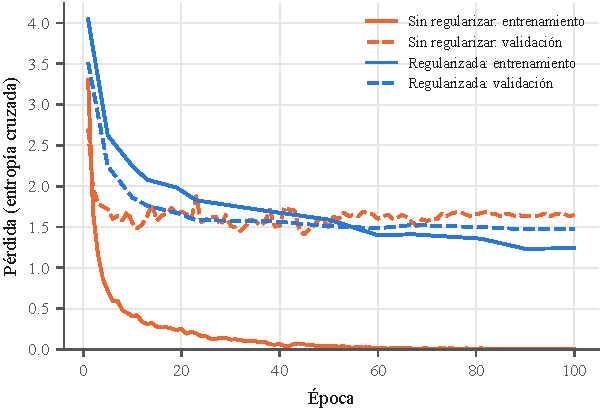
\includegraphics[width=0.75\textwidth]{fig_sobreajuste}
  \caption{Pérdida de entrenamiento y de validación de la CNN de audio sin
  regularización y con la regularización completa. Sin regularización la red
  memoriza el conjunto de entrenamiento y la pérdida de validación deja de
  bajar; con regularización ambas curvas se mantienen cercanas.}
  \label{fig:sobreajuste}
\end{figure}}{}

\begin{figure}[!htb]
  \centering
  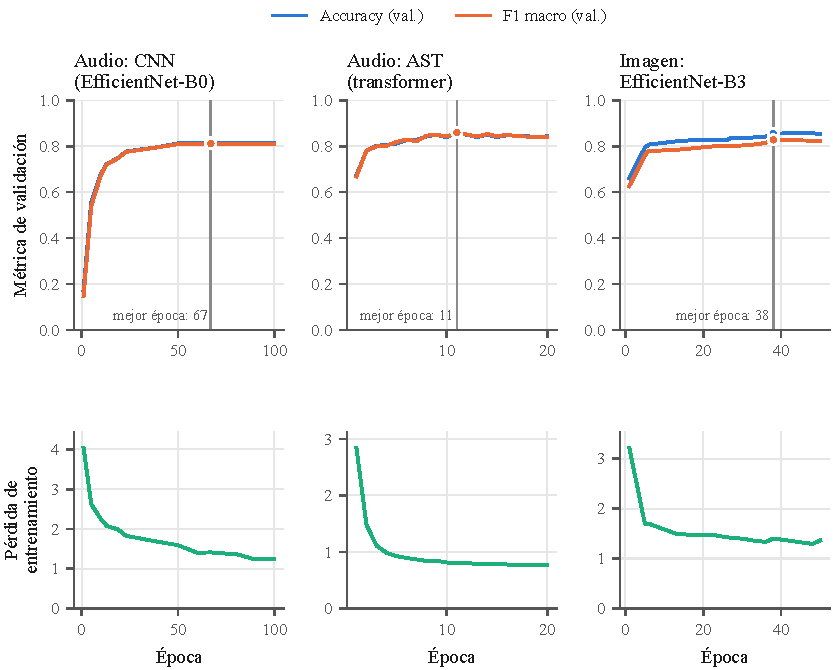
\includegraphics[width=\textwidth]{fig_curvas_entrenamiento}
  \caption{Curvas de entrenamiento de los tres clasificadores unimodales del sistema (CNN y AST de audio, EfficientNet-B3 de imagen): \textit{accuracy} y F1 macro en validación (arriba) y pérdida de
  entrenamiento (abajo). La línea vertical marca la época del mejor
  \textit{checkpoint}, que es el evaluado en prueba.}
  \label{fig:curvas}
\end{figure}

\subsection{Desempeño global}

La \tabref{tab:audio} y la \figref{fig:audio-cnn-ast} resumen el desempeño
en el conjunto de prueba (393 grabaciones, 55 especies). Ambos modelos
superan la meta de \SI{85}{\percent} de \textit{accuracy} con el protocolo
agregado y el AST supera a la CNN en los dos protocolos, con una diferencia
de dos puntos por ventana que se reduce a uno al agregar. La agregación por
grabación aporta entre 3,8 y 5,4 puntos sin reentrenar nada, porque promedia
ventanas sin vocalización o con ruido con las que sí contienen al ave focal.
Es la mitigación más barata del ruido de etiqueta de Xeno-canto descrito en
el \capref{cap:relacionado}. El costo del AST es alto: 86 millones de
parámetros frente a 4 millones, y 480 segundos por época frente a 22, es
decir, unas 20 veces más cómputo para un punto adicional de
\textit{accuracy}.

\begin{table}[!htb]
  \centering\small
  \caption{Clasificadores de audio en el conjunto de prueba (393 grabaciones,
  55 especies). El protocolo agregado promedia las probabilidades de hasta 12
  ventanas (CNN) u 8 (AST) de la grabación.}
  \label{tab:audio}
  \setlength{\tabcolsep}{4pt}\footnotesize
  \begin{tabular}{@{}l r r r r r r@{}}
    \toprule
    & \multicolumn{2}{c}{Ventana única} & \multicolumn{2}{c}{Agregado} & & \\
    \cmidrule(lr){2-3}\cmidrule(lr){4-5}
    Modelo & \textit{Accuracy} & F1 macro & \textit{Accuracy} & F1 macro & Parámetros & Tiempo/época \\
    \midrule
    EfficientNet-B0 sin regularizar & 0,735 & 0,736 & 0,789 & 0,784 & 4,1 M & \SI{22}{\second} \\
    EfficientNet-B0 regularizada & 0,812 & 0,811 & \textbf{0,858} & \textbf{0,858} & 4,1 M & \SI{22}{\second} \\
    AST (AudioSet) & 0,832 & 0,828 & \textbf{0,870} & \textbf{0,864} & 86,2 M & \SI{480}{\second} \\
    \bottomrule
  \end{tabular}
\end{table}

\begin{figure}[!htb]
  \centering
  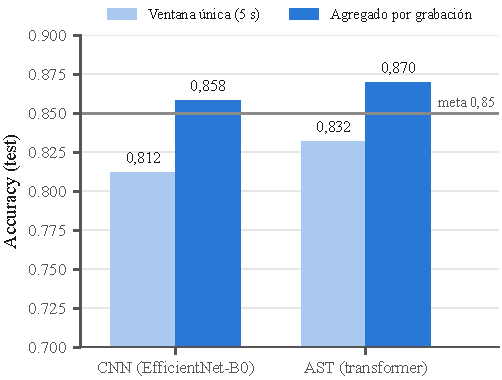
\includegraphics[width=0.6\textwidth]{fig_audio_cnn_vs_ast}
  \caption{\textit{Accuracy} en prueba de los clasificadores de audio con
  ventana única y con agregación por grabación.}
  \label{fig:audio-cnn-ast}
\end{figure}

La \tabref{tab:eval-extended} completa la caracterización con las métricas
que no dependen de un umbral de decisión. El AUC-ROC macro supera 0,99 en
los tres clasificadores del sistema y la especie correcta está entre las cinco más
probables en el \SI{97}{\percent} de las grabaciones (CNN) y el
\SI{95}{\percent} de las fotografías, lo que importa para un uso asistido en
que el sistema propone candidatas a un observador. La latencia mediana por
grabación, incluido el cálculo del espectrograma, es de \SI{18}{\milli\second}
para la CNN y \SI{177}{\milli\second} para el AST en la GPU del equipo. Una
fotografía con TTA tarda \SI{66}{\milli\second} (\SI{11}{\milli\second} con un
solo recorte).

\begin{table}[!htb]
  \centering\small
  \caption{Métricas extendidas de los clasificadores unimodales (solo audio o solo imagen) en el conjunto de prueba (protocolo operacional). AUC-ROC macro (cada especie frente a las demás); top-5: la especie correcta está entre las cinco más probables; latencia mediana por muestra en Apple M4 Pro (MPS), incluido el cálculo de características.}
  \label{tab:eval-extended}
  \footnotesize\setlength{\tabcolsep}{4pt}
  \begin{tabular}{@{}l r r r r r r@{}}
    \toprule
    Modelo & \textit{Accuracy} & F1 macro & AUC macro & Top-5 & Parámetros & Latencia (ms) \\
    \midrule
    Audio: CNN (agregado) & 0,858 & 0,858 & 0,991 & 0,969 & 4,1 M & 18 \\
    Audio: AST (agregado) & 0,870 & 0,864 & 0,993 & 0,949 & 86,2 M & 177 \\
    Imagen: B3 (TTA) & 0,848 & 0,808 & 0,990 & 0,948 & 10,8 M & 66 \\
    \bottomrule
  \end{tabular}
\end{table}


\textbf{Origen de la grabación.} Como el \SI{36}{\percent} del corpus
proviene de otros países, se evaluó por separado el desempeño sobre las 255
grabaciones chilenas y las 138 extranjeras del conjunto de prueba. La CNN
obtiene 0,847 de \textit{accuracy} en las chilenas y 0,877 en las
extranjeras (F1 macro 0,847 y 0,797). El AST obtiene 0,871 y 0,870. No hay,
por tanto, una penalización sobre las grabaciones chilenas: el desplazamiento de
dominio que se anticipó en el \capref{cap:datos} no se manifiesta en el
conjunto de prueba, en parte porque las grabaciones extranjeras pertenecen a
las mismas especies y a poblaciones vecinas (Argentina aporta la mitad de
ellas) y en parte porque el modelo aprende rasgos del canto más que del
ambiente de grabación.

\subsection{Desempeño por especie y por grupo de conservación}

La \figref{fig:f1-especie} (panel izquierdo) muestra el F1 de la CNN por
especie. Veintiséis especies superan 0,9 y solo ocho quedan bajo 0,7. La
\figref{fig:confusion} muestra en qué se equivoca el modelo y revela un
patrón distinto del esperado: los errores de audio \emph{no} se concentran
en pares de congéneres. De los 56 errores de la CNN en las 393 grabaciones,
solo tres ocurren entre especies del mismo género (\textit{Phrygilus gayi}
clasificado como \textit{P.~patagonicus}) y el resto se reparte en más de
cuarenta pares distintos, casi todos con un único caso. Las especies de peor
F1 (\textit{Cinclodes patagonicus} con 0,46, y \textit{Leptasthenura
aegithaloides}, \textit{Sylviorthorhynchus desmurii} y \textit{P.~gayi} con
0,62) fallan hacia una especie diferente en cada grabación, un patrón más
compatible con el ruido de etiqueta de Xeno-canto (especies de fondo, tramos
sin vocalización, llamados poco característicos) que con una similitud
acústica sistemática. El AST comete 51 errores con la misma dispersión. El
segundo factor es el \emph{tamaño del conjunto de prueba}: \textit{Agriornis
albicauda} (0,50) tiene tres grabaciones de prueba, de modo que un solo error
cuesta 33 puntos de \textit{recall}. La variabilidad de BirdNET entre
especies y contextos \citep{perezgranados2023birdnet} tiene aquí su
contraparte: el desempeño por especie depende tanto de la calidad de las
grabaciones disponibles como de la especie misma.

\begin{figure}[!htb]
  \centering
  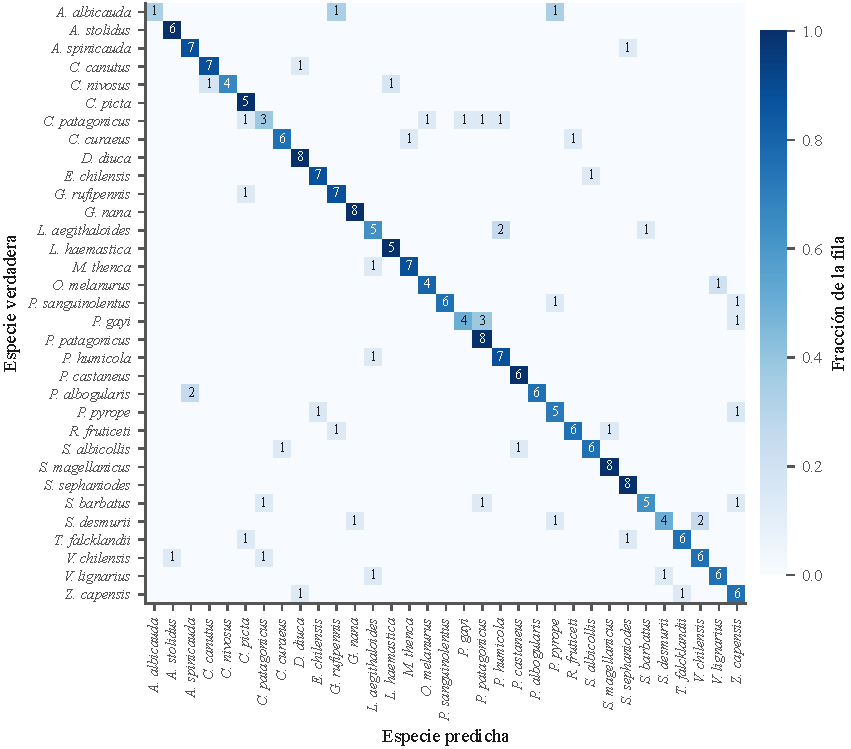
\includegraphics[width=0.9\textwidth]{fig_confusion_audio}
  \caption{Matriz de confusión de la CNN de audio (conjunto de prueba,
  agregado por grabación) restringida a las especies con \textit{recall}
  inferior a 0,8 y a las especies con que se confunden; el color indica la
  fracción de la fila y el número, las grabaciones. Los errores están
  dispersos: ningún par de especies acumula más de tres casos.}
  \label{fig:confusion}
\end{figure}

\begin{figure}[!htb]
  \centering
  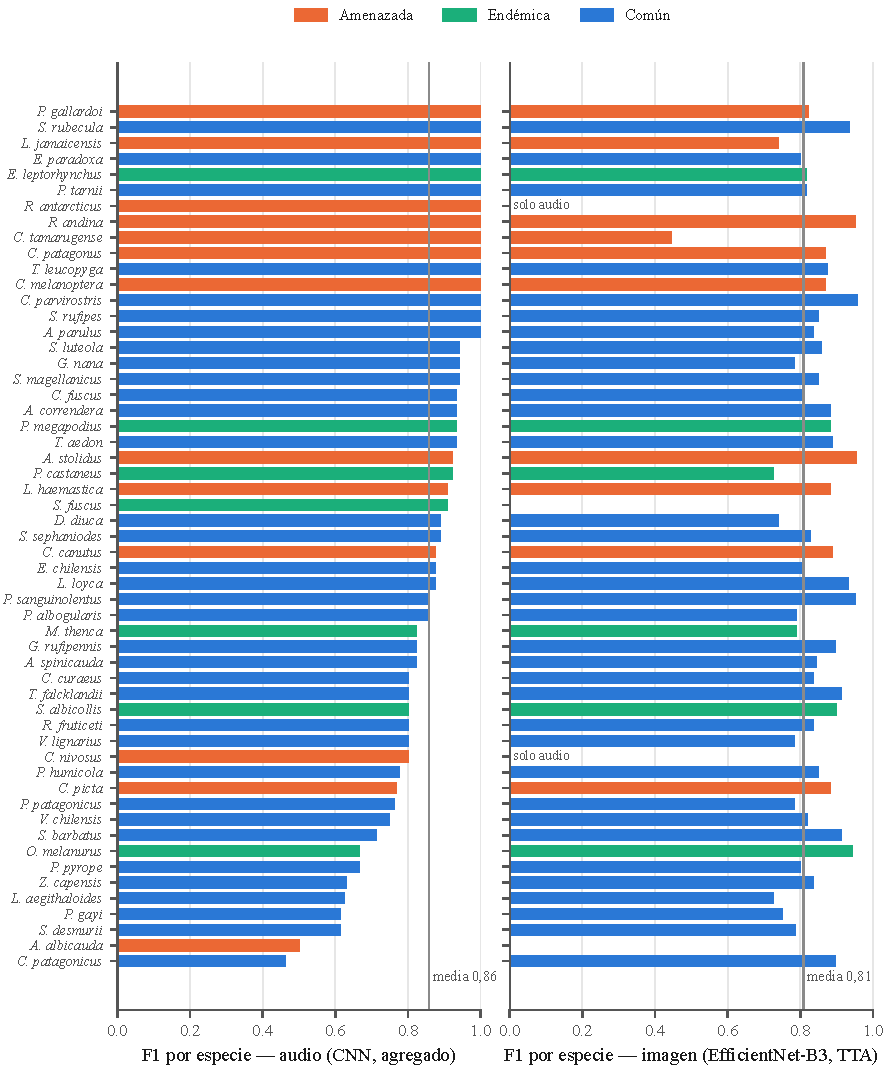
\includegraphics[width=\textwidth]{fig_f1_por_especie}
  \caption{F1 por especie en el conjunto de prueba del clasificador de audio
  (CNN, agregado por grabación) y del clasificador de imagen (EfficientNet-B3
  con TTA), coloreado por grupo de conservación y ordenado por el F1 de
  audio. Las dos especies sin fotografías suficientes no participan del
  clasificador de imagen.}
  \label{fig:f1-especie}
\end{figure}

Contra lo que la escasez de datos haría esperar, las especies amenazadas
obtienen en audio un F1 medio \emph{mayor} que las comunes, 0,906 frente a
0,838 (\tabref{tab:por-grupo}). Dos factores lo explican. Las amenazadas del conjunto son en su mayoría aves acuáticas, playeros y
loros, con vocalizaciones muy distintas de las de los paseriformes (el orden
de las aves cantoras, al que pertenece la mayoría de las especies pequeñas
del corpus), de modo que el problema \textit{fine-grained} es más fácil para
ellas. Además, sus conjuntos de prueba son pequeños, lo que hace sus métricas más altas pero también más inciertas. Las comunes, en cambio, concentran las especies de canto más variable y
las grabaciones más heterogéneas. El AST reparte el desempeño de forma más
pareja (F1 0,866, 0,896 y 0,857 en amenazadas, endémicas y comunes) y es el
mejor modelo en las endémicas. El desafío de la escasez de datos se
manifiesta, por tanto, menos en la métrica de prueba de las amenazadas que
en su variabilidad y en la dependencia de grabaciones extranjeras.

\begin{table}[!htb]
  \centering\small
  \caption{Desempeño por grupo de conservación. F1 medio por especie en el conjunto de prueba (audio: CNN, agregado por grabación; imagen: EfficientNet-B3 con TTA; fusión: pareo por especie) y AUC-ROC medio del SDM.}
  \label{tab:por-grupo}
  \fitwidth{\begin{tabular}{@{}l r r r r r r r@{}}
    \toprule
    Grupo & Especies & F1 audio & Especies & F1 imagen & F1 fusión & AUC MaxEnt & AUC RF \\
    \midrule
    Amenazada & 13 & 0,906 & 11 & 0,756 & 0,945 & 0,948 & 0,967 \\
    Endémica & 7 & 0,865 & 7 & 0,723 & 0,940 & 0,899 & 0,917 \\
    Común & 35 & 0,838 & 35 & 0,842 & 0,942 & 0,827 & 0,849 \\
    \midrule
    Todas & 55 & 0,858 & 53 & 0,808 & 0,942 & 0,863 & 0,884 \\
    \bottomrule
  \end{tabular}}
\end{table}


%-----------------------------------------------------------------------
\section{Identificación por imagen}\label{sec:res-imagen}

Se ajustó EfficientNet-B3 preentrenada en ImageNet, con entrada de
\SI{384}{px}, durante 50 épocas con la misma receta de regularización
(\textit{mixup}, suavizado de etiquetas, \textit{dropout}, profundidad
estocástica) y aumentación geométrica y de color. Una variante con pesos
NoisyStudent no mejoró la \textit{accuracy} (0,845 frente a 0,848), aunque sí
el F1 macro (0,820 frente a 0,808); se mantuvo la de ImageNet como rama del
sistema por su mejor \textit{accuracy} y porque la diferencia queda dentro del
intervalo de confianza. Una arquitectura mayor
(ConvNeXt preentrenada en ImageNet-21k) se descartó porque cada época tardaba
unas ocho horas en el equipo disponible, y ViT-B a \SI{384}{px}, comparable
a ConvNeXt, era inviable por el mismo motivo. Sí se entrenó la variante
pequeña de la familia, ViT-S/16 (21,7 M de parámetros, un cuarto de ViT-B;
preentrenado en ImageNet-21k y ajustado en ImageNet-1k), a \SI{224}{px}
durante 30 épocas (unos \SI{100}{\second} por época) con la misma receta de
regularización. Alcanzó 0,797 de \textit{accuracy} en validación, todavía
subiendo levemente al final, y 0,779 en prueba con recorte central (F1 macro
0,750), seis puntos por debajo de EfficientNet-B3 con el mismo protocolo
(0,839) y ocho con TTA, que al ViT lo empeora (0,767), posiblemente porque
sin la equivariancia de la convolución es más sensible al desplazamiento de
los recortes de esquina. El resultado es compatible con lo esperado para un
modelo con menos sesgos inductivos ajustado con unos pocos miles de
fotografías (\secref{sec:teoria-transformers}), pero la comparación está
confundida por la resolución (224 frente a \SI{384}{px}) y el número de
épocas, de modo que no permite concluir que la atención global no ayude
(\secref{sec:limitaciones}). A esta escala y con este cómputo, B3 sigue
siendo la rama de imagen del sistema. La \tabref{tab:imagen} resume los
resultados en las \num{1040} fotografías de prueba (53 especies).

\begin{table}[!htb]
  \centering\small
  \caption{Clasificadores de imagen en el conjunto de prueba (\num{1040}
  fotografías, 53 especies).}
  \label{tab:imagen}
  \begin{tabular}{@{}l r r r r r@{}}
    \toprule
    & \multicolumn{2}{c}{Recorte central} & \multicolumn{2}{c}{TTA (10 vistas)} & \\
    \cmidrule(lr){2-3}\cmidrule(lr){4-5}
    Modelo & \textit{Accuracy} & F1 macro & \textit{Accuracy} & F1 macro & Parámetros \\
    \midrule
    EfficientNet-B3 (ImageNet) & 0,839 & 0,802 & \textbf{0,848} & 0,808 & 10,8 M \\
    EfficientNet-B3 (NoisyStudent) & -- & -- & 0,845 & 0,820 & 10,8 M \\
    ViT-S/16 (ImageNet-21k, \SI{224}{px}) & 0,779 & 0,750 & 0,767 & 0,727 & 21,7 M \\
    \bottomrule
  \end{tabular}
\end{table}

El clasificador de imagen queda dos milésimas bajo la meta de 0,85 cuando se
evalúa solo. La curva de validación (\figref{fig:curvas}) muestra un
\textit{plateau} desde la época 36, de modo que más épocas no ayudan, y el
techo está en las especies difíciles: en el panel derecho de la
\figref{fig:f1-especie}, \textit{Scytalopus fuscus} (F1 0,00, cinco
fotografías de prueba) es visualmente casi idéntico a su congénere
\textit{S.~magellanicus}, y \textit{Agriornis albicauda} (0,00, dos
fotografías) y \textit{Conirostrum tamarugense} (0,44, tres) son las especies
con menos ejemplos. Diez especies superan 0,9. A diferencia del audio, en
imagen los errores sí se concentran en congéneres: el \SI{13}{\percent} de los
158 errores ocurre dentro de un género, y los pares más frecuentes son
\textit{Phrygilus gayi} y \textit{P.~patagonicus} (nueve casos en ambos
sentidos), los dos \textit{Scytalopus}, \textit{Pteroptochos castaneus} y
\textit{P.~tarnii}, y los dos \textit{Chloephaga}. También a diferencia del
audio, aquí las amenazadas y endémicas rinden peor que las comunes, con F1
medio de 0,756 y 0,723 frente a 0,842 (\tabref{tab:por-grupo}): en imagen la
escasez de
ejemplos pesa más que la distintividad, porque un plumaje se parece a otro
más de lo que un canto se parece a otro. Dado que la meta de
\SI{85}{\percent} se definió para el sistema multimodal, se aceptó este
resultado como la rama visual del sistema. La sección siguiente muestra que
la fusión la supera con amplitud.

%-----------------------------------------------------------------------
\section{Fusión multimodal}\label{sec:res-fusion}

\subsection{\textit{Late fusion} frente a cada modalidad}

La \textit{late fusion} combina las probabilidades de la CNN de audio (55 clases,
agregadas por grabación) y de EfficientNet-B3 (53 clases, proyectadas al
espacio de 55 con probabilidad cero para las dos especies que solo tienen audio) con
peso $\alpha = 0{,}5$ (Ecuación~\ref{eq:fusion}). Siguiendo el protocolo del
\capref{cap:teoria}, el pareo por especie se repitió 20 veces con semillas
distintas (30 pares por especie, \num{1590} pares por repetición, 53
especies) y se reportan la media y la desviación estándar
(\tabref{tab:fusion-summary}, \figref{fig:fusion}). Con la CNN como rama
de audio, la fusión alcanza \textbf{0,945 $\pm$ 0,004} de \textit{accuracy} y
0,942 $\pm$ 0,004 de F1 macro, frente a 0,865 $\pm$ 0,008 del audio solo y
0,816 $\pm$ 0,009 de la imagen sola sobre los mismos pares: 8,0 puntos sobre
la mejor modalidad y 12,9 sobre la imagen, con una variabilidad entre
repeticiones diez veces menor que la ganancia (el pareo único usado durante
el desarrollo había dado 0,950, dentro del rango). La meta del
\SI{85}{\percent} se supera con holgura y se confirma la hipótesis central
del Módulo 1.

\begin{table}[!htb]
  \centering\small
  \caption{\textit{Late fusion} evaluada con pareo por especie repetido: media y desviación estándar sobre 20 repeticiones de 1590 pares (53 especies), para las dos ramas de audio disponibles.}
  \label{tab:fusion-summary}
  \footnotesize
  \begin{tabular}{@{}l l r r@{}}
    \toprule
    Rama de audio & Modalidad & \textit{Accuracy} & F1 macro \\
    \midrule
    CNN (EfficientNet-B0) & Audio solo & 0,865 $\pm$ 0,008 & 0,861 $\pm$ 0,009 \\
    CNN (EfficientNet-B0) & Imagen sola & 0,816 $\pm$ 0,009 & 0,803 $\pm$ 0,009 \\
    CNN (EfficientNet-B0) & \textit{Late fusion} ($\alpha=0{,}5$) & 0,945 $\pm$ 0,004 & 0,942 $\pm$ 0,004 \\
    CNN (EfficientNet-B0) & Mejor fusión ($\alpha=0{,}5$, geométrica) & 0,956 $\pm$ 0,004 & 0,954 $\pm$ 0,004 \\
    AST & Audio solo & 0,877 $\pm$ 0,010 & 0,872 $\pm$ 0,010 \\
    AST & Imagen sola & 0,816 $\pm$ 0,009 & 0,803 $\pm$ 0,009 \\
    AST & \textit{Late fusion} ($\alpha=0{,}5$) & 0,946 $\pm$ 0,006 & 0,941 $\pm$ 0,006 \\
    AST & Mejor fusión ($\alpha=0{,}5$, geométrica) & 0,953 $\pm$ 0,005 & 0,948 $\pm$ 0,005 \\
    \bottomrule
  \end{tabular}
\end{table}


\begin{figure}[!htb]
  \centering
  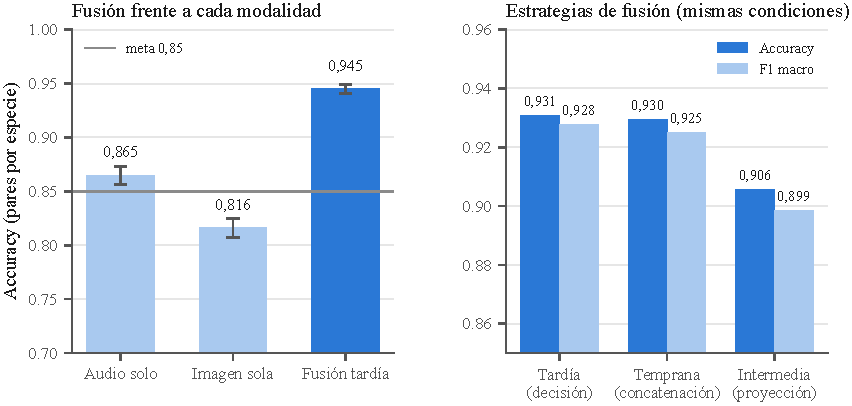
\includegraphics[width=\textwidth]{fig_fusion}
  \caption{Fusión multimodal evaluada con pareo por especie (\num{1590}
  pares, 53 especies). Izquierda: la \textit{late fusion} frente a cada modalidad
  sobre los mismos pares (media de 20 repeticiones; las barras de error,
  apenas visibles, son la desviación estándar). Derecha: comparación
  controlada de tres estrategias de fusión con cabezas entrenadas sobre los
  \textit{frozen embeddings} de ambos modelos.}
  \label{fig:fusion}
\end{figure}

El análisis de complementariedad explica la ganancia. En el
\SI{71,6}{\percent} de los pares ambas modalidades aciertan, en el
\SI{14,9}{\percent} solo el audio, en el \SI{10,0}{\percent} solo la imagen y
en el \SI{3,5}{\percent} ninguna. La fusión resuelve correctamente el
\SI{91,6}{\percent} de los pares en que las modalidades discrepan y no
estropea ninguno en que ambas aciertan: su techo, si resolviera todas las
discrepancias, sería 0,965, y alcanza 0,945. Cuando el audio confunde dos
\textit{Phrygilus}, la fotografía los separa. Cuando la imagen no distingue
dos \textit{Scytalopus}, el canto sí lo hace. El efecto es más visible por
grupo de conservación (\tabref{tab:por-grupo}): la fusión lleva a las
especies endémicas, las peores en imagen (F1 0,723) y medianas en audio
(0,865), a 0,940, y deja a los tres grupos entre 0,94 y 0,95. Con ello borra
la desventaja de las especies con menos datos.

\begin{figure}[!htb]
  \centering
  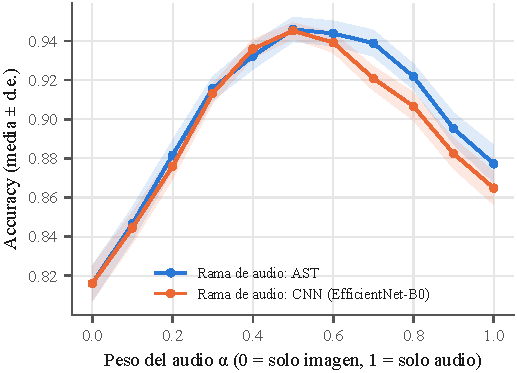
\includegraphics[width=0.6\textwidth]{fig_fusion_alpha}
  \caption{Sensibilidad de la \textit{late fusion} al peso del audio $\alpha$
  (media aritmética de probabilidades), con la CNN o el AST como rama de
  audio; banda: desviación estándar sobre 20 repeticiones del pareo.}
  \label{fig:fusion-alpha}
\end{figure}

La \figref{fig:fusion-alpha} muestra la sensibilidad al peso $\alpha$. La
curva es unimodal con máximo en $\alpha = 0{,}5$ y una meseta entre 0,4 y
0,6, y es asimétrica a favor del audio: con $\alpha = 0{,}7$ la fusión
todavía supera 0,92, mientras que con $\alpha = 0{,}3$ cae a 0,91. La media
geométrica de probabilidades (producto de expertos) mejora un punto sobre la
aritmética (0,956 $\pm$ 0,004) porque penaliza las clases que una modalidad
descarta con seguridad. Reemplazar la CNN por el AST en la rama de audio,
pese a sus 1,2 puntos adicionales en solitario (0,877 $\pm$ 0,010), no cambia
la fusión (0,946 $\pm$ 0,006): la ganancia proviene de la complementariedad,
no de la fuerza de cada rama. En síntesis, el sistema final usa la CNN como
rama de audio y \textit{late fusion} con $\alpha = 0{,}5$, que alcanza
0,945 $\pm$ 0,004 de \textit{accuracy} (intervalo de confianza al
\SI{95}{\percent} de 0,924 a 0,959). La variante con media geométrica es la
de mayor precisión observada (0,956 $\pm$ 0,004, con intervalo de 0,937 a
0,972). El sistema conserva la media aritmética por dos razones: los
intervalos de confianza de ambas variantes se solapan, y la media geométrica
anula cualquier especie a la que una rama asigne probabilidad cero, lo que
ocurre con las dos especies que solo tienen audio cuando la rama de imagen se
proyecta de 53 a 55 clases. La
diferencia entre usar la CNN o el AST como rama de audio (0,001) es menor
que una desviación estándar, de modo que no justifica un modelo veinte veces
más costoso.

\subsection{Comparación de estrategias de fusión}

Para aislar el efecto de la arquitectura de fusión se compararon las tres
estrategias de la taxonomía de \citet{baltrusaitis2019multimodal} en
condiciones idénticas: los mismos \textit{backbones} ya entrenados,
congelados como extractores de características (1\,280 dimensiones de audio y
1\,536 de imagen), los mismos pares por especie (150 de entrenamiento y 30 de
prueba por especie) y cabezas con la misma configuración (40 épocas, tasa de
aprendizaje $10^{-3}$, lotes de 64). La \textit{late fusion} entrena una cabeza
lineal por modalidad y promedia sus probabilidades. La \textit{early fusion}
concatena los dos \textit{embeddings} a la entrada de una única cabeza, y la
\textit{intermediate fusion} proyecta cada modalidad a un espacio común de 256
dimensiones antes de concatenar. El panel derecho de la \figref{fig:fusion}
muestra el resultado: la \textit{late fusion} (0,931) y la
\textit{early fusion} (0,930) empatan y la \textit{intermediate fusion} queda
por debajo
(0,906). Las proyecciones por modalidad agregan parámetros que sobreajustan
con los pares disponibles, y como los \textit{embeddings} ya son
representaciones de alto nivel, la transformación adicional no aporta. El
resultado respalda la elección de la \textit{late fusion} para el sistema final,
que además es robusta a modalidades faltantes. (El 0,945 de la subsección
anterior promedia los \textit{softmax} de los modelos completos, sin cabeza
adicional, por lo que es algo superior a las cabezas entrenadas sobre
\textit{frozen embeddings}.)

%-----------------------------------------------------------------------
\section{\textit{Baselines} de referencia}\label{sec:res-baselines}

Dos referencias sitúan el aporte de los modelos ajustados. La primera es la
de ``bajo costo'': un clasificador lineal sobre los \textit{frozen embeddings} de un modelo preentrenado, siguiendo el protocolo de
\citet{ghani2023embeddings}, con regresión logística multinomial y el
parámetro de regularización elegido en validación. Se usaron tres
extractores sin ajustar: EfficientNet-B0 de ImageNet sobre el espectrograma
log-mel, el AST de AudioSet (salida de 768 dimensiones) y EfficientNet-B3 de
ImageNet sobre la fotografía. La segunda referencia es un \emph{modelo de IA
generativa multimodal} (Claude, Anthropic;
\citealp{anthropic2026claude}) consultado mediante la API con cada
fotografía del conjunto de prueba y la lista cerrada de las 53 especies
candidatas, en modo \textit{zero-shot} (solo la lista) y \textit{few-shot}
(una fotografía de referencia por especie, tomada del conjunto de
entrenamiento). La respuesta se restringe a un nombre de la lista mediante
salida estructurada, de modo que el protocolo de métricas es el mismo del
clasificador propio.

\begin{table}[!htb]
  \centering\small
  \caption{\textit{Baselines} de referencia frente a los modelos ajustados (conjuntos de prueba). \textit{Frozen embeddings}: regresión logística sobre las representaciones de un modelo preentrenado sin ajustar. IA generativa: modelo de IA generativa multimodal consultado con la fotografía y la lista cerrada de especies.}
  \label{tab:baselines}
  \footnotesize
  \begin{tabularx}{\textwidth}{@{}l >{\raggedright\arraybackslash}X r r r@{}}
    \toprule
    Modalidad & Método & \textit{Accuracy} & F1 macro & AUC macro \\
    \midrule
    Audio & \textit{Frozen embeddings} de EfficientNet-B0 (ImageNet) + regresión logística & 0,547 & 0,545 & 0,901 \\
    Audio & \textit{Frozen embeddings} de AST (AudioSet) + regresión logística & 0,784 & 0,769 & 0,980 \\
    Imagen & \textit{Frozen embeddings} de EfficientNet-B3 (ImageNet) + regresión logística & 0,775 & 0,760 & 0,985 \\
    Imagen & IA generativa (claude-opus-5-5, \textit{zero-shot}, esfuerzo \textit{low}) & 0,803 & 0,765 & -- \\
    Imagen & IA generativa (claude-opus-5-5, \textit{few-shot}, esfuerzo \textit{low}) & 0,817 & 0,779 & -- \\
    \midrule
    Audio & \textbf{CNN EfficientNet-B0 ajustada (este trabajo)} & 0,858 & 0,858 & 0,991 \\
    Audio & \textbf{AST ajustado (este trabajo)} & 0,870 & 0,864 & 0,993 \\
    Imagen & \textbf{EfficientNet-B3 ajustada + TTA (este trabajo)} & 0,848 & 0,808 & 0,990 \\
    \bottomrule
  \end{tabularx}
\end{table}


\textbf{\textit{Frozen embeddings}.} Sobre el espectrograma, las características
de EfficientNet-B0 preentrenada en ImageNet, sin ajuste, llegan solo a
0,547 de \textit{accuracy} (\tabref{tab:baselines}): las representaciones
de imágenes naturales describen mal un espectrograma, y el ajuste completo
aporta 31 puntos. El AST preentrenado en AudioSet, un modelo de audio
general, transfiere mucho mejor (0,784 con una regresión logística) y el
ajuste agrega 8,6 puntos. El orden entre ambos extractores reproduce el
hallazgo de \citet{ghani2023embeddings} de que el preentrenamiento en el
dominio correcto importa más que la arquitectura. En imagen,
EfficientNet-B3 congelada da 0,775 y el ajuste suma 7,3 puntos. En las tres
ramas el AUC-ROC de la referencia congelada es alto (0,90 a 0,99): el
ordenamiento de candidatas es razonable sin ajustar, pero la decisión final
no lo es.

\textbf{IA generativa.} Claude Opus 5.5 identifica correctamente el
\SI{80,3}{\percent} de las \num{1040} fotografías de prueba en
\textit{zero-shot} (F1 macro 0,765), 4,5 puntos por debajo de
EfficientNet-B3 ajustada (0,848 de \textit{accuracy} y 0,808 de F1) y 14 por
debajo de la fusión multimodal. Cuatro fotografías fueron rechazadas por un
error de formato (archivos PNG con extensión JPEG, corregido en las corridas
posteriores) y cuentan como errores. La brecha entre su \textit{accuracy} y su F1 macro se explica por
cómo promedia cada métrica: la \textit{accuracy} cuenta aciertos sobre las
\num{1040} fotografías, donde pesan las especies comunes con 22 fotografías
de prueba, mientras que el F1 macro promedia el F1 de cada especie por
igual, de modo que las endémicas y las especies con dos o tres fotografías,
donde el modelo falla, pesan tanto como las comunes bien resueltas. El perfil por grupo es revelador: el modelo generativo
es excelente en las especies amenazadas (F1 0,839 y \SI{93}{\percent} de
acierto), que son aves acuáticas, playeros y loros abundantemente
fotografiados en todo el mundo, y competente en las comunes (0,795), pero
falla en las endémicas (F1 0,498 y \SI{56}{\percent} de acierto): confunde
sistemáticamente los tapaculos chilenos (turca 0,42, tapaculo 0,31, hued-hued
castaño 0,36, churrín del norte 0,25) y la chiricoca (0,40), especies que el
clasificador propio resuelve con F1 de 0,73 a 0,94. El modelo de IA generativa conoce las aves que el mundo fotografía y no las que solo Chile
tiene, que son justamente el foco de este trabajo. Supera al clasificador
especializado en 23 especies y pierde en 28. Su confianza declarada es
informativa (0,79 en los aciertos frente a 0,48 en los errores), lo que
permitiría abstenerse en los casos dudosos. El costo fue de US\$2,19 por el
conjunto completo (0,2 centavos por fotografía), con una latencia mediana de
\SI{2,4}{\second} por consulta frente a \SI{66}{\milli\second} del clasificador
propio en un equipo portátil.

En modo \textit{few-shot}, con una fotografía de referencia por especie
servida desde la caché de \textit{prompts}, el modelo sube a 0,817 de
\textit{accuracy} y 0,779 de F1 macro, sin respuestas inválidas. La mejora
se concentra donde faltaba conocimiento: las endémicas pasan de 0,498 a
0,567 de F1 (de \SI{56}{\percent} a \SI{71}{\percent} de acierto), con
ganancias de 14 a 27 puntos en la chiricoca, la turca y el tapaculo, mientras
que las amenazadas no cambian (0,837) y las comunes apenas (0,804). Una sola
fotografía de referencia cierra alrededor de un quinto de la brecha de las
endémicas respecto del clasificador propio, que sigue ganando en 29 especies
frente a 23, y el costo sube a US\$4,27 por el conjunto (0,4 centavos por
fotografía) con \SI{2,7}{\second} de latencia. La \figref{fig:llm-zero-few} resume el antes y el después por grupo. Ni en
\textit{zero-shot} ni en \textit{few-shot} el modelo generativo alcanza a la
rama de imagen ajustada con \num{4980} fotografías, y ambos quedan 13 puntos
por debajo de la fusión multimodal. La comparación responde el OE4 y, de
paso, justifica entrenar modelos propios para las especies que importan a la
conservación local.

\begin{figure}[!htb]
  \centering
  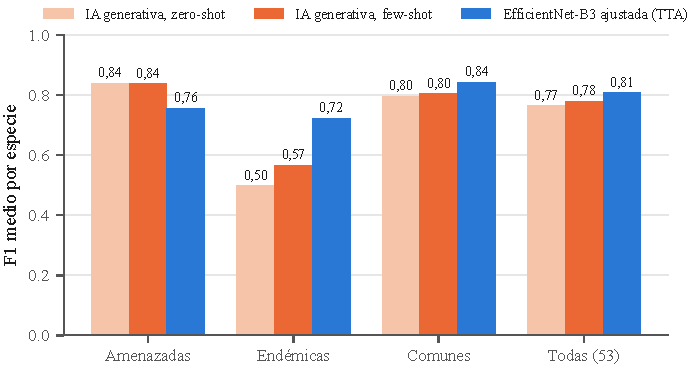
\includegraphics[width=0.8\textwidth]{fig_llm_zero_few}
  \caption{F1 medio por grupo de conservación del modelo generativo en
  \textit{zero-shot} y \textit{few-shot}, frente al clasificador de imagen
  ajustado. La fotografía de referencia mejora sobre todo a las endémicas, sin
  cerrar la brecha con el modelo propio.}
  \label{fig:llm-zero-few}
\end{figure}

%-----------------------------------------------------------------------
\section{Modelo de distribución espaciotemporal}\label{sec:res-sdm}

\subsection{Modelos comparados}

Sobre el conjunto de datos de la \secref{sec:datos-sdm} (presencias de cada
especie frente a \num{1500} puntos de fondo de grupo objetivo, muestreados
con la misma semilla para todos los modelos) se compararon cuatro
alternativas, cuyas bases se presentan en la \secref{sec:teoria-sdm}:
\begin{itemize}[leftmargin=*, itemsep=2pt]
  \item \textbf{MaxEnt} (\textit{baseline}): regresión logística penalizada
        con características lineales y cuadráticas y clases balanceadas,
        aprovechando la equivalencia entre MaxEnt y los modelos de regresión
        para datos de solo presencia \citep{fithian2013equivalence}.
  \item \textbf{Red neuronal conjunta}: el perceptrón multicapa multiespecie
        con dos capas ocultas de 64 unidades, \textit{dropout} de 0,3 y un
        \textit{embedding} de especie de 8 dimensiones, entrenado con entropía
        cruzada binaria ponderada durante 40 épocas sobre todas las especies a
        la vez.
  \item \textbf{Random Forest}: 300 árboles con clases balanceadas.
  \item \textbf{Gradient boosting}: 300 iteraciones con tasa de aprendizaje
        0,05 y clases balanceadas.
\end{itemize}
Todos usan las seis covariables (NDVI, temperatura, precipitación, elevación
y el mes cíclico) y se evalúan por especie con AUC-ROC sobre una partición
estratificada 70/30.

\begin{table}[!htb]
  \centering\small
  \caption{Modelos de distribución comparados: AUC-ROC medio sobre las 54 especies con al menos 20 presencias y número de especies en que cada modelo supera a MaxEnt. Partición aleatoria estratificada 70/30 y validación cruzada espacial por bloques de 200 km (5 \textit{folds}).}
  \label{tab:sdm-modelos}
  \footnotesize\setlength{\tabcolsep}{4pt}
  \fitwidth{\begin{tabular}{@{}l r r r r@{}}
    \toprule
    Modelo & AUC (aleatoria) & Gana a MaxEnt & AUC (espacial) & Gana a MaxEnt \\
    \midrule
    MaxEnt (regresión logística penalizada) & 0,863 & -- & 0,816 & -- \\
    Red neuronal conjunta & 0,856 & 15/54 & 0,810 & 21/54 \\
    Gradient boosting & 0,883 & 44/54 & 0,803 & 16/54 \\
    Random Forest & 0,884 & 46/54 & 0,812 & 17/54 \\
    \bottomrule
  \end{tabular}}
\end{table}


\begin{figure}[!htb]
  \centering
  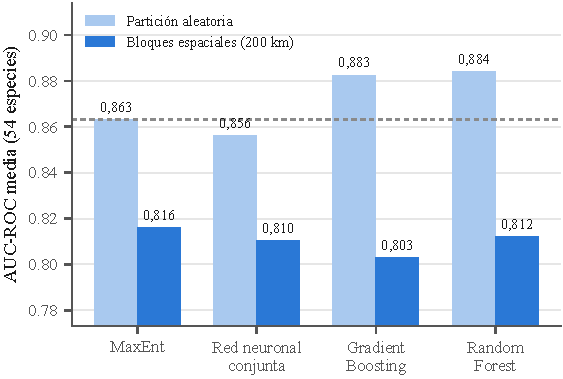
\includegraphics[width=0.62\textwidth]{fig_sdm_modelos}
  \caption{AUC-ROC medio de los modelos de distribución sobre las 54 especies
  modeladas. La línea punteada marca el \textit{baseline} MaxEnt.}
  \label{fig:sdm-modelos}
\end{figure}

El resultado (\tabref{tab:sdm-modelos}, \figref{fig:sdm-modelos}) contradice
la hipótesis original en su forma literal y la confirma en su espíritu. La
red neuronal \emph{no} supera a MaxEnt: obtiene 0,856 de AUC medio frente a
0,863 y solo gana en 15 de las 54 especies. Los ensambles de árboles, en
cambio, superan a MaxEnt con claridad: Random Forest alcanza 0,884 y gana en
46 de 54 especies, y gradient boosting 0,883 con 44 victorias. La mejora media de Random Forest sobre MaxEnt es de 0,021 (intervalo de
confianza al \SI{95}{\percent} de 0,015 a 0,027 y $p < 0{,}001$ en un test de
Wilcoxon pareado por especie), con casos de hasta siete puntos
(\textit{Vanellus chilensis} pasa de 0,725 a 0,795 y \textit{Limosa
haemastica} de 0,871 a 0,943) y ocho especies en que MaxEnt conserva una ventaja pequeña
(\figref{fig:sdm-especie}). La desventaja de la red neuronal también es
sistemática aunque pequeña (0,007 con $p = 0{,}001$). El patrón es coherente con la evidencia de que, en datos tabulares de
tamaño moderado, los modelos de árboles siguen superando a las redes
neuronales \citep{grinsztajn2022trees} y con los \textit{benchmarks} de SDM,
donde los árboles potenciados y los ensambles figuran entre los mejores
métodos.

\begin{figure}[!htb]
  \centering
  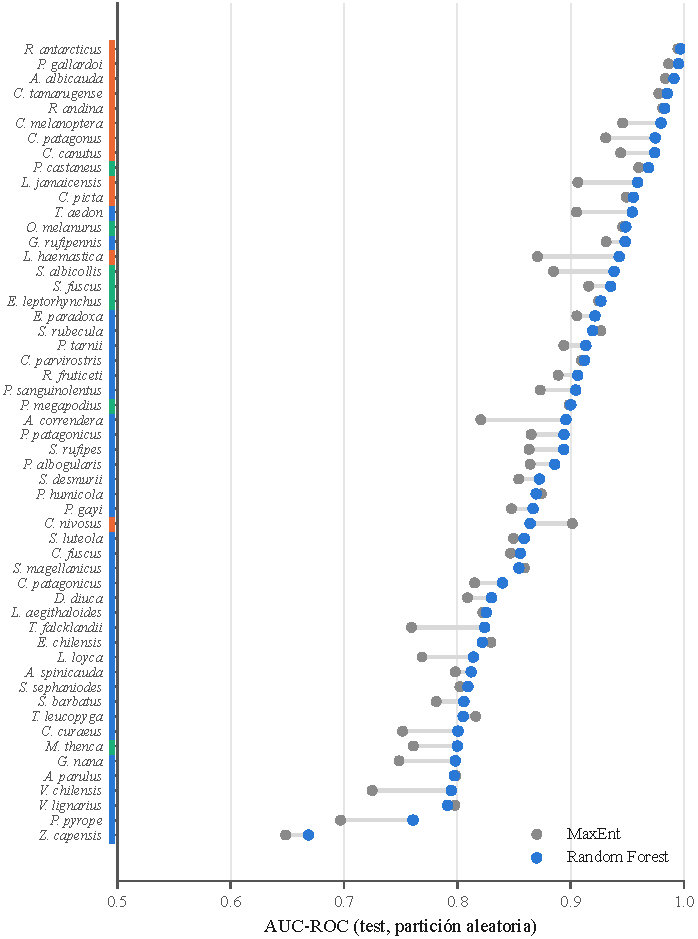
\includegraphics[width=0.78\textwidth]{fig_sdm_auc_especie}
  \caption{AUC-ROC por especie de MaxEnt y Random Forest (partición
  aleatoria), ordenadas por el valor de Random Forest; la franja de color
  indica el grupo de conservación.}
  \label{fig:sdm-especie}
\end{figure}

El desempeño por especie depende sobre todo de la amplitud de su
distribución. Las especies de rango restringido se modelan casi
perfectamente (\textit{Rallus antarcticus} 0,997, \textit{Podiceps gallardoi}
0,995, \textit{Agriornis albicauda} 0,991), mientras que los generalistas
ubicuos son los más difíciles (\textit{Zonotrichia capensis} 0,669,
\textit{Pyrope pyrope} 0,761): cuando una especie está en todas partes, el
fondo de grupo objetivo se parece a sus presencias y las covariables no
pueden separarlos. Por eso, al contrario del clasificador de imagen, aquí las
especies amenazadas obtienen el AUC más alto, 0,967 con Random Forest frente
a 0,849 de las comunes (\tabref{tab:por-grupo}): la escasez de registros no
impide modelarlas, porque sus pocos registros son ambientalmente muy
informativos.

\subsection{¿Aportan los datos satelitales no estructurados?}

Para dar al aprendizaje profundo una ventaja que MaxEnt no puede aprovechar,
se probaron dos fuentes de información satelital no estructurada
(\figref{fig:sdm-satelite}, panel izquierdo). Con parches de cobertura de
suelo de \SI{3}{\kilo\metre} procesados por una CNN junto a las covariables,
la red cayó a 0,613 de AUC, y con el \textit{embedding} satelital de 64
dimensiones de AlphaEarth, a 0,767. Se verificó que los parches estaban
correctamente alineados, de modo que la degradación no es un error de datos
sino sobreajuste: la cobertura de suelo es redundante con el NDVI y la
elevación (bosque donde el NDVI es alto, suelo desnudo donde es bajo o la
altitud es alta) y la capacidad adicional de la red solo agrega varianza.
La prueba definitiva es que el \textit{embedding} también perjudica a los
árboles, que son robustos a características irrelevantes: Random Forest baja
de 0,884 a 0,878 (una caída pequeña pero consistente en 44 de 54 especies,
$p < 0{,}001$) y gradient boosting de 0,883 a 0,881.

\begin{figure}[!htb]
  \centering
  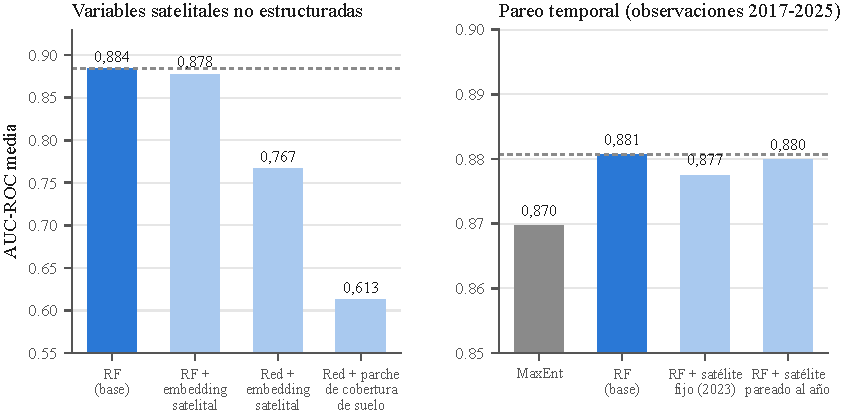
\includegraphics[width=\textwidth]{fig_sdm_satelite}
  \caption{Experimentos con información satelital. Izquierda: AUC-ROC medio
  al agregar el \textit{embedding} satelital o parches de cobertura de suelo
  a las covariables base. Derecha: pareo temporal del \textit{embedding}
  satelital al año de cada observación, sobre el subconjunto 2017--2025 (53
  especies).}
  \label{fig:sdm-satelite}
\end{figure}

Quedaba una explicación alternativa: el desajuste temporal entre la imagen
satelital (un compuesto fijo de 2023) y observaciones de cualquier año. Para
descartarla se repitió el experimento sobre las observaciones de 2017 a
2025, pareando a cada punto el NDVI y el \textit{embedding} del año en que
fue observado (panel derecho de la \figref{fig:sdm-satelite}). El pareo ayuda marginalmente respecto del compuesto fijo (0,880 frente a
0,877 y mejor en 32 de 53 especies, $p = 0{,}010$), lo que confirma que el
desajuste existía, pero ninguna versión supera a las covariables base sin
satélite (0,881): la diferencia entre el satélite pareado y la base es
$-0{,}001$ con un intervalo de confianza de $-0{,}005$ a $+0{,}003$ ($p =
0{,}89$), es decir, indistinguible de cero (\tabref{tab:tests-sdm}; el test
se hace sobre Random Forest, el mejor modelo del bloque). El
desajuste temporal era un factor menor. La causa es la redundancia.

\subsection{Validación espacial por bloques}

Para comprobar que la comparación anterior no está inflada por la
autocorrelación espacial, se repitió con validación cruzada por bloques,
siguiendo el protocolo de \texttt{blockCV} \citep{valavi2019blockcv}. Los
semivariogramas empíricos de las covariables dan rangos de autocorrelación
de \SI{650}{\kilo\metre} (NDVI, precipitación) a \SI{1200}{\kilo\metre}
(temperatura, elevación), consecuencia del gradiente latitudinal de Chile.
Bloques de ese tamaño dejarían entre cuatro y seis en todo el país,
de modo que se usaron bloques de \SI{200}{\kilo\metre} (46 bloques),
asignados al azar a cinco \textit{folds} equilibrados en número de
registros: de 10\,700 a 17\,400 filas por \textit{fold} del conjunto apilado
por especie (presencias más los 1\,500 puntos de fondo de cada especie, que
se repiten entre especies), equivalentes a entre unos 5\,800 y 8\,900 de los
34\,926 puntos distintos. Cada modelo se
entrena en cuatro \textit{folds} y se evalúa en el quinto, con los mismos
puntos y el mismo fondo que la partición aleatoria. En 13 especies de rango
restringido, cuyas presencias caen en pocos bloques, solo dos a cuatro
\textit{folds} tienen presencias suficientes para calcular el AUC.

El resultado (\tabref{tab:sdm-modelos}, \figref{fig:sdm-modelos}) cambia la
lectura. Todos los modelos caen entre cinco y ocho puntos al extrapolar a
bloques no vistos (MaxEnt de 0,863 a 0,816, Random Forest de 0,884 a 0,812,
gradient boosting a 0,803 y la red a 0,810) y las diferencias entre ellos
quedan dentro de la variabilidad entre \textit{folds} (desviación estándar
media de 0,06). Random Forest supera a MaxEnt en solo 17 de las 54 especies, la diferencia
media es de $-0{,}004$ con un intervalo de confianza que incluye el cero (de
$-0{,}013$ a $+0{,}004$, con $p = 0{,}06$) y en 21 especies es menor que 0,01.
Por grupo, los árboles conservan
ventaja en las especies amenazadas (0,901 frente a 0,883) y la pierden en
las comunes (0,779 frente a 0,788) y endémicas (0,823 frente a 0,845). La
ventaja de los ensambles de árboles es, por tanto, una ventaja de
\emph{interpolación}: con registros en todo el territorio aprovechan
interacciones locales entre covariables que MaxEnt no modela, pero al
predecir en zonas sin registros las funciones de respuesta suaves de MaxEnt
generalizan igual o mejor. Para la pregunta de investigación esto significa
que el aprendizaje automático supera a MaxEnt en el uso habitual de un SDM
(describir la distribución donde hay datos), pero no al extrapolar a
regiones sin muestreo, que es el escenario que la validación por bloques
simula y el más exigente. La \tabref{tab:tests-sdm} reúne todas las
comparaciones pareadas de este capítulo.

\begin{table}[!htb]
  \centering\footnotesize
  \caption{Comparaciones pareadas por especie entre modelos de distribución: diferencia media de AUC-ROC con intervalo \textit{bootstrap} al \SI{95}{\percent}, número de especies en que el primer modelo supera al segundo y valor $p$ del test de Wilcoxon de rangos con signo (bilateral).}
  \label{tab:tests-sdm}
  \begin{tabular}{@{}l l r r r r@{}}
    \toprule
    Protocolo & Comparación & $n$ & $\Delta$AUC [IC 95\,\%] & Gana & $p$ \\
    \midrule
    aleatoria & Random Forest vs. MaxEnt & 54 &  0,021 [0,015; 0,027] & 46/54 & $<$0,001 \\
    aleatoria & Gradient boosting vs. MaxEnt & 54 &  0,019 [0,012; 0,026] & 44/54 & $<$0,001 \\
    aleatoria & Red neuronal vs. MaxEnt & 54 & -0,007 [-0,011; -0,003] & 15/54 & 0,001 \\
    aleatoria & RF + \textit{embedding} satelital vs. RF & 54 & -0,006 [-0,009; -0,004] & 10/54 & $<$0,001 \\
    espacial & Random Forest vs. MaxEnt & 54 & -0,004 [-0,012; 0,004] & 17/54 & 0,060 \\
    espacial & Gradient boosting vs. MaxEnt & 54 & -0,013 [-0,022; -0,004] & 16/54 & 0,003 \\
    espacial & Red neuronal vs. MaxEnt & 54 & -0,006 [-0,012; 0,000] & 21/54 & 0,044 \\
    temporal 2017-2025 & RF vs. MaxEnt & 53 &  0,011 [0,005; 0,017] & 38/53 & $<$0,001 \\
    temporal 2017-2025 & RF + satélite fijo vs. RF & 53 & -0,003 [-0,007; 0,000] & 21/53 & 0,069 \\
    temporal 2017-2025 & RF + satélite pareado vs. RF & 53 & -0,001 [-0,005; 0,003] & 28/53 & 0,891 \\
    temporal 2017-2025 & RF + satélite pareado vs. fijo & 53 &  0,002 [0,001; 0,004] & 32/53 & 0,010 \\
    \bottomrule
  \end{tabular}
\end{table}


\subsection{Mapas de distribución estimada}

La \figref{fig:sdm-mapas} muestra la probabilidad de presencia estimada por
Random Forest sobre la grilla de \SI{0,1}{\degree} para tres especies de
distribución contrastante: el chucao, propio del bosque templado lluvioso
del sur; el tricahue (EN), confinado a los valles del centro-norte; y el
comesebo de los tamarugales (EN), restringido a la Pampa del Tamarugal. En
los tres casos el mapa reproduce el rango conocido y los avistamientos caen
en las zonas de alta probabilidad, sin que el modelo haya recibido las
coordenadas como covariable: la distribución emerge del clima, la vegetación
y la elevación. La \figref{fig:sdm-estacional} ilustra el eje temporal con el
zarapito de pico recto (VU), un playero migratorio que pasa el verano austral
en Chile: el modelo asigna alta probabilidad a los humedales del sur en enero
y la reduce en julio, cuando la especie está en el hemisferio norte, aunque
con la salvedad de que la mitad de los registros se concentra en verano por
el propio esfuerzo de observación.

\begin{figure}[!htb]
  \centering
  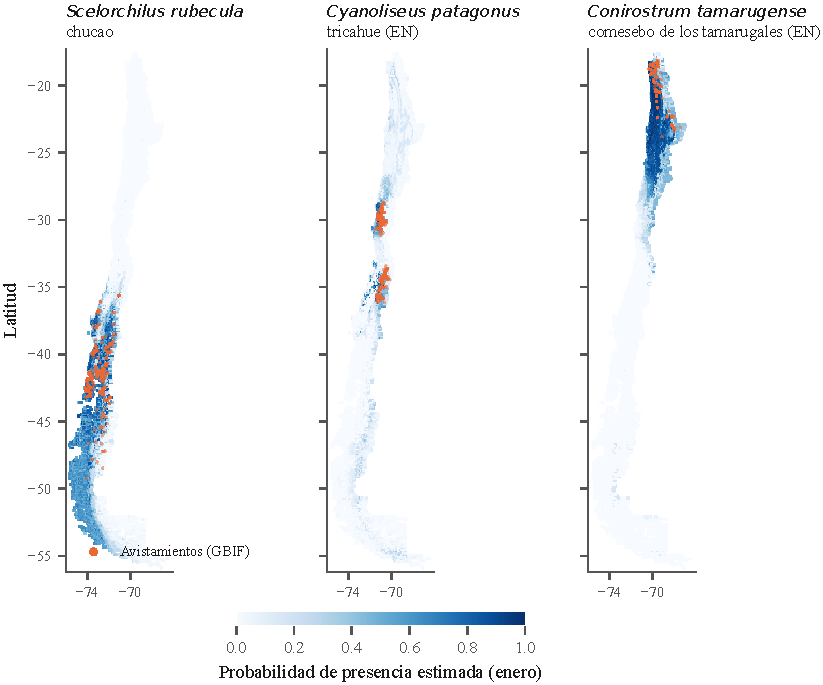
\includegraphics[width=\textwidth]{fig_sdm_mapas}
  \caption{Probabilidad de presencia en enero estimada por Random Forest para
  tres especies de distribución contrastante, con una muestra de sus
  avistamientos superpuesta.}
  \label{fig:sdm-mapas}
\end{figure}

\begin{figure}[!htb]
  \centering
  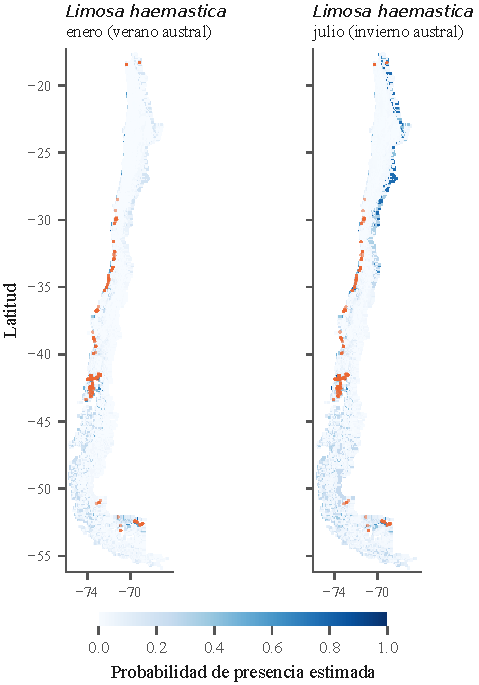
\includegraphics[width=0.62\textwidth]{fig_sdm_estacional}
  \caption{Eje temporal del modelo: probabilidad de presencia estimada para
  \textit{Limosa haemastica} en enero y en julio.}
  \label{fig:sdm-estacional}
\end{figure}

%-----------------------------------------------------------------------
\section{Prototipo integrado}\label{sec:prototipo}

Los tres modelos se integraron en un prototipo web construido con
Streamlit. El usuario sube una grabación y/o una fotografía. El sistema
calcula las probabilidades de cada rama disponible, las fusiona si hay
ambas, muestra las cinco especies más probables con su confianza y su
categoría de conservación, y dibuja sobre un mapa interactivo la
distribución estimada de la especie identificada para el mes elegido, usando
los Random Forest por especie entrenados con todos los datos y la grilla de
covariables precalculada. La inferencia completa tarda unos segundos en CPU.
El prototipo cumple el papel de ``despliegue'' de CRISP-DM en su forma
mínima: demuestra que los módulos funcionan juntos de extremo a extremo con
entradas reales, aunque no es un servicio productivo
(\capref{cap:conclusiones}).

%-----------------------------------------------------------------------
\section{Síntesis frente a los objetivos}\label{sec:sintesis}

La \tabref{tab:sintesis} resume el estado de cada objetivo específico, la
\tabref{tab:ic} reúne los intervalos de confianza de las métricas principales
y la \tabref{tab:costo} el costo computacional de los modelos, que completa
la documentación que pide el OE5.

\begin{table}[!htb]
  \centering\footnotesize
  \caption{Intervalos de confianza al \SI{95}{\percent} de las métricas principales de identificación. \textit{Bootstrap} percentil con \num{2000} remuestreos de las muestras de prueba (fusión: 300 remuestreos estratificados por especie de grabaciones y fotografías, con el pareo recalculado); los \textit{baselines} de \textit{frozen embeddings} usan el intervalo normal de una proporción.}
  \label{tab:ic}
  \begin{tabular}{@{}l r r r@{}}
    \toprule
    Modelo & $n$ & \textit{Accuracy} [IC 95\,\%] & F1 macro [IC 95\,\%] \\
    \midrule
    Audio: CNN EfficientNet-B0 (agregado) & 393 & 0,858 [0,822; 0,891] & 0,858 [0,804; 0,880] \\
    Audio: AST (agregado) & 393 & 0,870 [0,837; 0,903] & 0,864 [0,811; 0,889] \\
    Imagen: EfficientNet-B3 (TTA) & 1040 & 0,848 [0,826; 0,869] & 0,808 [0,779; 0,827] \\
    IA generativa \textit{zero-shot} & 1040 & 0,803 [0,779; 0,828] & 0,765 [0,733; 0,787] \\
    IA generativa \textit{few-shot} & 1040 & 0,817 [0,793; 0,840] & 0,779 [0,748; 0,801] \\
    \textit{Frozen embeddings}: EfficientNet-B0 (ImageNet) & 393 & 0,547 [0,498; 0,596] & 0,545 \\
    \textit{Frozen embeddings}: AST (AudioSet) & 393 & 0,784 [0,743; 0,824] & 0,769 \\
    \textit{Frozen embeddings}: EfficientNet-B3 (ImageNet) & 1040 & 0,775 [0,750; 0,800] & 0,760 \\
    Pareo: audio solo & 1590 & 0,861 [0,827; 0,893] & -- \\
    Pareo: imagen sola & 1590 & 0,819 [0,792; 0,847] & -- \\
    Pareo: \textit{late fusion} ($\alpha = 0{,}5$) & 1590 & 0,942 [0,924; 0,959] & -- \\
    Pareo: \textit{late fusion} geométrica & 1590 & 0,955 [0,937; 0,972] & -- \\
    \bottomrule
  \end{tabular}
\end{table}


\begin{table}[!htb]
  \centering\footnotesize
  \caption{Cumplimiento de los objetivos específicos.}
  \label{tab:sintesis}
  \begin{tabularx}{\textwidth}{@{}>{\raggedright\arraybackslash}p{3.3cm} X >{\raggedright\arraybackslash}p{2.4cm}@{}}
    \toprule
    Objetivo & Resultado & Estado \\
    \midrule
    OE1 Conjunto de datos reproducible & Tres corpus (\num{2508} grabaciones, \num{7060} fotografías, \num{100270} registros) con particiones sin fuga y \textit{scripts} reanudables & Cumplido \\
    OE2 Clasificadores y fusión, \textit{accuracy} $>$ \SI{85}{\percent} en $\geq 50$ especies & Audio 0,858 (CNN) y 0,870 (AST) sobre 55 especies; imagen 0,848; fusión 0,945 $\pm$ 0,004 sobre 53 especies & Cumplido \\
    OE3 SDM frente a MaxEnt & Random Forest 0,884 $>$ MaxEnt 0,863 (46/54 especies) con partición aleatoria; bajo validación espacial todos los modelos empatan (0,80--0,82); la red neuronal no supera a MaxEnt en ningún protocolo & Cumplido (hallazgo matizado) \\
    OE4 Comparación con IA generativa & \textit{Zero-shot} 0,803 y \textit{few-shot} 0,817, frente a 0,848 del clasificador propio y 0,945 de la fusión; falla en las endémicas & Cumplido \\
    OE5 Documentación de desempeño y limitaciones & Métricas, costo computacional, análisis por especie, grupo y origen; limitaciones en el \capref{cap:conclusiones} & Cumplido \\
    \bottomrule
  \end{tabularx}
\end{table}

\begin{table}[!htb]
  \centering\small
  \caption{Costo computacional de los modelos en Apple M4 Pro (MPS). El ViT-S/16
  se entrenó solo como comparación.}
  \label{tab:costo}
  \footnotesize\setlength{\tabcolsep}{4pt}
  \fitwidth{\begin{tabular}{@{}l r r r r@{}}
    \toprule
    Modelo & Parámetros & Entrenamiento (total) & Épocas & Inferencia (mediana) \\
    \midrule
    Audio: EfficientNet-B0 & 4,1 M & \SI{22}{\second}/época (\SI{37}{\minute}) & 100 & \SI{18}{\milli\second} por grabación \\
    Audio: AST & 86,2 M & \SI{480}{\second}/época (\SI{2,7}{\hour}) & 20 & \SI{177}{\milli\second} por grabación \\
    Imagen: EfficientNet-B3 & 10,8 M & 250--\SI{500}{\second}/época (3,5--\SI{7}{\hour}) & 50 & \SI{66}{\milli\second} por foto (TTA) \\
    Imagen: ViT-S/16 (\SI{224}{px}) & 21,7 M & \SI{101}{\second}/época (\SI{50}{\minute}) & 30 & -- \\
    SDM: Random Forest & 300 árboles/especie & segundos por especie & -- & $<$\SI{1}{\second} por mapa \\
    SDM: red conjunta & $\approx$ \num{5600} & $\approx$ \SI{1}{\minute} & 40 & -- \\
    \bottomrule
  \end{tabular}}
\end{table}


\chapter{Conclusiones, desafíos y trabajo futuro}\label{cap:conclusiones}
%=======================================================================
% cap6_conclusiones.tex — Conclusiones, desafíos y trabajo futuro
%=======================================================================

%-----------------------------------------------------------------------
\section{Respuesta a las preguntas de investigación}\label{sec:respuestas}

\textbf{PI1. ¿Puede un sistema multimodal identificar aves chilenas mejor
que los clasificadores unimodales (solo audio o solo imagen) y que un modelo de IA generativa multimodal?} Sí, en ambas comparaciones. La \textit{late fusion} de audio e imagen alcanza 0,945 $\pm$ 0,004 de
\textit{accuracy} sobre 53 especies (intervalo de confianza al
\SI{95}{\percent} de 0,924 a 0,959), 8,0 puntos más que el mejor
clasificador unimodal sobre los mismos pares y casi 10 sobre la
meta comprometida, y lo hace con datos no emparejados de ciencia ciudadana,
un escenario que la literatura previa no había explorado. Cada modalidad
por separado también cumple o roza la meta: audio 0,858 (CNN) y 0,870 (AST)
sobre 55 especies, imagen 0,848 sobre 53. Frente al modelo de IA generativa multimodal, el sistema especializado gana con claridad: Claude Opus 5.5 alcanza 0,803 en \textit{zero-shot} y 0,817 en
\textit{few-shot} sobre las mismas fotografías, 3 a 4,5 puntos menos que la
rama de imagen y 13 menos que la fusión, y falla precisamente en las
especies endémicas chilenas (F1 0,498 y 0,567 frente a 0,940 de la
fusión).

\textbf{PI2. ¿Puede un SDM basado en aprendizaje automático superar a
MaxEnt?} Sí, pero no con redes neuronales. Random Forest y gradient
boosting superan a MaxEnt en AUC-ROC (0,884 y 0,883 frente a 0,863) en 46 y 44
de las 54 especies, mientras que la red neuronal conjunta queda por debajo
(0,856) y la incorporación de parches de cobertura de suelo y
\textit{embeddings} de imágenes satelitales de un modelo fundacional degrada
a todos los modelos. La hipótesis ``aprendizaje
profundo $>$ MaxEnt'' se refuta con evidencia. La hipótesis ``aprendizaje
automático $>$ MaxEnt'' se confirma con un método más simple, pero con una
condición importante: bajo validación espacial por bloques, que mide la
extrapolación a zonas sin registros, todos los modelos caen a 0,80--0,82 y
ninguno supera a MaxEnt. El aprendizaje automático gana al interpolar, no al
extrapolar.

\textbf{PI3. ¿Cómo afecta la escasez de datos de las especies amenazadas y
qué estrategias la mitigan?} De forma distinta en cada módulo. En imagen,
donde los plumajes de congéneres se parecen, las especies con menos
fotografías son las que fallan (F1 medio 0,756 en amenazadas frente a 0,842
en comunes) y dos quedaron fuera del clasificador. En audio, la escasez se
mitigó con grabaciones de otras poblaciones, aumentación en el espectrograma
y pesos por clase, y las amenazadas rinden incluso mejor que las comunes
(0,906 frente a 0,838) porque sus vocalizaciones son distintivas. El precio
es la dependencia de audio extranjero y conjuntos de prueba de tres a ocho
grabaciones. En distribución, los pocos registros de las especies de rango
restringido bastan para modelarlas casi perfectamente (AUC 0,967). La fusión
multimodal es, en sí misma, la mitigación más efectiva: cubre las especies
que una modalidad no puede clasificar y corrige los errores de la otra.

%-----------------------------------------------------------------------
\section{Discusión}\label{sec:discusion}

\textbf{Por qué funciona la fusión.} La complementariedad no es casual. El
audio separa especies por estructura temporal y espectral del canto, que en
aves es un carácter de reconocimiento de especie. La imagen separa por forma
y plumaje. Los pares que confunde una modalidad (\textit{Cinclodes} y
\textit{Phrygilus} en audio, \textit{Scytalopus} en imagen) son distintos de
los que confunde la otra, y la \textit{late fusion} solo necesita que una de las dos
esté segura. Que la \textit{late fusion} y la \textit{early fusion} empaten y
la \textit{intermediate fusion} pierda indica que, con \textit{backbones}
fuertes y pocos pares, lo simple gana: la forma más barata de combinar
evidencia es también la mejor, y la \textit{late fusion} tiene la ventaja de
operar con una sola modalidad.

\textbf{Por qué los árboles ganan al aprendizaje profundo en el SDM.} El
problema de distribución, tal como se formuló, es tabular: seis covariables
y unos cientos de presencias por especie. En ese régimen los ensambles de
árboles tienen sesgos inductivos adecuados (invariancia a la escala de las
variables, fronteras de decisión irregulares, robustez a variables
irrelevantes) y las redes necesitan más datos o regularización
\citep{grinsztajn2022trees}. La red conjunta comparte información entre
especies, pero esa ventaja no compensa la pérdida frente a 300 árboles por
especie. Los experimentos satelitales muestran además que la señal
ambiental relevante ya está en las covariables clásicas: el NDVI, el clima y
la elevación resumen lo que la cobertura de suelo y el \textit{embedding}
satelital repiten con más ruido. Y la validación espacial agrega
un matiz: la ventaja de los árboles es de interpolación. Al extrapolar a
zonas sin registros, la respuesta suave y regularizada de MaxEnt generaliza
igual de bien. Este resultado es informativo para la práctica: con buenas
covariables, un Random Forest es la elección razonable para describir la
distribución donde hay datos, MaxEnt sigue siendo tan bueno como cualquiera
para proyectarla a zonas sin muestreo, y la complejidad adicional debe
justificarse con una ganancia medida, no supuesta.

\textbf{El valor de la agregación y de los protocolos operacionales.} La
métrica por ventana única subestima el desempeño real en cuatro puntos.
Evaluar como se usará el sistema (la grabación completa, la fotografía con
TTA, el par audio-imagen) no solo da números más altos sino más honestos
respecto del caso de uso. Lo mismo vale para la comparación de costo: el AST
mejora un punto a la CNN con veinte veces el cómputo, una diferencia que
decide qué modelo conviene desplegar en un dispositivo de campo.

\textbf{Relación con la literatura.} La ganancia de la fusión coincide con lo
observado en SSW60, donde combinar audio e imagen supera a cada modalidad
\citep{vanhorn2022ssw60}, y la extiende a datos no emparejados de ciencia
ciudadana. En distribución, el resultado es coherente con el
\textit{benchmark} de \citet{valavi2022benchmark}, donde MaxEnt y los
ensambles de árboles quedan entre los mejores métodos con diferencias
pequeñas, y con la advertencia de \citet{roberts2017crossvalidation}: la
partición aleatoria sobreestima el desempeño cuando los datos tienen
estructura espacial, aquí entre cinco y ocho puntos de AUC. Por último, el
desempeño de la rama de audio sobre especies chilenas, frente a la cobertura
moderada de BirdNET en Sudamérica \citep{funosas2026birdnet}, respalda la
estrategia de entrenar clasificadores regionales con datos locales, aunque
las dos evaluaciones no son directamente comparables.

%-----------------------------------------------------------------------
\section{Desafíos y limitaciones}\label{sec:limitaciones}

\begin{enumerate}[leftmargin=*, itemsep=3pt]
  \item \textbf{Evaluación de la fusión con pares sintéticos.} Los pares
        audio-imagen se construyen entre individuos distintos de la misma
        especie. El protocolo mide la ganancia de combinar evidencia, que es
        el caso de uso previsto, pero no captura correlaciones entre el canto
        y la apariencia de un mismo individuo ni condiciones de campo donde
        ambas señales se degradan a la vez (un ave lejana, grabada y
        fotografiada con ruido).
  \item \textbf{Conjuntos de prueba pequeños para las especies raras.} Con
        tres grabaciones o dos fotografías de prueba, el F1 de una especie
        amenazada puede oscilar entre 0 y 1 por un solo ejemplo. Las métricas
        globales son robustas (la repetición del pareo da una desviación
        estándar de 0,004 en la fusión), pero las de especies individuales
        con pocos datos deben leerse como indicativas: el F1 mínimo dentro del
        grupo de amenazadas baja a 0,48 por una sola especie con dos
        fotografías.
  \item \textbf{Origen de las grabaciones.} El \SI{36}{\percent} del audio
        proviene de otros países y cuatro especies no tienen audio chileno.
        El conjunto de prueba es mixto. El análisis por origen no muestra
        penalización (la CNN obtiene 0,847 en las grabaciones chilenas y 0,877
        en las extranjeras, mientras que el AST obtiene 0,871 y 0,870), pero la limitación
        persiste en otro sentido: cuatro especies solo pueden evaluarse con
        audio extranjero, y nada garantiza ese desempeño sobre paisajes
        sonoros grabados en terreno en Chile.
  \item \textbf{Sesgos de los registros de presencia.} Los avistamientos de
        GBIF carecen de esfuerzo de observación, se concentran en 2024--2026 y
        en el verano austral, y siguen la geografía de los observadores. El
        fondo de grupo objetivo corrige el sesgo espacial, pero la estacionalidad
        aprendida por el modelo mezcla fenología con esfuerzo, y el tope de
        \num{2000} registros por especie descarta historia útil.
  \item \textbf{Validación espacial.} La comparación principal del SDM usa una
        partición aleatoria, optimista ante la autocorrelación espacial. La
        validación por bloques cuantifica esa diferencia: entre cinco y ocho
        puntos de AUC, y borra la ventaja de los árboles. Por eso ambos
        protocolos se reportan juntos y la conclusión sobre el SDM se formula
        con esa salvedad.
  \item \textbf{Covariables estáticas.} WorldClim y el NDVI medio anual
        describen el clima y la vegetación promedio, no el año ni el mes de
        cada observación. El pareo anual del \textit{embedding} satelital
        mostró que ese desajuste pesa poco, pero una serie temporal de NDVI a
        mayor resolución sigue siendo la vía natural para un modelo
        verdaderamente espaciotemporal.
  \item \textbf{Anotación débil de Xeno-canto.} Cada grabación lleva una
        especie focal, pero puede contener otras de fondo y tramos sin
        vocalización. La agregación por grabación mitiga el efecto, pero no lo
        elimina, y las ventanas de entrenamiento siguen siendo ruidosas.
  \item \textbf{Cómputo local.} Las arquitecturas de imagen más fuertes
        (ConvNeXt y ViT-B con preentrenamiento en ImageNet-21k a
        \SI{384}{px}) quedaron fuera porque su tiempo de entrenamiento era
        inviable en el equipo; el ViT-S/16 que sí se entrenó, a \SI{224}{px},
        quedó entre seis y ocho puntos por debajo de EfficientNet-B3 según el
        protocolo, de modo que sigue abierta la pregunta de si la atención
        global ayuda con mayor resolución y más cómputo; con GPU dedicada es
        probable que la rama de imagen mejore. El AST, por su parte, se
        entrenó con lotes de 8 por la misma restricción.
  \item \textbf{Comparación con el modelo generativo.} El resultado depende del
        modelo y la versión consultados, del \textit{prompt} y de que las
        fotografías de iNaturalist puedan haber formado parte de su
        entrenamiento. Se reporta como referencia, no como \textit{benchmark}
        estable.
\end{enumerate}

\section{Aspectos éticos}\label{sec:etica}

El proyecto no involucra personas ni datos personales, por lo que no requirió
la aprobación de un comité de ética. Aun así, el uso de datos de ciencia
ciudadana y la publicación de modelos sobre especies amenazadas plantean
cuatro consideraciones.

\textbf{Origen y licencias de los datos.} Todas las fuentes son públicas y se
usaron según sus condiciones. Las grabaciones de Xeno-canto y las fotografías
de iNaturalist llevan licencias Creative Commons elegidas por sus autores y
se emplearon solo para entrenar y evaluar modelos, sin redistribuirlas. Los
registros de eBird e iNaturalist se obtuvieron de GBIF y se citan con el
identificador de cada conjunto \citep{ebird2026gbif, inat2026gbif}. Las capas
ambientales (WorldClim, MODIS, SRTM, WorldCover) son de acceso abierto. De
cada registro se usan solo la especie, las coordenadas y la fecha; no se
procesa la identidad de los observadores, y las plataformas ya ofuscan las
localidades de las especies que consideran sensibles antes de publicarlas.

\textbf{Riesgo de mal uso.} Un mapa de probabilidad de presencia de una
especie amenazada puede orientar su captura o su tráfico; los loros, como el
tricahue, son el caso más conocido en Chile. Tres decisiones acotan ese
riesgo. Los mapas se calculan sobre una grilla de \SI{0,1}{\degree} (unos
\SI{10}{\kilo\metre}) y describen la idoneidad del hábitat, no la ubicación
de individuos ni de nidos. El prototipo no muestra ni entrega los registros
individuales que alimentan los modelos. Y en un despliegue público los mapas
de las especies más sensibles deberían publicarse a menor resolución o
restringirse a instituciones de conservación, como hacen eBird e iNaturalist
con sus datos sensibles.

\textbf{Decisiones automatizadas.} El clasificador se equivoca más en las
especies con pocos datos y confunde congéneres de plumaje o canto parecidos
(Secciones~\ref{sec:res-audio} y \ref{sec:res-imagen}). Si sus predicciones
alimentaran una base de datos sin revisión, introducirían registros falsos
justamente en las especies que más importan. Por eso el sistema se plantea
como apoyo a la identificación experta: el prototipo muestra las especies
candidatas con su probabilidad en lugar de una etiqueta única, y cualquier
uso para registros oficiales debe pasar por validación humana.

\textbf{Sesgos de los datos.} Los registros ciudadanos siguen a los
observadores: se concentran en la zona central, en verano y en los últimos
años (\secref{sec:limitaciones}). Un modelo entrenado con ellos describe
mejor las zonas visitadas que las remotas, y las prioridades de monitoreo
que se deriven de sus mapas podrían reforzar ese sesgo. El fondo de grupo
objetivo y la validación por bloques lo acotan y lo cuantifican, pero no lo
eliminan, y así debe leerse cualquier mapa del sistema. Por último, las
fotografías enviadas al modelo generativo comercial son públicas y con
licencia abierta, y no se envió información sobre los observadores.

%-----------------------------------------------------------------------
\section{Lecciones aprendidas y recomendaciones}\label{sec:lecciones}

Más allá de los resultados, el proyecto deja lecciones que pueden servir a
otros estudiantes del programa.

\begin{itemize}[leftmargin=*, itemsep=3pt]
  \item \textbf{Pedir los datos restringidos el primer día.} La base
        histórica de eBird se solicitó en julio y no llegó a tiempo, lo que
        obligó a reemplazar las no detecciones reales por pseudoausencias.
        Un acceso que depende de terceros debe gestionarse al inicio y con
        un plan alternativo.
  \item \textbf{Fijar los \textit{baselines} y el protocolo de evaluación
        antes de entrenar.} Decidir de antemano contra qué se compara el
        sistema (MaxEnt, \textit{frozen embeddings}, un modelo generativo) y
        cómo se mide (ventana única o agregado, recorte central o TTA, pareo
        por especie) evitó ajustar la vara después de ver los resultados.
  \item \textbf{Evaluar como se usará el sistema.} La métrica por ventana
        única subestimaba el desempeño en cuatro puntos; la grabación
        completa, la fotografía con TTA y el par audio-imagen son los
        escenarios reales de uso.
  \item \textbf{Validar espacialmente desde el inicio.} La partición
        aleatoria daba a los árboles una ventaja de dos puntos sobre MaxEnt
        que la validación por bloques borró. Con datos georreferenciados, la
        validación espacial debe ser el protocolo por defecto y no una
        comprobación final.
  \item \textbf{No presuponer que el aprendizaje profundo gana.} En datos
        tabulares la red neuronal perdió frente a Random Forest y frente a
        MaxEnt. La complejidad de un modelo se justifica con una ganancia
        medida.
  \item \textbf{Medir el costo junto con la métrica.} El AST gana un punto a
        la CNN con veinte veces el cómputo; sin ese dato la decisión de
        despliegue sería otra.
  \item \textbf{Automatizar el levantamiento.} Un \textit{pipeline} de
        \textit{scripts} reanudables permitió rehacer corpus y experimentos
        muchas veces sin perder trabajo, y es lo que hace reproducible este
        informe.
\end{itemize}

Qué haría distinto: solicitar la base de eBird en marzo, entrenar la rama de
imagen en la nube desde el inicio para probar arquitecturas mayores, y
organizar al menos una campaña de grabación en terreno para las especies
amenazadas con poco audio chileno.

%-----------------------------------------------------------------------
\section{Trabajo futuro}\label{sec:futuro}

\begin{itemize}[leftmargin=*, itemsep=3pt]
  \item \textbf{Datos para las especies amenazadas.} Solicitar la base
        histórica de eBird (EBD) con esfuerzo y listas completas, que permite
        no detecciones reales en lugar de pseudoausencias. Organizar campañas
        de grabación dirigidas a las trece amenazadas. Explorar
        \textit{embeddings} bioacústicos de modelos entrenados en aves
        (BirdNET, Perch) con clasificadores de pocos ejemplos
        \citep{ghani2023embeddings} para las especies bajo el umbral de
        inclusión.
  \item \textbf{Transformers de visión y rama de imagen en la nube.} Entrenar
        en la nube ConvNeXt o ViT-B con preentrenamiento en ImageNet-21k y
        mayor resolución (el ViT-S/16 a \SI{224}{px} entrenado aquí quedó por
        debajo de la CNN), para comprobar si la imagen sola supera el
        \SI{85}{\percent} y si la atención global ayuda en las especies de
        plumaje casi idéntico. Incorporar TTA en la
        rama visual de la fusión.
  \item \textbf{SDM verdaderamente temporal.} Series de NDVI mensuales de
        Sentinel-2 o MODIS exportadas de forma asíncrona desde GEE, variables
        climáticas del año de observación y validación por bloques espaciales
        y temporales como protocolo por defecto. También cuantificar la
        incertidumbre de los mapas (por ejemplo, con la varianza entre árboles).
  \item \textbf{Monitoreo acústico pasivo.} Evaluar los clasificadores sobre
        paisajes sonoros continuos grabados en terreno, con solapamiento de
        especies y relación señal-ruido baja, que es el escenario de BirdCLEF
        \citep{kahl2023birdclef}, y adaptar el umbral de decisión por especie.
  \item \textbf{Despliegue.} Llevar el prototipo a un servicio estable con
        modelos cuantizados (la CNN de 4 millones de parámetros es candidata a
        correr en dispositivos de campo), registro de las predicciones y
        retroalimentación de expertos para reentrenar.
\end{itemize}

%-----------------------------------------------------------------------
\section{Conclusión general}\label{sec:conclusion}

Este trabajo construyó y evaluó un sistema de monitoreo de biodiversidad
aviar para Chile continental que integra la identificación multimodal de
especies con el modelado de su distribución, a partir exclusivamente de
fuentes públicas de ciencia ciudadana y teledetección. Sus resultados
principales son cuatro. Primero, la fusión de audio e imagen identifica 53
especies con 0,95 de \textit{accuracy}, superando con amplitud la meta del
\SI{85}{\percent}, a cada modalidad por separado y a un modelo de IA generativa multimodal, lo que valida la hipótesis multimodal con datos no
emparejados. Segundo, Random Forest y gradient boosting superan a MaxEnt en
la estimación de distribución con partición aleatoria, pero no al extrapolar a
zonas sin registros, donde todos los modelos empatan. Ni las redes
neuronales ni los parches de cobertura de suelo ni los \textit{embeddings}
de imágenes satelitales aportan, un resultado negativo bien fundamentado que
orienta la práctica. Tercero, el
levantamiento cuantificó la escasez estructural de datos de las especies
amenazadas chilenas y mostró qué estrategias la mitigan en cada modalidad.
Cuarto, todo el proceso quedó en un repositorio reproducible y público
(\url{\repoURL}), con \textit{scripts} reanudables y un prototipo que integra los modelos, que
puede extenderse a otras especies y regiones. Una última lección cruza los dos módulos. El aprendizaje profundo fue
imprescindible donde los datos no tienen estructura tabular: el canto y la
fotografía solo pueden clasificarse aprendiendo representaciones a partir de
la señal cruda, y ahí las redes preentrenadas y su ajuste fino hicieron la
diferencia (31 puntos sobre una regresión logística con rasgos congelados en
audio). Pero cuando los datos ya vienen como una tabla de covariables
ambientales, la estadística clásica sigue siendo muy valiosa. MaxEnt, que en
el fondo es una regresión logística regularizada, obtiene un AUC competitivo
(0,863 frente a 0,884 de Random Forest), empata o gana al extrapolar a zonas
sin registros y entrega algo que los ensambles y las redes no dan con la
misma claridad: coeficientes interpretables que dicen cómo responde cada
especie a la temperatura, la precipitación o la vegetación, y supuestos
explícitos que pueden discutirse con un ecólogo. La elección del método debe
seguir a la naturaleza de los datos y al uso que se dará al modelo, no a la
moda. El sistema no reemplaza al ornitólogo en terreno, pero ofrece una
herramienta concreta para procesar el volumen creciente de registros
ciudadanos y para priorizar dónde y cuándo mirar.


%------------------------- Bibliografía --------------------------------
\clearpage
\phantomsection
\addcontentsline{toc}{chapter}{Referencias}
% Descomenta para que aparezcan TODAS las entradas del .bib, incluso las
% que aún no citas (útil mientras armas la revisión ampliada):
% \nocite{*}
\bibliography{referencias}

%------------------------- Anexos --------------------------------------
\appendix
% Las tablas largas (longtable) pierden la marca de capítulo en sus páginas de
% continuación, por lo que los anexos usan un encabezado fijo.
\newcommand{\anexoheader}[1]{\fancypagestyle{anexo}{\fancyhf{}%
  \fancyhead[L]{\footnotesize #1}\fancyhead[R]{\footnotesize\thepage}%
  \renewcommand{\headrulewidth}{0.4pt}}\pagestyle{anexo}}

\chapter{Conjunto de especies objetivo}\label{ape:especies}
\anexoheader{Apéndice A. Conjunto de especies objetivo}
%=======================================================================
% anexoA.tex — Conjunto de especies objetivo
%=======================================================================
La \tabref{tab:anexo-especies} lista las 55 especies del conjunto objetivo con
su categoría vigente en el Reglamento de Clasificación de Especies
\citep{mma2026rce}, su condición de endémica, el grupo al que pertenecen dentro
del diseño del corpus y la disponibilidad de datos según el censo de metadatos
realizado en Xeno-canto y GBIF. ``NE'' indica que la especie no ha sido
evaluada por el RCE. La columna ``XC Chile'' es la que define el corpus de
audio de este trabajo; ``XC global'' se reporta solo para las especies de
interés de conservación, para las que se relevó la disponibilidad fuera del
país.

\setlength{\tabcolsep}{2.5pt}
{\scriptsize
\begin{longtable}{@{}l l c c l r r r@{}}
  \caption{Conjunto objetivo de 55 especies y disponibilidad de datos.}
  \label{tab:anexo-especies}\\
  \toprule
  Nombre científico & Nombre común & RCE & Endémica & Grupo & XC Chile & XC global & Fotos GBIF \\
  \midrule
  \endfirsthead
  \multicolumn{8}{l}{\footnotesize\textit{Tabla A.1 (continuación)}}\\
  \toprule
  Nombre científico & Nombre común & RCE & Endémica & Grupo & XC Chile & XC global & Fotos GBIF \\
  \midrule
  \endhead
  \bottomrule
  \endlastfoot
    \textit{Laterallus jamaicensis} & pidencito & EN & No & Amenazada & 34 & 181 & 42 \\
    \textit{Conirostrum tamarugense} & comesebo de los tamarugales & EN & No & Amenazada & 22 & 23 & 38 \\
    \textit{Chloephaga melanoptera} & piuquén & EN & No & Amenazada & 17 & 55 & 421 \\
    \textit{Rallus antarcticus} & pidén austral & VU & No & Amenazada & 16 & 22 & 24 \\
    \textit{Chloephaga picta} & caiquén & VU & No & Amenazada & 14 & 38 & 991 \\
    \textit{Cyanoliseus patagonus} & tricahue & EN & No & Amenazada & 14 & 55 & 414 \\
    \textit{Recurvirostra andina} & caití & VU & No & Amenazada & 6 & 32 & 130 \\
    \textit{Limosa haemastica} & zarapito de pico recto & VU & No & Amenazada & 4 & 31 & 261 \\
    \textit{Agriornis albicauda} & mero de la puna & VU & No & Amenazada & 2 & 23 & 5 \\
    \textit{Anous stolidus} & gaviotín de San Félix & VU & No & Amenazada & 0 & 41 & 11 \\
    \textit{Calidris canutus} & playero ártico & EN & No & Amenazada & 0 & 311 & 21 \\
    \textit{Charadrius nivosus} & chorlo nevado & VU & No & Amenazada & 0 & 39 & 2 \\
    \textit{Podiceps gallardoi} & pimpollo tobiano & CR & No & Amenazada & 0 & 40 & 0 \\
    \textit{Pteroptochos megapodius} & turca & NE & Sí & Endémica & 86 &  &  \\
    \textit{Scelorchilus albicollis} & tapaculo & NE & Sí & Endémica & 65 &  &  \\
    \textit{Mimus thenca} & tenca & NE & Sí & Endémica & 48 &  &  \\
    \textit{Scytalopus fuscus} & churrín del norte & NE & Sí & Endémica & 46 &  &  \\
    \textit{Pteroptochos castaneus} & hued-hued castaño & NE & Sí & Endémica & 41 &  &  \\
    \textit{Enicognathus leptorhynchus} & choroy & LC & Sí & Endémica & 35 & 35 & 258 \\
    \textit{Ochetorhynchus melanurus} & chiricoca & NE & Sí & Endémica & 34 &  &  \\
    \textit{Turdus falcklandii} & zorzal & NE & No & Común & 186 &  &  \\
    \textit{Aphrastura spinicauda} & rayadito & NE & No & Común & 105 &  &  \\
    \textit{Troglodytes aedon} & chercán & NE & No & Común & 102 &  &  \\
    \textit{Zonotrichia capensis} & chincol & NE & No & Común & 92 &  &  \\
    \textit{Scelorchilus rubecula} & chucao & LC & No & Común & 92 &  &  \\
    \textit{Curaeus curaeus} & tordo & NE & No & Común & 88 &  &  \\
    \textit{Elaenia chilensis} & fío-fío & NE & No & Común & 85 &  &  \\
    \textit{Eugralla paradoxa} & churrín de la Mocha & NE & No & Común & 84 &  &  \\
    \textit{Scytalopus magellanicus} & churrín del sur & NE & No & Común & 75 &  &  \\
    \textit{Leptasthenura aegithaloides} & tijeral & NE & No & Común & 68 &  &  \\
    \textit{Sephanoides sephaniodes} & picaflor chico & NE & No & Común & 67 &  &  \\
    \textit{Pseudasthenes humicola} & canastero & NE & No & Común & 67 &  &  \\
    \textit{Anairetes parulus} & cachudito & NE & No & Común & 56 &  &  \\
    \textit{Sylviorthorhynchus desmurii} & colilarga & NE & No & Común & 55 &  &  \\
    \textit{Glaucidium nana} & chuncho & NE & No & Común & 54 &  &  \\
    \textit{Spinus barbatus} & jilguero & NE & No & Común & 54 &  &  \\
    \textit{Pteroptochos tarnii} & hued-hued del sur & LC & No & Común & 52 &  &  \\
    \textit{Phrygilus patagonicus} & cometocino patagónico & NE & No & Común & 51 &  &  \\
    \textit{Phrygilus gayi} & cometocino de Gay & NE & No & Común & 46 &  &  \\
    \textit{Pardirallus sanguinolentus} & pidén & NE & No & Común & 45 &  &  \\
    \textit{Vanellus chilensis} & queltehue & NE & No & Común & 45 &  &  \\
    \textit{Geositta rufipennis} & minero cordillerano & NE & No & Común & 44 &  &  \\
    \textit{Anthus correndera} & bailarín chico & NE & No & Común & 43 &  &  \\
    \textit{Veniliornis lignarius} & carpinterito & NE & No & Común & 42 &  &  \\
    \textit{Leistes loyca} & loica & NE & No & Común & 41 &  &  \\
    \textit{Diuca diuca} & diuca & NE & No & Común & 41 &  &  \\
    \textit{Strix rufipes} & concón & NT & No & Común & 39 &  &  \\
    \textit{Rhopospina fruticeti} & yal & NE & No & Común & 38 &  &  \\
    \textit{Pygarrhichas albogularis} & comesebo grande & NE & No & Común & 38 &  &  \\
    \textit{Sicalis luteola} & chirihue & NE & No & Común & 38 &  &  \\
    \textit{Pyrope pyrope} & diucón & NE & No & Común & 37 &  &  \\
    \textit{Cinclodes fuscus} & churrete acanelado & NE & No & Común & 36 &  &  \\
    \textit{Cinclodes patagonicus} & churrete & NE & No & Común & 33 &  &  \\
    \textit{Colorhamphus parvirostris} & viudita & NE & No & Común & 32 &  &  \\
    \textit{Tachycineta leucopyga} & golondrina chilena & NE & No & Común & 32 &  &  \\
\end{longtable}}


\chapter{Hiperparámetros y detalles de entrenamiento}\label{ape:hiperparametros}
\anexoheader{Apéndice B. Hiperparámetros y detalles de entrenamiento}
%=======================================================================
% anexoB.tex — Hiperparámetros y detalles de entrenamiento
%=======================================================================
Las tablas siguientes recogen la configuración exacta de cada modelo, tal
como quedó en el archivo de configuración del repositorio y en los
\textit{scripts} de entrenamiento. Todos los entrenamientos se ejecutaron en
un Mac con procesador Apple M4 Pro (GPU mediante Metal/MPS), con semilla 42
y selección del mejor \textit{checkpoint} por F1 macro en validación.

\begin{table}[H]
  \centering\small
  \caption{Clasificadores de audio.}
  \label{tab:hp-audio}
  \begin{tabularx}{\textwidth}{@{}>{\raggedright\arraybackslash}p{3.1cm} X X@{}}
    \toprule
    & EfficientNet-B0 (CNN) & AST \\
    \midrule
    Preentrenamiento & ImageNet (timm: \texttt{efficientnet\_b0.} \texttt{ra\_in1k}) & AudioSet (\texttt{MIT/ast-finetuned-} \texttt{audioset-10-10-0.4593}) \\
    Entrada & ventana de \SI{5}{\second} a \SI{32}{\kilo\hertz}; log-mel de 128 bandas, $N_\mathrm{FFT} = 1024$, salto de 320 muestras (100 cuadros/s), normalizada por ventana & ventana de \SI{10}{\second} remuestreada a \SI{16}{\kilo\hertz}; banco de filtros de 128 bandas $\times$ 1024 cuadros con la normalización de AudioSet \\
    Ventana en entrenamiento / evaluación & aleatoria / central y agregado de hasta 12 & aleatoria / central y agregado de hasta 8 \\
    Aumentación & ganancia $\pm$\SI{6}{\decibel}, ruido gaussiano (p = 0,5), SpecAugment ($2\times$ máscaras de 24 bandas y 48 cuadros), \textit{mixup} $\alpha = 0{,}2$ & ninguna \\
    Pérdida & entropía cruzada con pesos $1/n_k$ normalizados y suavizado 0,1 & ídem \\
    Regularización & \textit{dropout} 0,3; profundidad estocástica 0,2; \textit{weight decay} 0,01 & \textit{weight decay} 0,01 \\
    Optimizador & AdamW, lr $10^{-3}$, coseno & AdamW, lr $2 \times 10^{-5}$, coseno \\
    Lote / épocas & 32 / 100 (mejor: 67) & 8 / 20 (mejor: 11) \\
    Parámetros & 4,1 M & 86,2 M \\
    Tiempo por época & \SI{22}{\second} & $\approx$ \SI{480}{\second} \\
    Corrida de control sin regularizar & misma receta sin aumentación, \textit{mixup} 0, suavizado 0, \textit{dropout} 0 y profundidad estocástica 0; 100 épocas (mejor: 45) & -- \\
    \bottomrule
  \end{tabularx}
\end{table}

\begin{table}[H]
  \centering\small
  \caption{Clasificador de imagen y cabezas de fusión.}
  \label{tab:hp-imagen}
  \begin{tabularx}{\textwidth}{@{}>{\raggedright\arraybackslash}p{3.1cm} X@{}}
    \toprule
    Elemento & Configuración \\
    \midrule
    \textit{Backbone} & EfficientNet-B3 preentrenada en ImageNet (\texttt{efficientnet\_b3.ra2\_in1k}); variante NoisyStudent (\texttt{tf\_efficientnet\_b3.ns\_jft\_in1k}) \\
    Entrada & \SI{384}{px}; entrenamiento: \texttt{RandomResizedCrop} (escala 0,7--1,0), volteo horizontal, variación de color 0,2; evaluación: redimensión a \SI{441}{px} y recorte central; TTA de diez recortes \\
    Pérdida y regularización & entropía cruzada con suavizado 0,1; \textit{mixup} $\alpha = 0{,}2$; \textit{dropout} 0,3; profundidad estocástica 0,2; \textit{weight decay} 0,01 \\
    Optimizador & AdamW, lr $5 \times 10^{-4}$, coseno; lote 32; 50 épocas (mejor: 38) \\
    Parámetros / tiempo & 10,8 M; 250--\SI{500}{\second} por época \\
    ViT-S/16 (comparación) & \texttt{vit\_small\_patch16\_224.} \texttt{augreg\_in21k\_ft\_in1k}; entrada de \SI{224}{px} (redimensión a \SI{257}{px} y recorte); misma pérdida, regularización y aumentación; AdamW, lr $10^{-4}$, coseno; mismo lote; 30 épocas (mejor: 30); 21,7 M; $\approx$ \SI{100}{\second} por época \\
    \midrule
    \textit{Late fusion} (sistema) & $\alpha = 0{,}5$ sobre los \textit{softmax}; imagen proyectada de 53 a 55 clases \\
    Cabezas de fusión (comparación) & \textit{frozen embeddings} de 1\,280 (audio, media de 12 ventanas) y 1\,536 (imagen) dimensiones, estandarizados; \textit{late fusion}: una capa lineal por modalidad; \textit{early fusion}: concatenación $\to$ 256 $\to$ clases; \textit{intermediate fusion}: proyección de cada modalidad a 256 $\to$ concatenación $\to$ 256 $\to$ clases; \textit{dropout} 0,3; AdamW lr $10^{-3}$, lote 64, 40 épocas; 150 pares de entrenamiento y 30 de prueba por especie \\
    \bottomrule
  \end{tabularx}
\end{table}

\begin{table}[H]
  \centering\small
  \caption{Modelos de distribución de especies.}
  \label{tab:hp-sdm}
  \begin{tabularx}{\textwidth}{@{}>{\raggedright\arraybackslash}p{3.1cm} X@{}}
    \toprule
    Elemento & Configuración \\
    \midrule
    Datos por especie & presencias (hasta 500) frente a \num{1500} puntos de fondo de grupo objetivo muestreados con semilla 42; especies con al menos 20 presencias (54) \\
    Covariables & NDVI, temperatura media anual, precipitación anual, elevación, seno y coseno del mes; estandarizadas para MaxEnt y la red \\
    Partición & estratificada 70/30 (comparación principal); bloques espaciales de \SI{200}{\kilo\metre} en 5 \textit{folds} (validación espacial) \\
    MaxEnt & regresión logística con características de grado 2, clases balanceadas, penalización L2 (C = 1), \num{1000} iteraciones \\
    Random Forest & 300 árboles, clases balanceadas, resto por defecto de \texttt{scikit-learn} \\
    Gradient boosting & \texttt{HistGradientBoosting}, 300 iteraciones, tasa 0,05, clases balanceadas \\
    Red neuronal conjunta & \textit{embedding} de especie de 8 dimensiones; capas de 64 y 64 unidades con ReLU y \textit{dropout} 0,3; entropía cruzada binaria con peso positivo; AdamW lr $10^{-3}$, \textit{weight decay} 0,01; lote 512; 40 épocas \\
    Experimentos satelitales & parches de cobertura de suelo (ESA WorldCover, \SI{3}{\kilo\metre}) con CNN pequeña; \textit{embedding} satelital anual de 64 dimensiones (Google AlphaEarth) fijo (2023) y pareado al año de observación (2017--2025) \\
    \bottomrule
  \end{tabularx}
\end{table}

\begin{table}[H]
  \centering\small
  \caption{\textit{Baselines} de referencia de la identificación de especies.}
  \label{tab:hp-baselines}
  \begin{tabularx}{\textwidth}{@{}>{\raggedright\arraybackslash}p{3.1cm} X@{}}
    \toprule
    Elemento & Configuración \\
    \midrule
    \textit{Frozen embeddings} & EfficientNet-B0 de ImageNet (\texttt{efficientnet\_b0}, un canal de entrada, \textit{pooling} global, 1\,280 dimensiones; promedio de hasta 8 ventanas de \SI{5}{\second}); AST de AudioSet (salida \textit{pooler}, 768 dimensiones; promedio de hasta 4 ventanas de \SI{10}{\second}); EfficientNet-B3 de ImageNet (1\,536 dimensiones, recorte central de \SI{384}{px}). Ningún peso se ajusta. \\
    Clasificador lineal & estandarización con la media y la varianza del conjunto de entrenamiento; regresión logística multinomial con clases balanceadas y hasta 3\,000 iteraciones; $C$ elegido por F1 macro en validación entre $\{0{,}01; 0{,}1; 1; 10\}$ (resultó 1 para la CNN de audio, 0,1 para el AST y 0,01 para la imagen) \\
    \midrule
    IA generativa & \texttt{claude-opus-5-5} vía API; instrucción de sistema con la lista cerrada de 53 especies (nombre científico y común) y la fotografía de prueba a tamaño original; esfuerzo de razonamiento \texttt{low}; temperatura por defecto (1,0); hasta 4\,096 tokens de salida; respuesta en JSON con esquema que restringe la especie a la lista y pide una confianza en $[0, 1]$ \\
    \textit{Zero-shot} / \textit{few-shot} & \textit{zero-shot}: solo la fotografía de prueba (4 respuestas inválidas de 1\,040, contadas como errores); \textit{few-shot}: una fotografía de referencia por especie (lado mayor reducido a \SI{320}{px}) en un primer turno compartido y almacenado en la caché de \textit{prompts}, seguido de la fotografía de prueba. Costo: US\$2,19 y US\$4,27 por las 1\,040 fotografías; latencia mediana 2,4 y \SI{2,7}{\second} \\
    \bottomrule
  \end{tabularx}
\end{table}


\chapter{Métricas por especie}\label{ape:metricas}
\anexoheader{Apéndice C. Métricas por especie}
\setlength{\tabcolsep}{2.5pt}
{\scriptsize
\begin{longtable}{@{}l l r r r r r r r r@{}}
  \caption{Métricas por especie en los conjuntos de prueba: F1 del clasificador de audio (CNN EfficientNet-B0 y AST, agregado por grabación), F1 del clasificador de imagen (EfficientNet-B3 con TTA) y AUC-ROC del modelo de distribución (MaxEnt y Random Forest, partición aleatoria). ``--'' indica que la especie no participa de ese modelo.}
  \label{tab:anexoC}\\
  \toprule
  Especie & Grupo & $n_\mathrm{test}$ & F1 audio (CNN) & F1 audio (AST) & $n_\mathrm{test}$ & F1 imagen & $n_\mathrm{pres}$ & AUC MaxEnt & AUC RF \\
  \midrule
  \endfirsthead
  \multicolumn{10}{l}{\footnotesize\textit{Tabla C.1 (continuación)}}\\
  \toprule
  Especie & Grupo & $n_\mathrm{test}$ & F1 audio (CNN) & F1 audio (AST) & $n_\mathrm{test}$ & F1 imagen & $n_\mathrm{pres}$ & AUC MaxEnt & AUC RF \\
  \midrule
  \endhead
  \bottomrule
  \endlastfoot
    \textit{A. albicauda} & Amenazada & 3 & 0,500 & 0,400 & 2 & 0,000 & 206 & 0,983 & 0,991 \\
    \textit{A. stolidus} & Amenazada & 6 & 0,923 & 0,909 & 22 & 0,955 & -- & -- & -- \\
    \textit{C. canutus} & Amenazada & 8 & 0,875 & 0,824 & 22 & 0,889 & 437 & 0,944 & 0,974 \\
    \textit{C. nivosus} & Amenazada & 6 & 0,800 & 0,727 & -- & -- & 52 & 0,901 & 0,864 \\
    \textit{C. melanoptera} & Amenazada & 8 & 1,000 & 0,933 & 22 & 0,870 & 500 & 0,946 & 0,980 \\
    \textit{C. picta} & Amenazada & 5 & 0,769 & 0,889 & 22 & 0,884 & 437 & 0,949 & 0,955 \\
    \textit{C. tamarugense} & Amenazada & 3 & 1,000 & 1,000 & 3 & 0,444 & 500 & 0,978 & 0,985 \\
    \textit{C. patagonus} & Amenazada & 8 & 1,000 & 1,000 & 22 & 0,870 & 500 & 0,931 & 0,974 \\
    \textit{L. jamaicensis} & Amenazada & 8 & 1,000 & 0,941 & 10 & 0,741 & 500 & 0,906 & 0,959 \\
    \textit{L. haemastica} & Amenazada & 5 & 0,909 & 0,833 & 22 & 0,884 & 445 & 0,871 & 0,943 \\
    \textit{P. gallardoi} & Amenazada & 5 & 1,000 & 1,000 & 17 & 0,824 & 90 & 0,986 & 0,995 \\
    \textit{R. antarcticus} & Amenazada & 3 & 1,000 & 0,800 & -- & -- & 471 & 0,994 & 0,997 \\
    \textit{R. andina} & Amenazada & 4 & 1,000 & 1,000 & 22 & 0,952 & 500 & 0,981 & 0,983 \\
    \textit{E. leptorhynchus} & Endémica & 5 & 1,000 & 0,833 & 22 & 0,818 & 494 & 0,925 & 0,927 \\
    \textit{M. thenca} & Endémica & 8 & 0,824 & 0,800 & 22 & 0,789 & 492 & 0,761 & 0,800 \\
    \textit{O. melanurus} & Endémica & 5 & 0,667 & 0,727 & 17 & 0,944 & 500 & 0,946 & 0,949 \\
    \textit{P. castaneus} & Endémica & 6 & 0,923 & 1,000 & 6 & 0,727 & 497 & 0,960 & 0,969 \\
    \textit{P. megapodius} & Endémica & 8 & 0,933 & 1,000 & 22 & 0,884 & 491 & 0,898 & 0,900 \\
    \textit{S. albicollis} & Endémica & 8 & 0,800 & 1,000 & 22 & 0,900 & 500 & 0,885 & 0,938 \\
    \textit{S. fuscus} & Endémica & 6 & 0,909 & 0,909 & 5 & 0,000 & 496 & 0,916 & 0,935 \\
    \textit{A. parulus} & Común & 8 & 1,000 & 0,889 & 22 & 0,837 & 489 & 0,799 & 0,797 \\
    \textit{A. correndera} & Común & 8 & 0,933 & 0,933 & 22 & 0,884 & 496 & 0,821 & 0,896 \\
    \textit{A. spinicauda} & Común & 8 & 0,824 & 0,857 & 22 & 0,844 & 491 & 0,798 & 0,812 \\
    \textit{C. fuscus} & Común & 8 & 0,933 & 0,824 & 22 & 0,810 & 479 & 0,847 & 0,855 \\
    \textit{C. patagonicus} & Común & 8 & 0,462 & 0,500 & 22 & 0,898 & 445 & 0,815 & 0,840 \\
    \textit{C. parvirostris} & Común & 6 & 1,000 & 0,923 & 22 & 0,957 & 494 & 0,909 & 0,912 \\
    \textit{C. curaeus} & Común & 8 & 0,800 & 0,769 & 22 & 0,837 & 497 & 0,752 & 0,801 \\
    \textit{D. diuca} & Común & 8 & 0,889 & 0,800 & 22 & 0,739 & 495 & 0,809 & 0,830 \\
    \textit{E. chilensis} & Común & 8 & 0,875 & 0,889 & 22 & 0,810 & 489 & 0,830 & 0,822 \\
    \textit{E. paradoxa} & Común & 8 & 1,000 & 0,941 & 5 & 0,800 & 488 & 0,905 & 0,921 \\
    \textit{G. rufipennis} & Común & 8 & 0,824 & 0,889 & 22 & 0,898 & 500 & 0,931 & 0,948 \\
    \textit{G. nana} & Común & 8 & 0,941 & 1,000 & 22 & 0,783 & 493 & 0,748 & 0,798 \\
    \textit{L. loyca} & Común & 8 & 0,875 & 0,889 & 22 & 0,933 & 486 & 0,769 & 0,814 \\
    \textit{L. aegithaloides} & Común & 8 & 0,625 & 0,824 & 22 & 0,727 & 492 & 0,822 & 0,826 \\
    \textit{P. sanguinolentus} & Común & 8 & 0,857 & 0,933 & 22 & 0,952 & 491 & 0,873 & 0,904 \\
    \textit{P. gayi} & Común & 8 & 0,615 & 0,500 & 22 & 0,750 & 489 & 0,848 & 0,867 \\
    \textit{P. patagonicus} & Común & 8 & 0,762 & 0,778 & 22 & 0,783 & 465 & 0,865 & 0,894 \\
    \textit{P. humicola} & Común & 8 & 0,778 & 0,941 & 22 & 0,850 & 486 & 0,874 & 0,869 \\
    \textit{P. tarnii} & Común & 8 & 1,000 & 1,000 & 22 & 0,818 & 495 & 0,894 & 0,913 \\
    \textit{P. albogularis} & Común & 8 & 0,857 & 0,857 & 22 & 0,791 & 497 & 0,864 & 0,886 \\
    \textit{P. pyrope} & Común & 7 & 0,667 & 0,923 & 22 & 0,800 & 488 & 0,697 & 0,761 \\
    \textit{R. fruticeti} & Común & 8 & 0,800 & 0,875 & 22 & 0,837 & 493 & 0,889 & 0,906 \\
    \textit{S. rubecula} & Común & 8 & 1,000 & 0,933 & 22 & 0,936 & 484 & 0,926 & 0,919 \\
    \textit{S. magellanicus} & Común & 8 & 0,941 & 0,933 & 19 & 0,850 & 487 & 0,859 & 0,854 \\
    \textit{S. sephaniodes} & Común & 8 & 0,889 & 0,889 & 22 & 0,829 & 484 & 0,802 & 0,809 \\
    \textit{S. luteola} & Común & 8 & 0,941 & 0,769 & 22 & 0,857 & 483 & 0,849 & 0,859 \\
    \textit{S. barbatus} & Común & 8 & 0,714 & 0,824 & 22 & 0,913 & 487 & 0,781 & 0,806 \\
    \textit{S. rufipes} & Común & 8 & 1,000 & 1,000 & 18 & 0,850 & 493 & 0,863 & 0,894 \\
    \textit{S. desmurii} & Común & 8 & 0,615 & 0,842 & 14 & 0,786 & 497 & 0,854 & 0,872 \\
    \textit{T. leucopyga} & Común & 6 & 1,000 & 1,000 & 22 & 0,875 & 474 & 0,816 & 0,805 \\
    \textit{T. aedon} & Común & 8 & 0,933 & 0,941 & 22 & 0,889 & 499 & 0,905 & 0,954 \\
    \textit{T. falcklandii} & Común & 8 & 0,800 & 0,750 & 22 & 0,913 & 488 & 0,759 & 0,824 \\
    \textit{V. chilensis} & Común & 8 & 0,750 & 0,933 & 22 & 0,821 & 466 & 0,725 & 0,795 \\
    \textit{V. lignarius} & Común & 8 & 0,800 & 0,769 & 22 & 0,783 & 494 & 0,798 & 0,791 \\
    \textit{Z. capensis} & Común & 8 & 0,632 & 0,667 & 22 & 0,837 & 485 & 0,649 & 0,669 \\
  \midrule
    \textbf{Media} &  &  & \textbf{0,858} & \textbf{0,864} &  & \textbf{0,808} &  & \textbf{0,863} & \textbf{0,884} \\
\end{longtable}}


\end{document}
